% Use the custom class defined in GDTReportClass.cls
\documentclass{GDTReportClass}

% Set document metadata using custom commands from the class file
\title{EEASE module 2 notes}  % Titolo specifico del progetto
\subtitle{Electroacoustics Part of EEASE course held by Prof. Giuseppe Bertuccio}  % Sottotitolo coerente con la nomenclatura del corso
\course{Electronics and Electroacoustics for Sound Engineering}

\author{Giacomo De Toni}  % Authors
\PID{10978662}
\SID{273703}  % Student ID numbers
\advisor{Prof. Giuseppe Bertuccio}  % Advisor's name

% Embed metadata for the PDF file
\begin{filecontents}{\jobname.xmpdata}
    \Title{EEASE module 2 notes}
    \Author{Giacomo De Toni}
    \Language{en-EN}
    \Keywords{Electroacoustics \sep Sound Engineering \sep Notes \sep PoliMI}
\end{filecontents}

\begin{document}

    % Generate the front matter (title page, abstract, table of contents, etc.)
    %! TEX root = main.tex  % Specifies the main document file for multi-file projects

\phantomsection  % Ensures correct hyperlinking when using hyperref

\pagestyle{fancy}               % Enable fancy headers/footers
\setfancyhf                     % Reset header/footer formatting

\makeatletter  % Allows usage of "@" in command names (for internal macros)

% Define custom page margins and header height
\newgeometry{top=1.5cm, bottom=2cm, inner=2cm, outer=2cm, headheight=3.5cm, includehead, includefoot}

\setlength{\headwidth}{\textwidth}  % Sets header width to match text width

% Adds a watermark image at a specific position on the page
\thiswatermark{
    \centering
    \put(370,-30){\includegraphics[width=0.5\linewidth]{00_Images/00_logos/raggiera_polimi.png}}
}

% Inserts a logo in the left header with a fixed height
\lhead{
    
\includegraphics[height=1.7cm]{00_Images/00_logos/logo_politecnicoMilano.pdf}\\\hfill\\
    \textcolor{bluePoliMI}{\normalsize{\textsc{Master Degree in Music and Acoustic Engineering}}}\\
    \textcolor{bluePoliMI}{\normalsize{\textsc{\@course~Course}}}
}

% Title section formatting
\null\vspace{4.5cm}  % Adds vertical space before the title
\textcolor{bluePoliMI}{\huge\textbf{\@title}}  % Displays the document title in blue
\normalsize

\large{\textsc{\@subtitle}}  % Displays the subtitle in small caps
\normalsize

%\vspace{0.5cm}
%\normalsize{\textsc{Studenti}\hfill\textsc{Professore}}
%\normalsize

%\vspace{0.2cm}  
%\large{\textbf{\@author}\hfill} % Displays the author's name
%\normalsize

%\small{\textbf{Numero di Matricola: \@SID}\hfill}  % Displays student ID(s)
%\normalsize

%\vspace{0.5cm}
%\normalsize{}
%\normalsize

%\vspace{0.2cm}  
%\large{\textbf{\@advisor}\hfill} % Displays the author's name
%\normalsize

%%! TEX root = main.tex  

\begin{abstract}
This project investigates mixed music as an interactive performance system by coupling an acoustic cello with a live electronics environment whose behavior depends on what happens on stage, rather than being fixed in advance. Conceived for two performers (cellist and electronic performer operating a SuperCollider patch), the work treats cello and electronics as an expanded instrument: the electronic layer does not merely accompany, but extends the cello through real-time capture, transformation and re-projection of its sound. Starting from culturally recognizable instrumental fragments, the piece progressively shifts the listener’s attention from score-oriented decoding (style, gesture, expectation) toward a more reduced listening, where timbre, grain, density and the perceived “weight” of sound become primary. The extra-musical image guiding the form is memory: initially faithful (echo/repetition), then selective (reconstruction) and finally unstable (erosion and saturation) until the original identity survives only as a trace. All sonic material derives from the cello and is organized into a palette of gesture families (melodic/tonic, articulated and noisy/inharmonic objects) shaped through morphological criteria such as mass, matter and dynamic evolution. The macroform follows a four-part trajectory (presence, echo/reconstruction, counterpoint with the past, dissolution/coda), realized through buffer-based strategies including delay/accumulation, looping and layering, fragmentation and scratching and a final drift toward granular textures.
\end{abstract}


\cfoot{\textbf{\@author}}  % Clears the footer content

\restoregeometry  % Restores the original page margins

\makeatother  % Ends the section where "@" can be used in command names
     % Title page
    \settingfrontmatter  % Configure front matter settings
    \input{01_FrontMatter/03_summaries}     % Summaries

    % Configure main content settings (resets page numbering, chapter counters, etc.)
    \settingmaincontent  

    % Include the main chapters from separate files
    %! TEX root = main.tex

\graphicspath{{00_Images/01_chapter/}}

\chapter{Introduction: Sound and Transducers}
\label{ch:sound_transducers}

\section{Course Context and The Nature of Sound}

Electroacoustics is the discipline that studies the mutual conversion between electrical signals and acoustic phenomena, with mechanical motion as the necessary physical intermediary. More precisely, the chain of transduction that underpins every audio system can be written as:
\[
\text{Electricity} \;\longleftrightarrow\; \text{Motion} \;\longleftrightarrow\; \text{Sound}
\]
The course takes the perspective of the full signal path: from the acoustic source, through the transducer that captures it, through all conditioning, amplification, and processing stages, and finally to the loudspeaker that reconstructs the sound field. This complete loop, from sound back to sound, motivates the systematic treatment of each physical domain and, crucially, the mathematical tools needed to pass between them.

\paragraph{John Tyndall and the foundations of acoustics} The first rigorous physical understanding of sound was established by a lineage of nineteenth-century natural philosophers whose work remains foundational. John Tyndall (1820-1893), Professor of Natural Philosophy at the Royal Institution of Great Britain from 1853 to 1887, devoted a celebrated series of eight public lectures to the subject, published in 1867 under the title Sound. Tyndall was an exceptional communicator of science and a pioneering alpinist who studied glaciers in the Alps; his name is commemorated in Tyndall Glaciers in Chile and Colorado, and in Mount Tyndall in California and Tasmania. His central experimental demonstration was the bell-in-vacuum experiment: a ringing bell suspended inside a sealed glass vessel gradually falls silent as air is evacuated from the chamber, proving unambiguously that sound requires a material medium for propagation. Light, by contrast, crosses the void of interplanetary space without difficulty; this contrast led Tyndall to distinguish what he called the world of sound, bounded by the presence of matter, from the wider universe accessible to light.

\paragraph{The World of Sound} This distinction was later crystallized by Sir William Henry Bragg (Nobel Prize in Physics, 1915) in his 1919 Christmas Lectures at the Royal Institution, published in 1920 as The World of Sound. The opening pages state that sound belongs to the world only: one may speak of the universe of light, but one can only speak of the world of sound. The implication for the engineer is direct: any acoustic transducer must operate within a material medium whose mechanical properties, density, compressibility, viscosity, govern both the propagation of sound and the efficiency of its generation.

\paragraph{What sound is, physically} Sound is not a substance but a motion: a mechanical disturbance that propagates through a continuous medium by transmitting momentum and energy from one layer of molecules to the adjacent one. In a gas such as air the disturbance takes the form of alternating compressions (regions of elevated pressure and density) and rarefactions (regions of reduced pressure and density) traveling outward from the source. The fundamental physical insight is that sound is the propagation of movement through the gas: no individual molecule travels from source to listener; instead, each molecule displaces its neighbour, and in this way the perturbation advances while the medium as a whole remains stationary on average.

\paragraph{Air as the acoustic medium} Air is a mixture of gases: approximately \(78\%\) nitrogen (\(\mathrm{N_2}\)), \(21\%\) oxygen (\(\mathrm{O_2}\)), about \(1\%\) argon (\(\mathrm{Ar}\)), and roughly \(0.04\%\) carbon dioxide (\(\mathrm{CO_2}\)), with traces of other species at the parts-per-million level. Despite being imperceptible to the touch, air carries a substantial mass: at \SI{20}{\degreeCelsius} and standard atmospheric pressure, the density of air is \(\rho_0 \approx \SI{1.2}{\kilo\gram\per\cubic\meter}\), meaning that one cubic meter of air weighs approximately \SI{1.2}{\kilo\gram}. This figure is far greater than intuition might suggest, and it is of primary physical importance: it is this inertia that any acoustic source must overcome in order to set the medium in motion, and it is also the physical origin of what will later be formalized as the acoustic mass, the distributed inertial load presented to a vibrating diaphragm by the surrounding air. The characteristic (specific) acoustic impedance of air at room temperature is:
\[
Z_0 = \rho_0 c \approx \SI{407}{\pascal\second\per\meter} \;\; [\text{Rayl}]
\]
where \(c \approx \SI{343}{\meter\per\second}\) is the adiabatic speed of sound. The unit of specific acoustic impedance, the Rayl, commemorates Lord Rayleigh (John William Strutt, 1842-1919), whose two-volume treatise The Theory of Sound (1877-1878) remains a cornerstone of acoustic science.

\section{The Electrodynamic Loudspeaker}

\subsection{Structure and Physical Components}

The electrodynamic loudspeaker is the most widespread acoustic transducer in use today. Its operating principle relies on the Lorentz force: a current-carrying conductor placed in a static magnetic field experiences a mechanical force proportional to the current. By placing a coil of wire in a strong, radially directed magnetic field and driving the coil with an audio-frequency current, the coil, together with the cone (diaphragm) rigidly attached to it, is set into oscillatory axial motion, which in turn radiates acoustic pressure waves into the surrounding air.
The principal physical components of a modern electrodynamic loudspeaker are as follows. The permanent magnet provides the static bias field; its flux is channeled through a soft-iron circuit comprising a pole piece, a front plate, and a rear plate, which together shape the field to be as uniform and radially directed as possible within the narrow air gap. The voice coil is a light cylindrical former wound with one or more layers of fine wire (typically aluminum or copper) and sits within the gap, carrying the signal current. The cone (diaphragm) is a stiff, light surface attached at its apex to the voice coil former and at its outer edge to the surround suspension; it converts the axial motion of the coil into acoustic radiation. The suspension (spider or damper) is a corrugated annular element that keeps the coil centered in the gap, provides the elastic restoring force that returns the diaphragm to rest when no signal is applied, and limits the axial displacement to safe values. The dust dome covers the open top of the voice coil former to prevent contamination of the gap.

\begin{figure}[!htb]
    \centering
    \subfloat[Cutaway photograph]{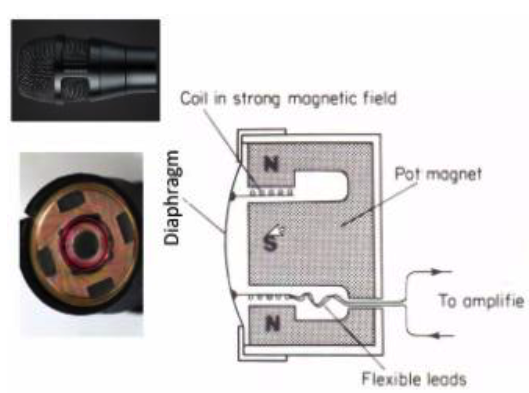
\includegraphics[height=0.2\textheight]{loudspeaker_cutaway.png}}
    \hfill
    \subfloat[Labeled cross-section]{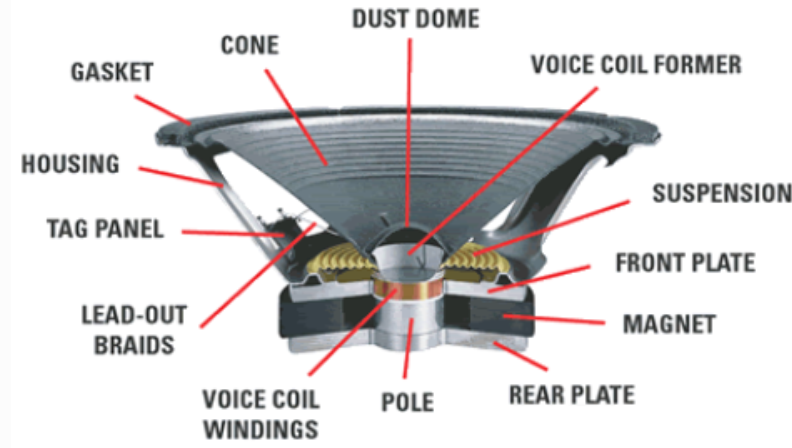
\includegraphics[height=0.2\textheight]{Loudspeaker_Structure.png}}
    \caption{An electrodynamic loudspeaker. The voice coil sits in the radial magnetic field formed between the pole piece and the front plate; the suspension and cone convert axial coil motion into acoustic radiation}
    \label{fig:loudspeakerStructure}
\end{figure}

\paragraph{Why the moving coil is called the voice coil} In the first generation of electrodynamic loudspeakers, permanent magnets powerful enough to produce a sufficiently intense gap field were not available. The static magnetic field was therefore generated by a second coil, wound directly on the magnetic circuit and energized by a DC supply, known as the field coil, because it produced the bias field rather than carrying the signal. The coil that carried the audio signal was distinguished from it by the name voice coil, signifying its role in reproducing the voice. With the advent of high-energy permanent-magnet materials (alnico in the 1930s, ferrite in the 1950s, neodymium in the 1980s), the field coil became obsolete; the name voice coil, however, was retained to designate the signal-carrying winding, and it remains in universal use in technical literature.

\subsection{The Lorentz Force on a Current-Carrying Conductor}

The fundamental law governing the electrodynamic transduction mechanism is the Lorentz force law. A point charge \(q\) moving with velocity \(\mathbf{u}\) in a magnetic field \(\mathbf{B}\) (measured in tesla, \(\si{\tesla} = \si{\newton\second\per\coulomb\per\meter}\)) experiences the vector force:
\[
\mathbf{F} = q \mathbf{u} \times \mathbf{B}
\]
The force is always perpendicular to both \(\mathbf{u}\) and \(\mathbf{B}\); its magnitude is:
\[
|\mathbf{F}| = q |\mathbf{u}| |\mathbf{B}| \sin\alpha
\]
where \(\alpha\) is the angle between the velocity of the charge and the field direction.

\begin{figure}[!htb]
    \centering
    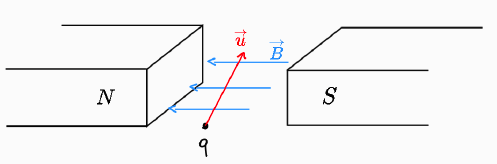
\includegraphics[width=0.50\linewidth]{lorentz_force.png}
    \caption{The Lorentz force on a positive charge \(q\) moving with velocity \(\mathbf{u}\) in a magnetic field \(\mathbf{B}\). The force \(\mathbf{F} = q \mathbf{u}\times\mathbf{B}\) is perpendicular to both vectors, with magnitude \(qu|\mathbf{B}|\sin\alpha\)}
\end{figure}

In a metallic conductor, many conduction electrons move simultaneously in response to an applied potential. For an infinitesimal volume element \(dV = S dl\) of a wire of cross-sectional area \(S\), the number of charge carriers is \(n dV\) (where \(n\) is the electron concentration per unit volume), and each contributes an infinitesimal Lorentz force:
\[
d\mathbf{F} = (-q \mathbf{u}\times\mathbf{B}) n dV
\]
Integrating over the full length \(L\) of the conductor:
\[
|\mathbf{F}| = n q |\mathbf{u}| |\mathbf{B}| \sin\alpha\cdot S L
\]
The electric current is the charge flowing per unit time: \(I = q n S |\mathbf{u}|\), so the expression simplifies to the compact motor law:

\begin{equation}
    |\mathbf{F}| = B l I \sin\alpha
    \label{eq:lorentzConductor}
\end{equation}

where \(l\) denotes the effective length of the wire in the field. In the loudspeaker, the voice coil is wound so that the current flow is perpendicular to the radial magnetic field at every point along the winding (\(\alpha = \pi/2\)), ensuring \(\sin\alpha = 1\) and, hence, the maximum possible force for a given current. Under this design condition, equation \eqref{eq:lorentzConductor} reduces to the fundamental motor law:
\[
F_C = B l i
\]

\begin{figure}[!htb]
    \centering
    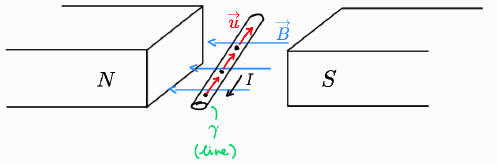
\includegraphics[width=0.50\linewidth]{wire_force.png}
    \caption{Infinitesimal wire element of cross-section \(S\) and length \(dl\) in a magnetic field \(\mathbf{B}\). Integrating the Lorentz force over the full winding length \(l\) yields the total axial force \(F_C = BlI\) when the current is perpendicular to the field}
\end{figure}

\subsection{Linearity and the Force Factor}

The product \(Bl\), called the force factor, with units \(\si{\newton\per\ampere} = \si{\tesla\meter}\), is the central electromagnetic parameter of the loudspeaker motor. The fundamental significance of the motor law \(F_C = Bl i\) lies in its linearity: if both \(B\) and \(l\) are constant throughout the voice coil's stroke, the driving force on the diaphragm is an exact linear replica of the driving current, with no additional harmonic or intermodulation content introduced at this stage of transduction. Conversely, any spatial variation of \(Bl\) with coil position, caused by inhomogeneities in the gap field, by flux modulation due to the signal current, or by the coil partially exiting the gap at large excursions, translates directly into harmonic and intermodulation distortion in the reproduced sound, degrading audio fidelity. The design of the magnetic circuit is therefore directed at maintaining the product \(Bl\) as spatially uniform as possible over the entire rated excursion of the voice coil.
The same Lorentz principle operates in the electrodynamic microphone, where the roles of force and motion are interchanged: acoustic pressure moves the diaphragm and the attached voice coil in the field, inducing a back-EMF proportional to the coil velocity, \(v = Bl u\), which constitutes the output electrical signal. The force factor \(Bl\) thus governs the transduction sensitivity in both directions, and maximizing it while maintaining spatial uniformity is common to both loudspeaker and microphone design.

\subsection{Electrical–Mechanical–Acoustical Conversion Chain}

The complete transduction path of a loudspeaker can be decomposed into three successive domain conversions, each governed by distinct physical laws:
\[
\text{Electrical}\;(v, i)
\;\longrightarrow\;
\text{Mechanical}\;(F, u)
\;\longrightarrow\;
\text{Acoustical}\;(P, U)
\]
At each interface the power variables of one domain are mapped to those of the next, while instantaneous power is conserved in the lossless idealization: electrical power \(P_E = v i\) becomes mechanical power \(P_M = F u\), which in turn becomes acoustic power \(P_A = P U\), where \(P\) is the acoustic pressure and \(U = u S_D\) is the volume velocity (the product of particle velocity and diaphragm area \(S_D\)). In practice, resistive losses in the voice coil (resistance \(R_{EC}\)), mechanical damping in the suspension (resistance \(R_{MS}\)), and the finite radiation resistance of the acoustic load all dissipate a fraction of the input power; a real loudspeaker typically converts less than \(2\%\) of the electrical input into radiated sound.

\begin{figure}[!htb]
    \centering
    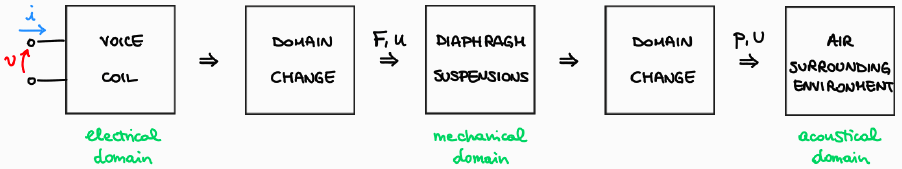
\includegraphics[width=0.75\textwidth]{conversion_chain.png}
    \caption{Block diagram of the loudspeaker transduction chain. Three physical domains are linked by two domain translations; each translation conserves instantaneous power (\(vi = Fu = PU\)) in the lossless idealization}
\end{figure}

The framework to be developed in the following chapter, the theory of electromechanical analogies, provides the mathematical tools for representing each domain and each domain translation as an equivalent electrical circuit element, so that the entire chain from electrical input to acoustic output can be analyzed with standard network-analysis methods.

\paragraph{Woofers and tweeters} The trade-off between moving mass, suspension compliance, and diaphragm area determines the usable frequency range of a driver. Woofers (low-frequency drivers) use large-area, relatively massive diaphragms to displace the air volume needed for efficient low-frequency radiation; tweeters (high-frequency drivers) use small, very light diaphragms so that the inertial reactance of the moving mass does not limit the response at high frequencies. These design constraints will be made quantitative once the full equivalent-circuit model of the loudspeaker is established in the chapters that follow.
    %! TEX root = main.tex

\graphicspath{{00_Images/02_chapter/}}

\chapter{Theory of Electromechanical Analogies}

The goal of the analogy theory is to represent mechanical and acoustical systems using the formalism of electrical circuit theory. This is not merely a notational convenience: because electrical circuit analysis offers a complete, systematic, and computationally powerful set of tools, Kirchhoff's laws, impedance combinations, Thévenin and Norton equivalents, frequency-domain methods, the ability to map a mechanical or acoustical system onto an equivalent electrical network allows all of these tools to be applied directly to the analysis of transducers, loudspeaker enclosures, and microphone capsules. The approach proceeds domain by domain: the electrical domain is reviewed first, the mechanical domain is introduced next by identifying its power variables and constitutive elements, and the two analogies that connect the two domains are then established and compared.

\section{The Electrical Domain}

The electrical domain is characterized by two power variables: voltage \(v\) (the potential difference between two nodes, measured in volts) and current \(i\) (the flow of charge through a branch, measured in amperes). The instantaneous electrical power delivered to a two-terminal element is \(P_E = v i\). Three ideal passive elements are used to model any linear, time-invariant (LTI) electrical network.

\paragraph{Resistor} A resistor of value \(R\) satisfies Ohm's law:
\[
v = R i
\]
It dissipates power (\(\bar P = R i_{\mathrm{RMS}}^2\)) and introduces no phase shift between voltage and current.

\paragraph{Capacitor} A capacitor of capacitance \(C\) (measured in farads, \(\si{\farad}\)) stores energy in its electric field. The constitutive relation is:
\[
i = C \frac{dv}{dt}
\qquad\Leftrightarrow\qquad
v(t) = \frac{1}{C}\int_0^t i(\tau) d\tau
\qquad\xrightarrow{\ \mathcal{L}\ }\qquad
V(s) = \frac{1}{sC} I(s)
\]
In steady sinusoidal operation the impedance is \(Z_C = 1/(j\omega C)\): the current leads the voltage by \(\pi/2\), and no net power is dissipated over one period.

\paragraph{Inductor} An inductor of inductance \(L\) (measured in henrys, \(\si{\henry}\)) stores energy in its magnetic field. The constitutive relation is:
\[
v = L \frac{di}{dt}
\qquad\Leftrightarrow\qquad
i(t) = \frac{1}{L}\int_0^t v(\tau) d\tau
\qquad\xrightarrow{\ \mathcal{L}\ }\qquad
I(s) = \frac{1}{sL} V(s)
\]
In sinusoidal operation the impedance is \(Z_L = j\omega L\): the voltage leads the current by \(\pi/2\), and no net power is dissipated.

\begin{figure}[!htb]
    \centering
    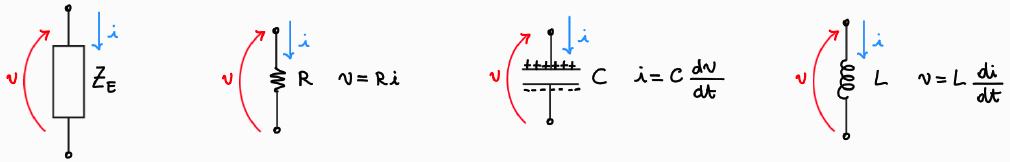
\includegraphics[width=0.85\textwidth]{electrical_elements.png}
    \caption{The three passive elements of the electrical domain: resistor (left), capacitor (center), and inductor (right), with their constitutive relations in the time domain}
\end{figure}

\paragraph{Alessandro Volta and the invention of the capacitor} A brief historical note is warranted here. Alessandro Volta (Como, 1745-1827), Professor of Physics at the University of Pavia from 1778, is universally known as the inventor of the electrochemical battery (the voltaic pile, demonstrated in 1799 and presented to Napoleon in Paris in 1801). Less commonly noted is that Volta had conceived and built the electrical condenser, the capacitor, even earlier, in 1789, as part of his work on electrometers for measuring electrostatic charge. Volta is therefore the inventor of not one but two of the three fundamental passive circuit elements, the capacitor and, indirectly through the battery, the voltage source. The unit of potential difference, the volt, commemorates his contributions, and the first international congress of physics held at Como in 1927, on the centenary of his death, brought together an extraordinary assembly of Nobel laureates including Lorentz, Planck, Bohr, Heisenberg, Fermi, and Pauli.

\section{The Mechanical Domain}

The mechanical domain is characterized by two power variables that play roles analogous to voltage and current in the electrical domain. The relevant variables for a one-dimensional mechanical system (such as the axial motion of a loudspeaker diaphragm) are force \(F\) (measured in newtons, \(\si{\newton}\)) and velocity \(u\) (measured in metres per second, \(\si{\meter\per\second}\)). The instantaneous mechanical power transmitted through a one-port mechanical element is:
\[
P_M = F u
\]
This is directly analogous to \(P_E = v i\) in the electrical domain, and it is this power equivalence that forms the physical basis for all electromechanical analogies. The displacement of the element is related to its velocity by \(x = \int u dt\). Three ideal mechanical elements, mass, spring (characterized by its compliance), and damper, describe the inertial, elastic, and dissipative behavior of any linear mechanical system.

\begin{figure}[!htb]
    \centering
    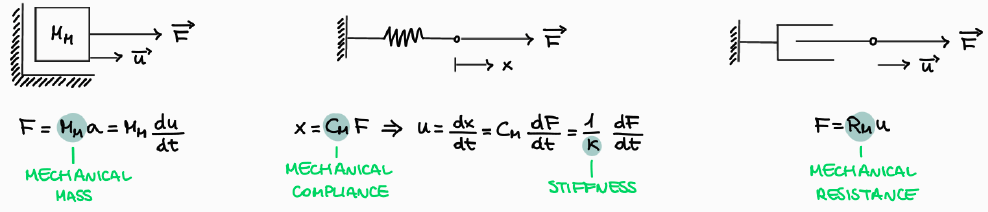
\includegraphics[width=0.80\textwidth]{mechanical_blocks.png}
    \caption{The three fundamental mechanical elements. Mass (left): \(F = M_M du/dt\). Spring with compliance \(C_M\) (center): \(u = C_M dF/dt\). Viscous damper (right): \(F = R_M u\). Each element is characterized by its constitutive relation between force and velocity}
\end{figure}

\subsection{Mechanical Mass}

The mechanical mass \(M_M\) (in kilograms, \(\si{\kilo\gram}\)) represents the inertia of a rigid body. By Newton's second law, the net force required to accelerate the mass is:
\[
F = M_M \frac{du}{dt}
\qquad\Leftrightarrow\qquad
u(t) = \frac{1}{M_M}\int_0^t F(\tau) d\tau
\]
In sinusoidal operation, with \(u = \tilde{u} e^{j\omega t}\), the force is \(F = j\omega M_M u\); the mechanical impedance of the mass is therefore \(Z_{M,\text{mass}} = j\omega M_M\), which increases linearly with frequency. The mass stores kinetic energy \(\frac{1}{2}M_M u^2\) but dissipates none; it is the mechanical analogue of the electrical inductor, because both elements oppose changes in the flow variable (current or velocity) by relating that variable to the time integral of the driving variable (voltage or force).

\subsection{Mechanical Compliance (Spring)}

The mechanical compliance \(C_M\) (in meters per newton, \(\si{\meter\per\newton}\)) is the reciprocal of the mechanical stiffness \(K = 1/C_M\). Hooke's law states that the displacement of a spring under a force \(F\) is proportional to the force:
\[
x = C_M F
\]
Differentiating both sides with respect to time gives the velocity-force constitutive relation:
\[
u = \frac{dx}{dt} = C_M \frac{dF}{dt}
\qquad\Leftrightarrow\qquad
F(t) = \frac{1}{C_M}\int_0^t u(\tau) d\tau
\]
In sinusoidal operation the mechanical impedance of the spring is \(Z_{M,\text{spring}} = 1/(j\omega C_M)\), which decreases with frequency and dominates the response at low frequencies. The spring stores potential energy \(\frac{1}{2}K x^2 = x^2/(2C_M)\) but dissipates none; it is the mechanical analogue of the electrical capacitor, because both elements relate the flow variable to the time integral of the driving variable (charge \(= \int i dt\) for the capacitor; displacement \(= \int u dt\) for the spring). The compliance \(C_M\) is thus the mechanical quantity that corresponds most naturally to electrical capacitance, and it is the parameter used to characterize the suspension of a loudspeaker or the diaphragm of a microphone.

\subsection{Mechanical Resistance (Damper)}
\label{ssc:523}

The mechanical damper (or dashpot) \(R_M\) (in newton-seconds per meter, \(\si{\newton\second\per\meter}\)) models viscous friction losses, the resistive force opposing velocity that arises from air friction, internal material damping in the suspension, or deliberate damping materials. Its constitutive relation is:
\[
F = R_M u
\qquad\Leftrightarrow\qquad
u = \frac{F}{R_M}
\]
The mechanical impedance of the damper is \(Z_{M,\text{damper}} = R_M\), independent of frequency. Power is dissipated as heat at the rate \(\bar P = R_M u_{\mathrm{RMS}}^2\). The damper is the mechanical analogue of the electrical resistor. Note that its reciprocal \(G_M = 1/R_M\) is the mechanical conductance (or mobility), measured in meters per newton-second; this quantity will arise naturally in the admittance analogy.

\paragraph{D'Alembert's principle for the diaphragm} In the loudspeaker, the voice coil exerts the driving force \(F_C = Bl i\) on the diaphragm, which is simultaneously subject to the spring restoring force of the suspension (\(F_S = x/C_{MS}\)), the viscous damping force (\(F_D = R_{MS} u\)), and its own inertial force (\(F_M = M_{MD} du/dt\)). D'Alembert's principle requires these forces to balance at every instant:
\[
F_C = F_S + F_D + F_M
= \frac{1}{C_{MS}}\int_0^t u(\tau) d\tau + R_{MS} u + M_{MD} \frac{du}{dt}
\]
This single equation, the mechanical equation of motion of the loudspeaker diaphragm, is the mechanical counterpart of Kirchhoff's voltage law for a series RLC circuit, a connection that the impedance analogy will make precise.

\section{Impedance and Admittance Analogies}

The objective of the analogy theory is to establish a one-to-one correspondence 
between the variables and elements of the mechanical domain and those of the 
electrical domain, so that an equivalent electrical circuit can be drawn for any 
mechanical system and analyzed by standard network methods. Two distinct analogies 
exist, each resting on a different identification of the mechanical power variables 
with the electrical ones. Both are physically valid; the choice between them is 
governed by considerations of topological clarity and computational convenience.

\subsection{Impedance Analogy (Type I)}

The variable mapping is:
\[
F \;\leftrightarrow\; v, \qquad u \;\leftrightarrow\; i
\]
so that the mechanical impedance \(Z_M = F/u\) maps directly onto the electrical 
impedance \(Z_E = v/i\).

\paragraph{Mechanical Mass}
\[
F = M_M \frac{du}{dt}
\;\xrightarrow{F\to v,\;u\to i}\;
v = M_M \frac{di}{dt} = L \frac{di}{dt}
\qquad\Longrightarrow\qquad
L = M_M
\]
The mechanical mass corresponds to an inductor.

\paragraph{Mechanical Compliance}
\[
u = C_M \frac{dF}{dt}
\;\xrightarrow{u\to i,\;F\to v}\;
i = C_M \frac{dv}{dt} = C \frac{dv}{dt}
\qquad\Longrightarrow\qquad
C = C_M
\]
The mechanical compliance corresponds to a capacitor.

\paragraph{Mechanical Resistance (Damper)}
\[
F = R_M u
\;\xrightarrow{F\to v,\;u\to i}\;
v = R_M i
\qquad\Longrightarrow\qquad
R = R_M
\]
The mechanical damper corresponds to a resistor.

\paragraph{Summary and topological rule}
\[
M_M \;\leftrightarrow\; L, \qquad C_M \;\leftrightarrow\; C, 
\qquad R_M \;\leftrightarrow\; R
\]
Since velocity maps to current, mechanical elements that share the same velocity 
experience the same current in the electrical circuit; they are therefore connected 
in series.

\subsection{Admittance Analogy (Type II)}

The variable mapping is:
\[
F \;\leftrightarrow\; i, \qquad u \;\leftrightarrow\; v
\]
so that the mechanical admittance \(Y_M = u/F\) maps directly onto the electrical 
admittance \(Y_E = i/v\).

\paragraph{Mechanical Mass}
\[
F = M_M \frac{du}{dt}
\;\xrightarrow{F\to i,\;u\to v}\;
i = M_M \frac{dv}{dt} = C \frac{dv}{dt}
\qquad\Longrightarrow\qquad
C = M_M
\]
The mechanical mass corresponds to a capacitor.

\paragraph{Mechanical Compliance}
\[
u = C_M \frac{dF}{dt}
\;\xrightarrow{u\to v,\;F\to i}\;
v = C_M \frac{di}{dt} = L \frac{di}{dt}
\qquad\Longrightarrow\qquad
L = C_M
\]
The mechanical compliance corresponds to an inductor.

\paragraph{Mechanical Resistance (Damper)}
\[
F = R_M u
\;\xrightarrow{F\to i,\;u\to v}\;
i = R_M v
\qquad\Longrightarrow\qquad
G_E = R_M, \quad R_E = \frac{1}{R_M}
\]
The mechanical damper corresponds to a conductance \(G_E = R_M\), represented 
in circuit diagrams as a resistor of value \(R_E = 1/R_M\).

\paragraph{Summary and topological rule}
\[
M_M \;\leftrightarrow\; C, \qquad C_M \;\leftrightarrow\; L, 
\qquad R_M \;\leftrightarrow\; G_E
\]
Since velocity maps to voltage, mechanical elements that share the same velocity 
experience the same voltage in the electrical circuit; they are therefore connected 
in parallel. This preserves the physical topology of the mechanical system: 
just as mass, compliance, and damper all connect the moving diaphragm to the fixed 
basket, the corresponding electrical elements all connect the same two nodes in the 
parallel circuit.

\begin{figure}[!htb]
    \centering
    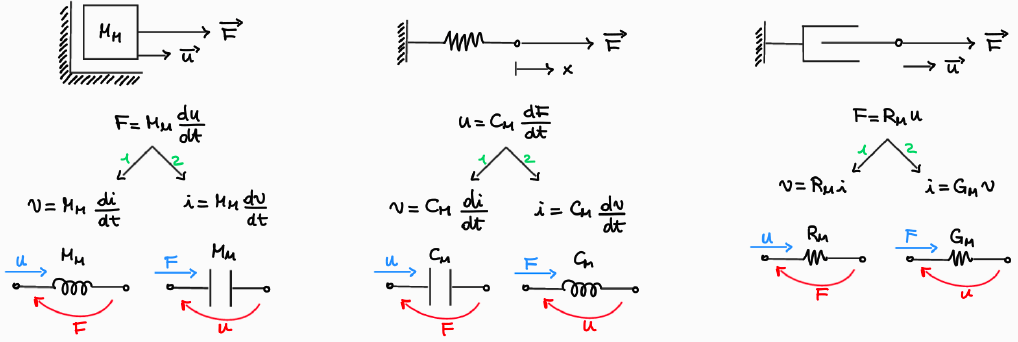
\includegraphics[width=0.85\textwidth]{impedance_admittance_analogies.png}
    \caption{Comparison of the impedance analogy (left) and the admittance analogy 
    (right) for the three fundamental mechanical elements. Under the impedance analogy, 
    common-velocity elements are in series; under the admittance analogy, they are in 
    parallel, preserving the visual topology of the mechanical system}
    \label{fig:analogiesComparison}
\end{figure}

\subsection{Summary of the Two Analogies}
\label{ssc:533}

Both analogies are mathematically equivalent: they produce identical predictions for all physical observables (impedance magnitude, frequency response, power, etc.) once the correct network topology is adopted. The choice is therefore one of convention and convenience. In loudspeaker analysis, where the diaphragm–suspension assembly has a natural parallel topology (all elements share the same velocity relative to the fixed basket), the admittance analogy is most common. In microphone and transmission-line analysis, where elements are naturally in series (they carry the same current or force in sequence), the impedance analogy may be preferred. The two choices will be kept explicit throughout this text, and the relevant analogy will be stated whenever a new equivalent circuit is introduced.

\begin{table}[!htb]
\centering
\renewcommand{\arraystretch}{1.3}
\begin{tabular}{|c|c|c|}
\hline
\textbf{Mechanical element} & \textbf{Impedance analogy} & \textbf{Admittance analogy} \\
& \textbf{Type I} & \textbf{Type II} \\
\hline
Force \(F\) & Voltage \(v\) & Current \(i\) \\
Velocity \(u\) & Current \(i\) & Voltage \(v\) \\
\hline
Mass \(M_M\) & Inductor \(L = M_M\) & Capacitor \(C = M_M\) \\
Compliance \(C_M\) & Capacitor \(C = C_M\) & Inductor \(L = C_M\) \\
Damper \(R_M\) & Resistor \(R = R_M\) & Conductance \(G = 1/R_M\) \\
\hline
Common-velocity elements & Series circuit & Parallel circuit \\
\hline
\end{tabular}
\caption{Variable mappings and element correspondences for the impedance analogy (Type I) and the admittance analogy (Type II). Both analogies are physically equivalent and produce the same predictions when the full network is analyzed}
\end{table}

\paragraph{Mechanical impedance and power} Regardless of which analogy is chosen, the mechanical impedance of a one-port element is defined as:
\[
Z_M = \frac{F}{u} = R_M + j X_M
\]
where \(R_M\) is the resistive (power-dissipating) part and \(X_M = \omega M_M - 1/(\omega C_M)\) is the reactive (energy-storing) part. The mean mechanical power delivered to the element is:
\[
\bar P_M = R_M u_{\mathrm{RMS}}^2
\]
confirming that only the resistive part of the mechanical impedance contributes to long-term energy dissipation, in complete analogy with the electrical case \(\bar P_E = \mathcal{R}\{Z_E\} I_{\mathrm{RMS}}^2\). This result will be used extensively in the analysis of loudspeaker efficiency and power handling in the chapters that follow.
    %%! TEX root = main.tex

\graphicspath{{00_Images/03_chapter/}}

\chapter{The Acoustic Domain}
\label{ch:acoustical_twoport}

The third domain in the transduction chain is the acoustical domain. Once the tools for mapping mechanical quantities to electrical ones are in place, extending the analogy to acoustics requires only identifying the correct power variables and deriving the constitutive relations for the three fundamental acoustic elements: mass, resistance, and compliance.

\section{Acoustic Variables and Fundamental Elements}
\label{sc:31}

In the acoustical domain the two power variables are acoustic pressure \(P\) (in pascal, \(\si{\pascal} = \si{\newton\per\meter\squared}\)) and volume velocity \(U\) (in cubic meters per second, \(\si{\cubic\meter\per\second}\)). Volume velocity is defined as:
\[
U = u \cdot S_D
\]
where \(u\) is the particle velocity and \(S_D\) is the cross-sectional area through which sound propagates, for instance the diaphragm area. The instantaneous acoustic power flowing through a cross-section is:
\[
P_A = P \cdot U
\]
This is the direct acoustic counterpart of \(P_E = v i\) in the electrical domain and of \(P_M = F u\) in the mechanical domain. The acoustic impedance of a one-port element is defined as:
\[
Z_A = \frac{P}{U} \quad \left[\frac{\si{\pascal}}{\si{\cubic\meter\per\second}} = \frac{\si{\newton\second}}{\si{\meter\tothe{5}}}\right]
\]
The specific acoustic impedance, which refers to particle velocity rather than volume velocity, is related to \(Z_A\) by \(Z_s = Z_A \cdot S\) and is measured in Rayls (\(\si{\pascal\second\per\meter}\)). For a plane wave in free air, the specific acoustic impedance equals the characteristic impedance of the medium, \(Z_0 = \rho_0 c \approx \SI{407}{\text{Rayl}}\).

\subsection{Acoustic Mass}
\label{ssc:311}

The acoustic mass \(M_A\) (in \(\si{\kilo\gram\per\meter\tothe{4}}\)) models the inertia of an air volume set in motion. It arises whenever a column of air is accelerated, for example inside a tube, a port, or the neck of a Helmholtz resonator. Its relation to the mechanical mass is:
\[
M_A = \frac{M_M}{S^2}
\]
because dividing the mechanical equation \(F = M_M du/dt\) by \(S^2\) and using \(P = F/S\), \(U = u S\) gives the acoustic constitutive relation:
\[
P = M_A \frac{dU}{dt}
\]
This has the same form as \(v = L di/dt\) for an inductor, so under the impedance analogy (\(P \leftrightarrow v\), \(U \leftrightarrow i\)), the acoustic mass corresponds to an inductor of value \(L_E = M_A\). Its acoustic impedance in the sinusoidal regime is \(Z_{M_A} = j\omega M_A\), which increases linearly with frequency and dominates the acoustic response at high frequencies.
Under the admittance analogy (\(P \leftrightarrow i\), \(U \leftrightarrow v\)), the same equation \(P = M_A dU/dt\) maps to \(i = C_E dv/dt\), so the acoustic mass corresponds to a capacitor of value \(C_E = M_A\). In practical terms, a large enclosed air volume behind a loudspeaker diaphragm contributes an acoustic mass load that appears, in the equivalent circuit, as either an inductor or a capacitor depending on the chosen analogy.

\begin{figure}[!htb]
    \centering
    \subfloat[Modeled as an inductor under the impedance analogy (\(P \leftrightarrow v\), \(U \leftrightarrow i\))]{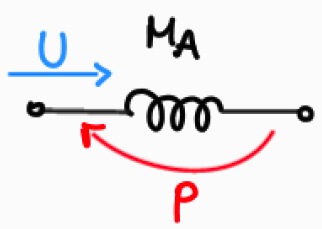
\includegraphics[width=0.3\linewidth]{acoustic_mass_impedance.png}}
    \hspace{1cm}
    \subfloat[Modeled as a capacitor under the admittance analogy (\(P \leftrightarrow i\), \(U \leftrightarrow v\))]{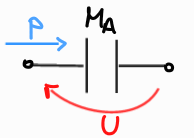
\includegraphics[width=0.3\linewidth]{acoustic_mass_admittance.png}}
    \caption{Both model of the acoustic mass}
\end{figure}

\subsection{Acoustic Resistance}
\label{ssc:312}

The acoustic resistance \(R_A\) (in \( \si{\newton\second\per\meter\tothe{5}} \)) models the power dissipated by viscous friction as air flows through a constriction such as a porous material, a narrow tube, or the perforations of a diaphragm. Starting from the mechanical damper relation \(F = R_M u\) and dividing by \(S^2\):
\[
P = R_A U, \qquad R_A = \frac{R_M}{S^2}
\]
This maps directly to \(v = R i\) in the electrical domain: under both the impedance and admittance analogies, the acoustic resistance corresponds to a resistor (or conductance, depending on the convention). Its acoustic impedance is purely real, \(Z_{R_A} = R_A\), independent of frequency, and mean power is dissipated at the rate \(\overline{P_A} = R_A U_\mathrm{RMS}^2\).
A practical acoustic resistance arises, for example, in a rectangular block of height \(2b\), width \(w\), and depth \(t\), drilled with cylindrical holes of radius \(a\). Each hole presents both a resistive and a mass contribution, with the resistance arising from viscosity and the mass from the inertia of the air slug inside the hole. Under the impedance analogy these two contributions appear in series, giving for each hole:
\[
Z_A = R_A + j\omega M_A
\]
with analytical expressions:
\[
R_A = \frac{1}{\pi a^2}\sqrt{\frac{2\omega\mu}{\rho_0}} \cdot \left[\frac{t}{a} + 2\left(1 - \frac{\pi a^2}{b^2}\right)\right],
\qquad
M_A = \frac{\rho_0}{\pi a^2}\left[t + 17a\left(1 - \frac{a}{b}\right)\right]
\]
where \(\mu\) is the dynamic viscosity of air and \(\rho_0\) is the air density. Such structures appear in loudspeaker cabinet design, microphone grilles, and acoustic absorption panels.

\subsection{Acoustic Compliance}
\label{ssc:313}

The acoustic compliance \(C_A\) (in \(\si{\meter\tothe{5}\per\newton}\)) models the elastic behavior of an enclosed volume of air. When a piston of area \(S\) compresses a cavity of volume \(V_0\), the restoring pressure is proportional to the fractional volume change, exactly as a spring restores a displaced mass. Starting from Hooke's law \(x = C_M F\) and converting to acoustic variables:
\[
U = C_A \frac{dP}{dt}, \qquad C_A = C_M S^2
\]
This has the same form as \(i = C dv/dt\) for a capacitor. Under the impedance analogy (\(P \leftrightarrow v\), \(U \leftrightarrow i\)), the acoustic compliance therefore corresponds to a capacitor of value \(C_E = C_A\). Its acoustic impedance is \(Z_{C_A} = 1/(j\omega C_A)\), which dominates the response at low frequencies. Under the admittance analogy (\(P \leftrightarrow i\), \(U \leftrightarrow v\)), differentiating the relation gives \(P = (1/C_A)\int U dt\), which maps to \(v = L di/dt\) for an inductor, so the acoustic compliance corresponds to an inductor.

\begin{figure}[!htb]
    \centering
    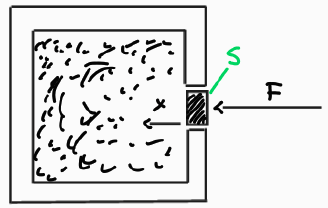
\includegraphics[width=0.5\linewidth]{acoustic_compliance_box.png}
    \caption{Acoustic compliance: a sealed box of volume \(V_0\) behind the diaphragm behaves as a spring. The equivalent acoustic compliance is \(C_A = V_0/(\rho_0 c^2)\) for an adiabatic process}
\end{figure}

For an adiabatic compression of an ideal gas in a rigid enclosure of volume \(V_0\), the acoustic compliance is:
\[
C_A = \frac{V_0}{\gamma P_0}
\]
where \(\gamma \approx 1.4\) is the ratio of specific heats and \(P_0 \approx \SI{101325}{\pascal}\) is the ambient pressure. A larger box is more compliant (softer spring), so its resonance with an acoustic mass occurs at a lower frequency. This is the physical basis for the dependence of a loudspeaker's bass response on enclosure volume.

\paragraph{Summary of acoustic element analogies} Under the impedance analogy, the acoustic mass maps to an inductor, the acoustic compliance maps to a capacitor, and the acoustic resistance maps to a resistor, with \(Z_A = P/U\) playing the role of electrical impedance. Under the admittance analogy, mass and compliance exchange their circuit roles (capacitor and inductor respectively), while resistance maps to a conductance. In both cases, acoustic power is conserved in the lossless elements and dissipated only in the acoustic resistance.

    %! TEX root = main.tex

\graphicspath{{00_Images/03_chapter/}}

\chapter{The Acoustic Domain}
\label{ch:acoustical_twoport}

The third domain in the transduction chain is the acoustical domain. Once the tools for mapping mechanical quantities to electrical ones are in place, extending the analogy to acoustics requires only identifying the correct power variables and deriving the constitutive relations for the three fundamental acoustic elements: mass, resistance, and compliance.

\section{Acoustic Variables and Fundamental Elements}
\label{sc:31}

The acoustical domain is characterized by two power variables. The acoustic pressure \(P\) (in pascal, \(\si{\pascal} = \si{\newton\per\meter\squared}\)) plays the role of the across-variable, analogous to voltage in the electrical domain or force in the mechanical domain. The volume velocity \(U\) (in \(\si{\cubic\meter\per\second}\)) plays the role of the through-variable, defined as:
\[
U = u \cdot S_D
\]
where \(u\) is the particle velocity and \(S_D\) is the cross-sectional area through which sound propagates. The instantaneous acoustic power flowing through a cross-section is:
\[
P_A = P \cdot U
\]
This is the direct acoustic counterpart of \(P_E = vi\) in the electrical domain and of \(P_M = Fu\) in the mechanical domain. The acoustic impedance of a one-port element is defined as:
\[
Z_A = \frac{P}{U}
\quad\left[\frac{\si{\pascal}}{\si{\cubic\meter\per\second}}
= \frac{\si{\newton\second}}{\si{\meter\tothe{5}}}\right]
\]
The specific acoustic impedance, which refers to particle velocity rather than volume velocity, is related to \(Z_A\) by \(Z_s = Z_A \cdot S\) and is measured in Rayls (\(\si{\pascal\second\per\meter}\)). For a plane wave in free air, the specific acoustic impedance equals the characteristic impedance of the medium, \(Z_0 = \rho_0 c \approx \SI{407}{\text{Rayl}}\).

\subsection{Acoustic Mass}
\label{ssc:311}

The acoustic mass \(M_A\) (in \(\si{\kilo\gram\per\meter\tothe{4}}\)) models the inertia of an air volume set in motion. It arises whenever a column of air is accelerated, for example inside a tube, a duct port, or the neck of a Helmholtz resonator. Starting from the mechanical equation \(F = M_M du/dt\) and substituting \(P = F/S\), \(U = uS\):
\[
M_A = \frac{M_M}{S^2}
\]
The acoustic constitutive relation is:
\[
P = M_A \frac{dU}{dt}
\qquad\Leftrightarrow\qquad
U(t) = \frac{1}{M_A}\int_0^t P(\tau) d\tau
\]
In sinusoidal operation the acoustic impedance of the mass is \(Z_{M_A} = j\omega M_A\), which increases linearly with frequency and dominates the acoustic response at high frequencies. The acoustic mass stores kinetic energy in the moving air slug but dissipates none.

\subsection{Acoustic Resistance}
\label{ssc:312}

The acoustic resistance \(R_A\) (in \(\si{\newton\second\per\meter\tothe{5}}\)) models the power dissipated by viscous friction as air flows through a constriction such as a porous material, a narrow tube, or the perforations of a diaphragm. Starting from the mechanical relation \(F = R_M u\) and substituting \(P = F/S\), \(U = uS\):
\[
R_A = \frac{R_M}{S^2}
\]
The acoustic constitutive relation is:
\[
P = R_A U
\qquad\Leftrightarrow\qquad
U = \frac{P}{R_A}
\]
Its acoustic impedance is purely real, \(Z_{R_A} = R_A\), independent of frequency, and mean acoustic power is dissipated at the rate \(\overline{P_A} = R_A U_{\mathrm{RMS}}^2\).

\paragraph{Practical example: perforated plate}
A rectangular block of height \(2b\), width \(w\), and depth \(t\), drilled with cylindrical holes of radius \(a\), presents both a resistive and a mass
contribution per hole. Under the impedance analogy these appear in series: \[
Z_A = R_A + j\omega M_A
\]
with analytical expressions:
\[
R_A = \frac{1}{\pi a^2}\sqrt{\frac{2\omega\mu}{\rho_0}}
\cdot\left[\frac{t}{a} + 2\!\left(1 - \frac{\pi a^2}{b^2}\right)\right],
\qquad
M_A = \frac{\rho_0}{\pi a^2}\left[t + 17a\!\left(1 - \frac{a}{b}\right)\right]
\]
where \(\mu\) is the dynamic viscosity of air. Such structures appear in loudspeaker cabinet design, microphone grilles, and acoustic absorption panels.

\subsection{Acoustic Compliance}
\label{ssc:313}

The acoustic compliance \(C_A\) (in \(\si{\meter\tothe{5}\per\newton}\)) models the elastic behavior of an enclosed volume of air. When a piston of area \(S\) compresses a cavity of volume \(V_0\), the restoring pressure is proportional to the fractional volume change, exactly as a mechanical spring restores a displaced mass. Starting from Hooke's law \(x = C_M F\), differentiating, and substituting \(U = uS\), \(P = F/S\):
\[
C_A = C_M S^2
\]
The acoustic constitutive relation is:
\[
U = C_A \frac{dP}{dt}
\qquad\Leftrightarrow\qquad
P(t) = \frac{1}{C_A}\int_0^t U(\tau) d\tau
\]
Its acoustic impedance is \(Z_{C_A} = 1/(j\omega C_A)\), which dominates the response at low frequencies. The acoustic compliance stores potential energy in the compressed air but dissipates none.

\begin{figure}[!htb]
    \centering
    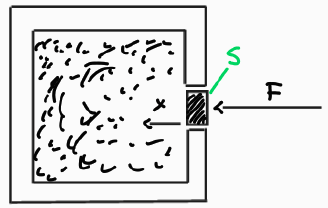
\includegraphics[width=0.5\linewidth]{acoustic_compliance_box.png}
    \caption{Acoustic compliance: a sealed box of volume \(V_0\) behind the
    diaphragm behaves as a spring. The equivalent acoustic compliance is
    \(C_A = V_0/(\rho_0 c^2)\) for an adiabatic process}
\end{figure}

For an adiabatic compression of an ideal gas in a rigid enclosure of volume \(V_0\), the acoustic compliance is:
\[
C_A = \frac{V_0}{\gamma P_0} = \frac{V_0}{\rho_0 c^2}
\]
where \(\gamma \approx 1.4\) is the ratio of specific heats, \(P_0 \approx \SI{101325}{\pascal}\) is the ambient pressure, and the equality \(\gamma P_0 = \rho_0 c^2\) holds for an adiabatic ideal gas. A larger box is more compliant, so its resonance with an acoustic mass occurs at a lower frequency, the physical basis for the dependence of a loudspeaker's bass response on enclosure volume.

\section{Acoustic Analogies}
\label{sc:32}

With the three acoustic elements defined, their mapping onto electrical circuit elements follows the same two analogies established in the mechanical domain. The acoustic power variables \((P, U)\) replace the mechanical pair \((F, u)\), and the acoustic impedance \(Z_A = P/U\) plays the same role as the mechanical impedance \(Z_M = F/u\).

\subsection{Impedance Analogy (Type I)}
\label{ssc:321}

The variable mapping is:
\[
P \;\leftrightarrow\; v, \qquad U \;\leftrightarrow\; i
\]
so that the acoustic impedance \(Z_A = P/U\) maps directly onto the electrical impedance \(Z_E = v/i\).

\paragraph{Acoustic Mass}
\[
P = M_A\frac{dU}{dt}
\;\xrightarrow{P\to v,\;U\to i}\;
v = M_A\frac{di}{dt} = L\frac{di}{dt}
\qquad\Longrightarrow\qquad
L_E = M_A
\]
The acoustic mass corresponds to an inductor.

\paragraph{Acoustic Resistance}
\[
P = R_A U
\;\xrightarrow{P\to v,\;U\to i}\;
v = R_A i
\qquad\Longrightarrow\qquad
R_E = R_A
\]
The acoustic resistance corresponds to a resistor.

\paragraph{Acoustic Compliance}
\[
U = C_A\frac{dP}{dt}
\;\xrightarrow{U\to i,\;P\to v}\;
i = C_A\frac{dv}{dt} = C\frac{dv}{dt}
\qquad\Longrightarrow\qquad
C_E = C_A
\]
The acoustic compliance corresponds to a capacitor.

\paragraph{Summary and topological rule}
\[
M_A \;\leftrightarrow\; L_E,
\qquad C_A \;\leftrightarrow\; C_E,
\qquad R_A \;\leftrightarrow\; R_E
\]
Since volume velocity maps to current, acoustic elements sharing the same volume velocity are connected in series in the equivalent circuit.

\subsection{Admittance Analogy (Type II)}
\label{ssc:322}

The variable mapping is:
\[
P \;\leftrightarrow\; i, \qquad U \;\leftrightarrow\; v
\]
so that the acoustic admittance \(Y_A = U/P\) maps directly onto the electrical admittance \(Y_E = i/v\).

\paragraph{Acoustic Mass}
\[
P = M_A\frac{dU}{dt}
\;\xrightarrow{P\to i,\;U\to v}\;
i = M_A\frac{dv}{dt} = C\frac{dv}{dt}
\qquad\Longrightarrow\qquad
C_E = M_A
\]
The acoustic mass corresponds to a capacitor.

\paragraph{Acoustic Resistance}
\[
P = R_A U
\;\xrightarrow{P\to i,\;U\to v}\;
i = R_A v
\qquad\Longrightarrow\qquad
G_E = R_A, \quad R_E = \frac{1}{R_A}
\]
The acoustic resistance corresponds to a conductance \(G_E = R_A\), represented in circuit diagrams as a resistor of value \(R_E = 1/R_A\).

\paragraph{Acoustic Compliance}
\[
U = C_A\frac{dP}{dt}
\;\xrightarrow{U\to v,\;P\to i}\;
v = C_A\frac{di}{dt} = L\frac{di}{dt}
\qquad\Longrightarrow\qquad
L_E = C_A
\]
The acoustic compliance corresponds to an inductor.

\paragraph{Summary and topological rule}
\[
M_A \;\leftrightarrow\; C_E,
\qquad C_A \;\leftrightarrow\; L_E,
\qquad R_A \;\leftrightarrow\; G_E
\]
Since volume velocity maps to voltage, acoustic elements sharing the same volume velocity are connected in parallel in the equivalent circuit.

\subsection{Summary of the Two Analogies}
\label{ssc:323}

Both analogies are mathematically equivalent and produce identical predictions for all physical observables once the correct network topology is adopted. The choice is governed by the natural topology of the system under analysis.

\begin{table}[!htb]
\centering
\renewcommand{\arraystretch}{1.3}
\begin{tabular}{|c|c|c|}
\hline
\textbf{Acoustic element} & \textbf{Impedance analogy} & \textbf{Admittance analogy} \\
                          & T\textbf{ype I}            & \textbf{Type II} \\
\hline
Pressure \(P\)       & Voltage \(v\) & Current \(i\) \\
Volume velocity \(U\) & Current \(i\) & Voltage \(v\) \\
\hline
Mass \(M_A\)        & Inductor \(L_E = M_A\)          & Capacitor \(C_E = M_A\) \\
Compliance \(C_A\)  & Capacitor \(C_E = C_A\)          & Inductor \(L_E = C_A\)  \\
Resistance \(R_A\)  & Resistor \(R_E = R_A\)           & Conductance \(G_E = R_A\) \\
\hline
Common-\(U\) elements & Series circuit & Parallel circuit \\
\hline
\end{tabular}
\caption{Variable mappings and element correspondences for the impedance analogy
(Type I) and the admittance analogy (Type II) in the acoustic domain. Both
analogies are physically equivalent; the choice is one of topological
convenience}
\label{tab:acousticAnalogies}
\end{table}

\paragraph{Acoustic impedance and power} Regardless of which analogy is chosen,
the acoustic impedance of a one-port element is:
\[
Z_A = \frac{P}{U} = R_A + jX_A
\]
where \(R_A\) is the resistive (power-dissipating) part and \(X_A = \omega M_A - 1/(\omega C_A)\) is the reactive (energy-storing) part. The mean acoustic power delivered to the element is:
\[
\overline{P_A} = R_A U_{\mathrm{RMS}}^2
\]
confirming that only the resistive part of the acoustic impedance contributes to net energy dissipation, in complete analogy with the electrical case \(\overline{P_E} = \mathcal{R}\{Z_E\} I_{\mathrm{RMS}}^2\) and the mechanical case \(\overline{P_M} = R_M u_{\mathrm{RMS}}^2\).

    %! TEX root = main.tex

\graphicspath{{00_Images/04_chapter/}}

\chapter{Complete Model of the Electrodynamic Loudspeaker}
\label{ch:loudspeaker_model}

With the three physical domains and their circuit analogues established and with the transformer and gyrator available as two-port elements for domain translation, it's possible to assemble the complete equivalent circuit model of the electrodynamic loudspeaker. The strategy is to work from the electrical terminals at one end to the acoustic radiation port at the other, inserting a two-port at each domain boundary. The result is a single electrical network that encodes the loudspeaker's behavior across all three domains, amenable to analysis with standard circuit tools. The chapter first introduces the two canonical two-port network elements that implement domain translations across the entire chain: the ideal transformer and the gyrator.

\section{Signal Transformers}

A signal transformer is a two-port network that converts a voltage-current pair \((v_p, i_p)\) at its primary port into a different voltage-current pair \((v_s, i_s)\) at its secondary port, while conserving instantaneous power. The fundamental relations of an ideal transformer with primary turns \(n_p\) and secondary turns \(n_s\), defining the turns ratio \(k = n_p/n_s\), are:
\begin{equation}
    \frac{v_p}{v_s} = \frac{n_p}{n_s} = k, \qquad \frac{i_s}{i_p} = k
    \label{eq:transformerRatio}
\end{equation}
Power conservation follows immediately: \(v_p i_p = (k v_s) (i_s/k) = v_s i_s\). The transformer is therefore a passive, lossless element: it redistributes voltage and current between ports but cannot amplify power.

\begin{figure}[!htb]
    \centering
    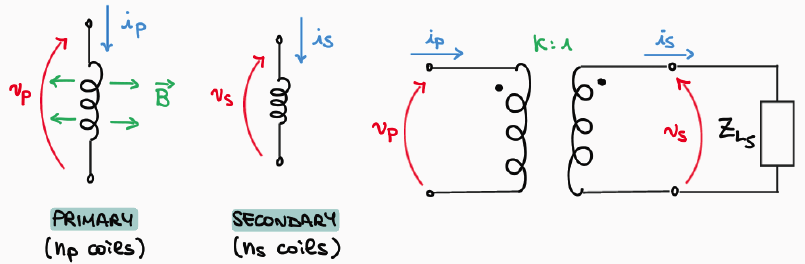
\includegraphics[width=0.65\linewidth]{signal_transformer.png}
    \caption{Ideal signal transformer with turns ratio \(k = n_p/n_s\). The voltage is scaled by \(k\) from primary to secondary; the current is scaled by \(1/k\). Power is conserved: \(v_p i_p = v_s i_s\)}
\end{figure}

\paragraph{Power grid example} A practical illustration of why the transformer is indispensable comes from electrical power transmission. Consider delivering \(P = \SI{1}{\mega\watt}\) of electrical power from a generating station to a city over a transmission line with resistance \(R_L\) per unit length. If the power is transmitted at low voltage (say \(v = \SI{10}{\kilo\volt}\)), the line current is \(i = P/v = \SI{100}{\ampere}\), and the resistive loss per kilometer is \(P_\mathrm{loss} = R_L i^2\), which at typical cable resistances amounts to roughly \SI{20}{\kilo\watt\per\kilo\meter}: a substantial fraction of the transmitted power. By inserting a step-up transformer at the generator to raise the voltage to \SI{380}{\kilo\volt}, the line current drops to \(i = P/v \approx \SI{2.6}{\ampere}\), and the resistive loss scales as \(i^2\), falling to approximately \SI{7}{\milli\watt\per\kilo\meter}: a reduction by a factor of nearly three million. A step-down transformer at the receiving end restores the voltage to a safe level for distribution. The transformer does not violate energy conservation; it simply trades current for voltage in a way that minimizes the dissipative penalty of line resistance.

\begin{figure}[!htb]
    \centering
    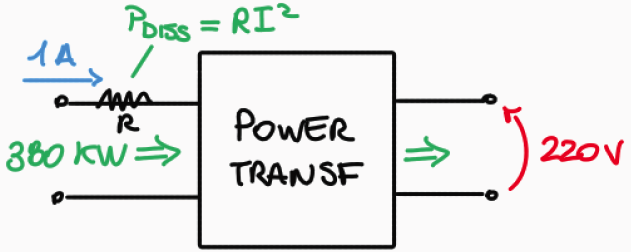
\includegraphics[width=0.8\textwidth]{power_transfer_block.png}
    \caption{High-voltage power transmission: a step-up transformer at the generator raises the voltage to \SI{380}{\kilo\volt} and reduces the current proportionally, cutting resistive line losses by the square of the voltage ratio. A step-down transformer restores usable voltage at the load}
\end{figure}

\subsection{Load Impedance Transformation}

A key property of the ideal transformer is that it modifies the impedance seen by the source. If the secondary port is loaded by an impedance \(Z_{LS} = v_s/i_s\), the impedance at the primary port is:
\[
Z_p = \frac{v_p}{i_p} = \frac{k v_s}{i_s/k} = k^2 \frac{v_s}{i_s}
\]
\begin{equation}
    Z_p = k^2 Z_{LS}
    \label{eq:impedanceTransform}
\end{equation}
A transformer with \(k > 1\) makes the load appear larger by a factor of \(k^2\) at the primary. This impedance scaling is exploited in audio engineering whenever the output impedance of a source must be matched to a load of different nominal impedance. A classic application is the output transformer of a vacuum-tube amplifier: the triode or pentode presents an output impedance of several kilohms, while a typical loudspeaker has a nominal impedance of \SI{4}{\ohm} to \SI{8}{\ohm}. The transformer scales the speaker impedance up so that it appears to the tube as the high-resistance load needed for efficient power transfer.
For example, a valve amplifier delivering \(P = \SI{100}{\watt}\) to a \SI{4}{\ohm} loudspeaker through a transformer with \(k = 20\) operates at primary voltage and current:
\[
i_p = \frac{i_s}{k} = \frac{5}{20} = \SI{250}{\milli\ampere}, \quad v_p = k v_s = 20 \times 20 = \SI{400}{\volt}
\]
The primary impedance is \(Z_p = k^2 Z_{LS} = 400 \times 4 = \SI{1600}{\ohm}\), a value compatible with the tube's operating point, while the secondary delivers the correct voltage and current to the speaker.

\begin{figure}[!htb]
    \centering
    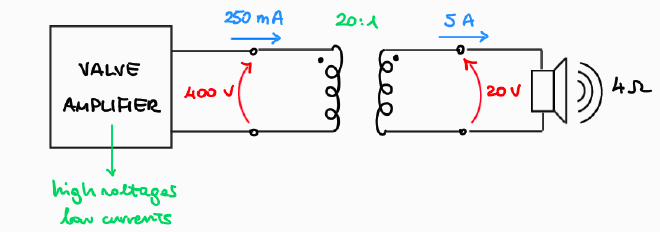
\includegraphics[width=0.6\linewidth]{valve_amp_to_loudspeaker.png}
    \caption{Impedance transformation in a valve amplifier: the output transformer scales the \SI{4}{\ohm} loudspeaker impedance up to \SI{1600}{\ohm} at the primary, matching the tube's operating conditions}
\end{figure}

\paragraph{Thevenin equivalent} When a Thevenin source with open-circuit voltage \(v_0\) and source impedance \(Z_0\) is connected to the primary, the equivalent Thevenin circuit seen from the secondary port has open-circuit voltage \(v_0/k\) and source impedance \(Z_0/k^2\). Both source voltage and source impedance are divided by \(k\) and \(k^2\) respectively when referred to the secondary side. This is a direct consequence of equation \eqref{eq:impedanceTransform} applied in reverse.

\begin{figure}[!htb]
    \centering
    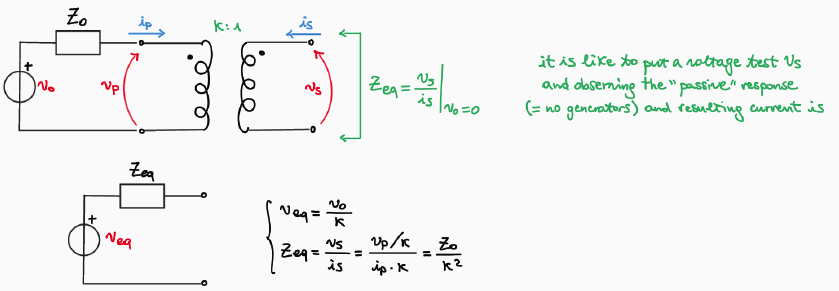
\includegraphics[width=0.75\linewidth]{Transformer_Thevenin_equiv.png}
    \caption{Thevenin equivalent of the signal transformer: a source \((v_0, Z_0)\) at the primary is seen from the secondary as a source \((v_0/k, Z_0/k^2)\)}
\end{figure}

\section{The Gyrator}
\label{sc:33}

The gyrator is a two-port network element introduced by Bernard Tellegen in 1948, the same researcher who formulated Tellegen's theorem in network theory and who is credited with conceiving the pentode vacuum tube. Tellegen proposed the gyrator as the fifth fundamental two-port, completing the canonical set of network elements alongside the resistor, capacitor, inductor, and transformer. Like the transformer, the gyrator is lossless: it transfers power from primary to secondary without dissipating energy. Unlike the transformer, it does not couple the two ports through a common magnetic flux but through a transconductance parameter \(g\) (in siemens, \(\si{\siemens} = \si{\ohm^{-1}}\)), which relates voltage on one port to current on the other in a crossed fashion.
The governing equations of the ideal gyrator are:
\begin{equation}
    i_s = g v_p, \qquad v_s = \frac{i_p}{g}
    \label{eq:gyratorLaws}
\end{equation}
from which it also follows that \(v_p = i_s/g\) and \(i_p = g v_s\). Power conservation is confirmed by:
\[
P_p = v_p i_p = \frac{i_s}{g}\cdot g v_s = v_s i_s = P_s
\]

\begin{figure}[!htb]
    \centering
    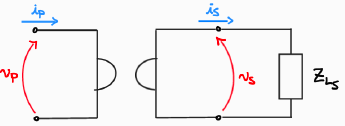
\includegraphics[width=0.45\linewidth]{gyrator_model.png}
    \caption{The ideal gyrator: transconductance \(g\) (in siemens) relates primary voltage to secondary current and vice versa. The element is lossless: \(v_p i_p = v_s i_s\)}
\end{figure}

\subsection{Impedance Inversion}
\label{ssc:331}

The most important property of the gyrator is impedance inversion. If the secondary port is loaded by an impedance \(Z_{LS} = v_s/i_s\), the primary input impedance is:
\[
Z_p = \frac{v_p}{i_p} = \frac{i_s/g}{g v_s} = \frac{1}{g^2}\cdot\frac{i_s}{v_s}
\]
\begin{equation}
    Z_p = \frac{1}{g^2 Z_{LS}} = \frac{Y_{LS}}{g^2}
    \label{eq:gyratorImpedance}
\end{equation}
The gyrator thus inverts the load impedance scaled by \(1/g^2\). This inversion exchanges the reactive nature of the secondary load as seen from the primary, with three notable consequences.

\paragraph{Resistive load} If \(Z_{LS} = R\), then \(Z_p = 1/(g^2 R) = G/g^2\) where \(G = 1/R\) is the load conductance. A resistor remains resistive at both ports, but its value is inverted.

\paragraph{Inductive load} If \(Z_{LS} = j\omega L\), then:
\[
Z_p = \frac{1}{g^2 j\omega L} = \frac{1}{j\omega C_\mathrm{eq}}, \qquad C_\mathrm{eq} = g^2 L
\]
An inductor at the secondary appears as a capacitor at the primary. This property is exploited in integrated-circuit design, where physical inductors are impractical: a gyrator loaded with a capacitor synthesizes a virtual inductor.

\paragraph{Capacitive load} If \(Z_{LS} = 1/(j\omega C)\), then:
\[
Z_p = \frac{j\omega C}{g^2} = j\omega L_\mathrm{eq}, \qquad L_\mathrm{eq} = \frac{C}{g^2}
\]
A capacitor at the secondary appears as an inductor at the primary. The gyrator therefore provides a complete duality between inductive and capacitive behavior.
The gyrator will reappear in Chapter 4 as the circuit representation of the electromechanical coupling in the impedance analogy: the motor law \(F = Bl i\) and the back-EMF law \(v = Bl u\) take precisely the form of equations \eqref{eq:gyratorLaws} with transconductance \(g = 1/(Bl)\).


\section{Domain Transductions}
\label{sc:41}

The loudspeaker pipeline connects three domains in sequence:
\[
\text{Electrical}\;(v, i)
\;\longrightarrow\;
\text{Mechanical}\;(F, u)
\;\longrightarrow\;
\text{Acoustical}\;(P, U)
\]
Each arrow represents a domain translation governed by the physical laws of the transduction mechanism. Both translations conserve instantaneous power in the lossless idealization.

\begin{figure}[!htb]
    \centering
    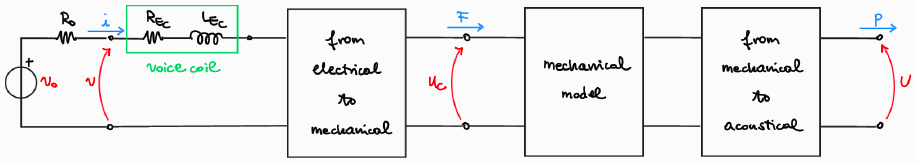
\includegraphics[width=0.90\textwidth]{loudspeaker_pipeline.png}
    \caption{The loudspeaker transduction chain: three physical domains linked by two domain translations. Each boundary is implemented as a two-port network element, either a transformer or a gyrator, depending on the analogy chosen}
\end{figure}

\subsection{Electrical to Mechanical Transduction}
\label{ssc:411}

The conversion from the electrical to the mechanical domain is governed by the Lorentz motor law. A current \(i\) flowing through a voice coil of effective length \(l\) in a magnetic field of flux density \(B\) generates the driving force:
\[
F_c = B l i
\]
Conversely, when the coil moves at velocity \(u_c\), a back-EMF is induced across the coil terminals according to Faraday's law:
\[
v = B l u_c \qquad \Longrightarrow \qquad u_c = \frac{v}{Bl}
\]
Written as a system, these two coupling equations are:
\[
\begin{cases}
    F_c = B l i \\[4pt]
    u_c = \dfrac{v}{B l}
\end{cases}
\]
Power is conserved across this translation: \(v i = (B l u_c) i = F_c u_c\), confirming that the electrical power input equals the mechanical power output in the lossless idealization.

\paragraph{Admittance analogy: transformer} Under the admittance analogy (\(F \leftrightarrow i\), \(u \leftrightarrow v\)), the coupling equations take the form:
\[
\frac{i}{F_c} = \frac{1}{Bl}, \qquad \frac{v}{u_c} = Bl
\]
This is exactly the transformer relation with turns ratio \(Bl\colon 1\). The primary port (electrical) carries current \(i\) and voltage \(v\); the secondary port (mechanical) carries force \(F_c \leftrightarrow i_s\) and velocity \(u_c \leftrightarrow v_s\).

\paragraph{Impedance analogy: gyrator} Under the impedance analogy (\(F \leftrightarrow v\), \(u \leftrightarrow i\)), the coupling equations become:
\[
i_s = g v_p \;\text{ with }\; g = \frac{1}{Bl}, \qquad v_s = \frac{i_p}{g}
\]
This matches the gyrator equations with transconductance \(g = 1/(Bl)\). The impedance analogy therefore represents the electromechanical coupling as a gyrator, and as a consequence of the impedance inversion property, the mechanical load impedance is inverted when referred to the primary electrical port.

\begin{figure}[!htb]
    \centering
    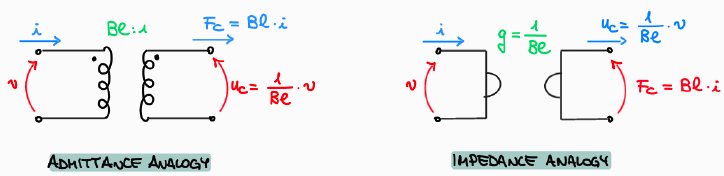
\includegraphics[width=0.70\linewidth]{imageE_M_analogies.png}
    \caption{Electrical-to-mechanical transduction under the admittance analogy (transformer with ratio \(Bl\colon 1\), left) and the impedance analogy (gyrator with \(g = 1/(Bl)\), right). The same physical law \(F = Bli\) is represented by two topologically different two-port elements}
\end{figure}

\subsection{Mechanical to Acoustical Transduction}
\label{ssc:412}

The conversion from the mechanical to the acoustical domain is governed by the geometry of the diaphragm. A diaphragm of area \(S_D\) translates mechanical force and velocity into acoustic pressure and volume velocity:
\[
\begin{cases}
    P = \dfrac{F}{S_D} \\[6pt]
    U = u S_D
\end{cases}
\]
Power is again conserved: \(P U = (F/S_D)(u S_D) = F u\). This translation has the form of a transformer with turns ratio \(1\colon S_D\) in both the admittance and impedance analogies.
%
%\begin{figure}[!htb]
%    \centering
%    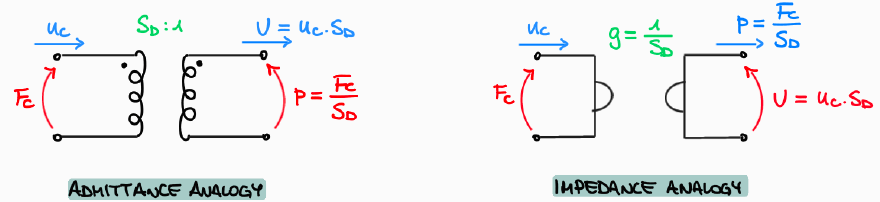
\includegraphics[width=0.80\linewidth]{M_A_Analogies.png}
%    \caption{Mechanical-to-acoustical transduction modeled as a transformer with ratio \(1\colon S_D\). The diaphragm area \(S_D\) sets the coupling in both analogies}
%\end{figure}

\section{Mechanical Section Modeling}
\label{sc:42}

The diaphragm and its suspension form the mechanical heart of the loudspeaker. The basket (frame) is mechanically rigid and is treated as the fixed reference, i.e., the ground node. The diaphragm of mass \(M_{MD}\) is connected to the basket through the suspension, which provides an elastic restoring force (modeled by the mechanical compliance \(C_{MS}\)) and viscous damping (modeled by the mechanical loss \(G_{MS}\)). The voice-coil velocity \(u_c\) equals the diaphragm velocity.
Three forces act on the diaphragm simultaneously: the spring restoring force \(F_S = x/C_{MS}\), where \(x = \int u dt\) is the displacement, giving \(u = C_{MS} dF_S/dt\); the damping force \(F_D = u / G_{MS}\); and the inertial force \(F_M = M_{MD} du/dt\). Applying d'Alembert's principle, the Lorentz driving force must balance the sum of all reaction forces at every instant:
\begin{equation}
    F_c = F_S + F_D + F_M = \frac{1}{C_{MS}}\int_0^t u(\tau) d\tau + R_{MS} u + M_{MD} \frac{du}{dt}
    \label{eq:dalembertDiaphragm}
\end{equation}

\paragraph{Admittance analogy: parallel RLC} Under the admittance analogy, velocity maps to voltage (\(u \leftrightarrow v\)) and force maps to current (\(F \leftrightarrow i\)). All three mechanical elements, the mass, the spring, and the damper, connect between the diaphragm node (at velocity \(u_c\)) and the basket node (at zero velocity). Because they all share the same velocity difference \(u_c\), they all have the same voltage in the equivalent circuit, which means they are connected in parallel. The driving force \(F_c\) is analogous to a current source, and by d'Alembert's equation \eqref{eq:dalembertDiaphragm} it is shared among the three parallel branches in direct analogy with Kirchhoff's current law at the diaphragm node. The mechanical section therefore maps to a parallel RLC circuit:
\[
M_{MD} \;\leftrightarrow\; C_{ED}, \qquad C_{MS} \;\leftrightarrow\; L_{ES}, \qquad G_{MS} \;\leftrightarrow\; R_{ES}
\]

\begin{figure}[!htb]
    \centering
    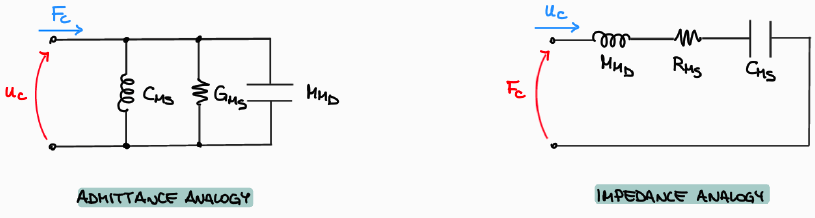
\includegraphics[width=0.85\textwidth]{mechanical_section_analogies.png}
    \caption{Mechanical section of the loudspeaker as a parallel RLC circuit (admittance analogy, left) and a series RLC circuit (impedance analogy, right). The admittance analogy is preferred because the parallel topology mirrors the actual physical arrangement: each element connects the moving diaphragm to the fixed basket}
\end{figure}

\paragraph{Impedance analogy: series RLC} Under the impedance analogy (\(F \leftrightarrow v\), \(u \leftrightarrow i\)), the common velocity \(u_c\) flows through all three elements in sequence, which is the analogue of Kirchhoff's voltage law for a series loop. The mechanical section maps to a series RLC circuit. The admittance analogy is nevertheless preferred for loudspeaker modeling, because the parallel topology visually preserves the physical arrangement of the mechanical system.

\section{The Full Equivalent Circuit and Impedance Reflection}
\label{sc:43}

Assembling all sub-models from the electrical input to the acoustic radiation port, the complete equivalent circuit of the loudspeaker in the admittance analogy consists of five cascaded stages:

\begin{enumerate}
    \item The voice coil is modeled as a series RL circuit with resistance \(R_{EC}\) (DC resistance of the winding) and inductance \(L_{EC}\) (inductance of the coil in the magnetic gap).
    \item The electrical-to-mechanical transduction is a transformer with turns ratio \(Bl\colon 1\).
    \item The mechanical section of the diaphragm-suspension assembly is a parallel RLC circuit.
    \item The mechanical-to-acoustical transduction is a transformer with turns ratio \(1\colon S_D\).
    \item The acoustic radiation environment is the radiation acoustic impedance \(Z_{AR} = \tilde{P}/\tilde{U}\).
\end{enumerate}

\begin{figure}[!htb]
    \centering
    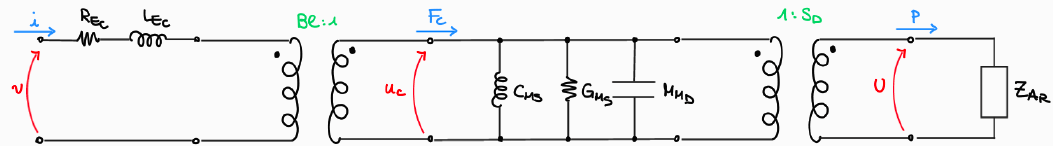
\includegraphics[width=0.95\textwidth]{loudspeaker_full_model.png}
    \caption{Complete equivalent circuit of the loudspeaker in the admittance analogy: voice-coil RL branch (\(R_{EC}\), \(L_{EC}\)), electromechanical transformer \(Bl\colon 1\), parallel RLC mechanical section (\(C_{MS}\), \(G_{MS}\), \(M_{MD}\)), mechano-acoustic transformer \(1\colon S_D\), and acoustic radiation admittance \(Y_{AR}\)}
    \label{fig:fullModel}
\end{figure}

\subsection{Referring All Elements to the Electrical Domain}
\label{ssc:431}

A practical strategy for circuit analysis is to reflect all elements through the transformers into a single domain, the electrical domain, eliminating both two-ports and obtaining a purely electrical network. The transformer relation \(v/i = (Bl)^2 u/F\) is used to convert each mechanical admittance to its electrical equivalent.

\paragraph{Diaphragm mass} Newton's second law gives \(F = M_{MD} du/dt\), so in the sinusoidal regime \(u/F = 1/(j\omega M_{MD})\). The electrical equivalent impedance is:
\[
\frac{v}{i} = (Bl)^2\cdot\frac{u}{F} = \frac{(Bl)^2}{j\omega M_{MD}} = \frac{1}{j\omega C_{ED}}, \qquad C_{ED} = \frac{M_{MD}}{(Bl)^2}
\]
The diaphragm mass corresponds to an equivalent electrical capacitance \(C_{ED}\). Since typical designs require \(C_{ED}\) of the order of nanofarads, a light diaphragm is desirable.

\begin{figure}[!htb]
    \centering
    \subfloat{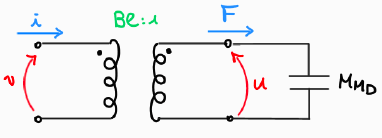
\includegraphics[height=0.15\textheight]{Diaphragm_capacitor_M_MD.png}}
    \hfill
    \subfloat{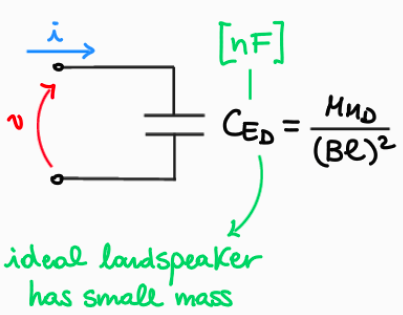
\includegraphics[height=0.15\textheight]{Diaphragm_capacitor_C_ED.png}}
    \caption{Diaphragm mass \(M_{MD}\) in the mechanical domain (left) and its electrical equivalent capacitance \(C_{ED} = M_{MD}/(Bl)^2\) (right). A lighter diaphragm produces a smaller \(C_{ED}\), which raises the resonance frequency}
\end{figure}

\paragraph{Suspension compliance} The compliance relation \(u = C_{MS} dF/dt\) gives \(u/F = j\omega C_{MS}\) in the sinusoidal regime. The electrical equivalent is:
\[
\frac{v}{i} = (Bl)^2\cdot j\omega C_{MS} = j\omega L_{ES}, \qquad L_{ES} = (Bl)^2 C_{MS}
\]
The suspension compliance corresponds to an equivalent electrical inductance \(L_{ES}\).

\begin{figure}[!htb]
    \centering
    \subfloat{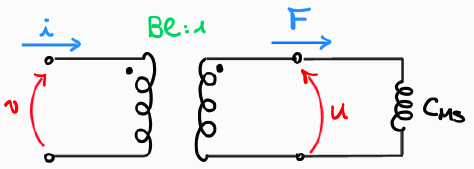
\includegraphics[height=0.12\textheight]{electrical_suspension_inductance.png}}
    \hfill
    \subfloat{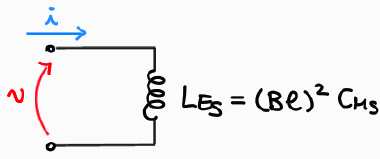
\includegraphics[height=0.12\textheight]{electrical_suspension_inductance_2.png}}
    \caption{Electrical equivalent of the suspension compliance: \(L_{ES} = (Bl)^2 C_{MS}\). A softer suspension (larger \(C_{MS}\)) produces a larger \(L_{ES}\) and lowers the resonance frequency}
\end{figure}

\paragraph{Suspension losses} The mechanical conductance \(G_{MS} = 1/R_{MS}\) gives \(u/F = G_{MS}\). The electrical equivalent is:
\[
\frac{v}{i} = (Bl)^2 G_{MS} \;\Longrightarrow\; R_{ES} = (Bl)^2G_{MS} = \frac{(Bl)^2}{R_{MS}}
\]
The suspension damping corresponds to an equivalent electrical resistance \(R_{ES}\). Note that a higher mechanical resistance (stronger damping) results in a lower \(R_{ES}\), because the bridge passes through a conductance.

\begin{figure}[!htb]
    \centering
    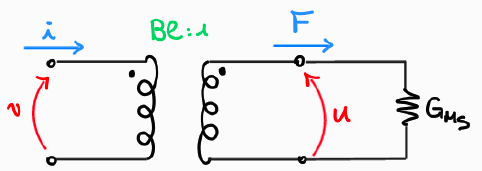
\includegraphics[width=0.70\linewidth]{electrical_suspension_resistance_0.png}
    \caption{Electrical equivalent of the suspension damping: \(R_{ES} = (Bl)^2/R_{MS}\). A more heavily damped suspension reduces \(R_{ES}\) and broadens the impedance resonance peak}
\end{figure}

\paragraph{Acoustic radiation impedance} The acoustic radiation admittance \(Y_{AR} = U/P\) is referred back to the electrical domain in two explicit steps.

\begin{enumerate}
    \item Acoustic to mechanical (transformer \(1\colon S_D\)): The mechano-acoustic coupling relations \(P = F/S_D\) and \(U = u\,S_D\) give directly:
    \[
    \frac{u}{F} = \frac{1}{S_D^2}\cdot\frac{U}{P}
    \qquad\Longrightarrow\qquad
    Y_{MR} = \frac{Y_{AR}}{S_D^2}
    \]
    Under the admittance analogy, \(Y_{MR} = u/F \leftrightarrow v/i = Z_{E}\), so the mechanical radiation admittance appears as an electrical impedance.
    \item Mechanical to electrical (transformer \(Bl\colon 1\)): The electromechanical coupling gives:
    \[
    \frac{v}{i} = (Bl)^2\cdot\frac{u}{F}
    \qquad\Longrightarrow\qquad
    Z_{ER} = (Bl)^2\,Y_{MR}
    \]
    Substituting the result of Step 1:
    \[
    Z_{ER} = (Bl)^2\cdot\frac{Y_{AR}}{S_D^2}
    = \left(\frac{Bl}{S_D}\right)^{2} Y_{AR}
    \]
\end{enumerate}

\subsection{The Overall Electrical Equivalent}
\label{ssc:432}

By combining all reflected elements, the complete loudspeaker reduces to a single electrical two-terminal network. The total electrical impedance decomposes as:
\[
Z_E = Z_{ES} + Z_{EM}
\]
where the series part collects the voice-coil elements:
\[
Z_{ES} = R_{EC} + j\omega L_{EC}
\]
and the parallel part groups the remaining reflected elements:
\[
Z_{EM} = Z_{L_{ES}}  ||  R_{ES}  ||  Z_{C_{ED}}  ||  Z_{ER}
\]

\begin{figure}[!htb]
    \centering
    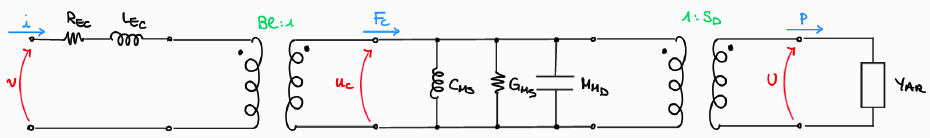
\includegraphics[width=0.90\textwidth]{overall_mechanical_model.png}
    \caption{Overall electrical equivalent circuit referred entirely to the electrical domain. Every mechanical and acoustical elements are represented by their electrical analogues}
\end{figure}

\begin{figure}[!htb]
    \centering
    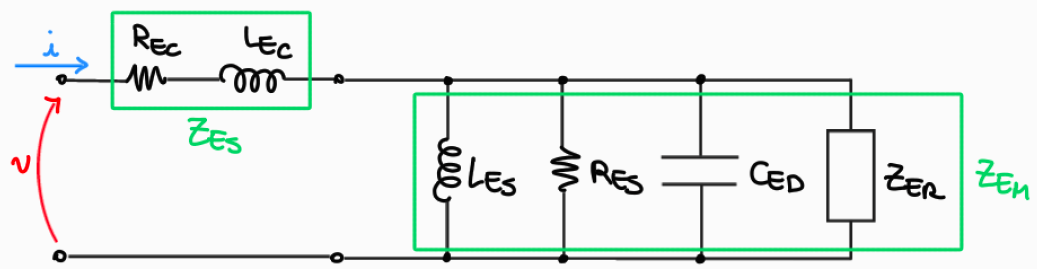
\includegraphics[width=0.70\textwidth]{overall_model_2.png}
    \caption{Simplified representation: the series block \(Z_{ES}\) and the parallel block \(Z_{EM}\) resonate at the fundamental frequency \(f_s\) of the diaphragm-suspension system}
\end{figure}

The parallel block \(Z_{EM}\) is a resonant RLC circuit. Its resonance frequency is:
\[
f_s = \frac{1}{2\pi\sqrt{L_{ES} C_{ED}}} = \frac{1}{2\pi\sqrt{(Bl)^2 C_{MS}\cdot M_{MD}/(Bl)^2}} = \frac{1}{2\pi\sqrt{M_{MD} C_{MS}}}
\]
which is precisely the fundamental mechanical resonance of the diaphragm-suspension system: the \(Bl\) factors cancel, confirming that \(f_s\) is a purely mechanical parameter independent of the magnetic circuit strength. At \(f = f_s\), the inductive and capacitive reactances in the parallel branch cancel and \(Z_{EM}\) reaches its maximum, which is the purely resistive value \(R_{ES}\). The total loudspeaker impedance therefore shows a pronounced peak at \(f_s\), the measurable feature used in practice to determine the Thiele-Small parameters of a driver.

\paragraph{Design implications of the model} The power of the equivalent-circuit approach lies in translating multi-physics design questions into familiar circuit terms. Doubling the diaphragm mass \(M_{MD}\) doubles \(C_{ED}\) and lowers \(f_s\) by \(\sqrt{2}\). Stiffening the suspension (reducing \(C_{MS}\)) reduces \(L_{ES}\) and raises \(f_s\). Weakening the magnetic gap (reducing \(Bl\)) lowers the transformer turns ratio, reducing coupling and increasing the effective mechanical load seen from the electrical terminals, thereby degrading efficiency. Increasing the diaphragm area \(S_D\) alters the acoustic transformer ratio and changes the reflected radiation impedance \(Z_{ER}\). All of these predictions follow from the circuit by inspection, without measurement or numerical simulation, which is the central advantage of the analogy-based modeling approach.

    %! TEX root = main.tex

\graphicspath{{00_Images/05_chapter/}}

\chapter{Power in Audio Signals}
\label{ch:power}

Electrical power, mechanical power, and acoustic power are all described by the same mathematical structure: the product of two conjugate variables, one a pressure-like quantity and the other a flow-like quantity. In the electrical domain this is voltage times current; in the mechanical domain, force times velocity; in the acoustic domain, pressure times volume velocity. The challenge specific to audio engineering is that none of these signals is constant in time: musical waveforms are complex, non-periodic, and span many orders of magnitude in amplitude within a single piece. This chapter establishes the tools needed to quantify power in such signals, with particular attention to the distinction between mean and peak power and to the consequences for amplifier and transducer design.

\section{Electrical Power, RMS, and Crest Factor}
\label{sc:51}

The instantaneous electrical power delivered to a two-terminal element is:
\[
W_E(t) = v(t) i(t)
\]
For a purely resistive load \(R\), this becomes \(W_E(t) = v^2(t)/R\). Because audio signals have zero mean value by construction, the instantaneous power has a non-zero time-average even though the signal itself averages to zero. The physically relevant quantity is the mean power, defined as the time-average of the instantaneous power over a representative interval \(T\):
\[
\overline{W} = \frac{1}{T}\int_0^T W_E(t) dt = \frac{1}{R}\cdot\frac{1}{T}\int_0^T v^2(t) dt = \frac{v_\mathrm{RMS}^2}{R}
\]
where the Root Mean Square (RMS) voltage is:
\[
v_\mathrm{RMS} = \sqrt{\frac{1}{T}\int_0^T v^2(t) dt}
\]
The RMS value is the equivalent constant voltage that would dissipate the same energy in the resistance as the time-varying signal \(v(t)\). For a sinusoid \(v(t) = V_P\sin(\omega t)\), direct integration gives \(v_\mathrm{RMS} = V_P/\sqrt{2}\), which corresponds to a level 3 dB below the peak. The mean and peak power on a resistive load are then:
\[
\overline{W} = \frac{V_P^2}{2R}, \qquad W_\mathrm{peak} = \frac{V_P^2}{R} = 2 \overline{W}
\]

\paragraph{Musical signals in practice} Real musical waveforms are far more complex than a single sinusoid. The RMS value and the peak value both vary continuously as a function of the musical content, and the ratio between them changes from one moment to the next. The three intervals shown in the figure below illustrate how the same song can have very different peak-to-RMS ratios depending on the density and transient content of the passage.

\begin{figure}[!htb]
    \centering
    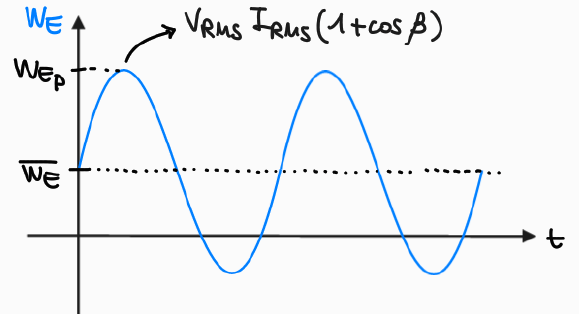
\includegraphics[width=0.85\textwidth]{electrical_power_wf.png}
    \caption{Three seconds of a typical musical signal divided into successive intervals. The RMS voltage (proportional to mean power) and the peak voltage vary independently across intervals, showing that both mean power and peak power are time-dependent quantities for audio signals}
\end{figure}

\subsection{The Crest Factor}
\label{ssc:511}

The ratio between peak power and mean power is called the Crest Factor (CF):
\begin{equation}
    CF = \frac{W_\mathrm{peak}}{\overline{W}}
    \label{eq:crestFactor}
\end{equation}
Expressed in decibels:
\[
CF_\mathrm{dB} = 10\log_{10}(CF)
\]
For a pure sinusoid, \(CF = 2\ (+\SI{3}{\decibel})\), because the peak power is exactly twice the mean power. For a complex musical signal, the crest factor is typically 4 or higher (\(\geq +6\) dB), and it depends on the time interval over which peak and mean values are measured: a transient-rich passage such as a percussion hit has a much higher crest factor than a sustained, compressed chord.
The crest factor has direct engineering implications. An amplifier must be capable of delivering the peak power without clipping, even if the mean power it supplies is much lower. If an amplifier is rated at a continuous output power \(\overline{W}\), and the musical signal has \(CF = 4\), then the amplifier must instantaneously supply \(4\overline{W}\) without distortion. Underestimating the crest factor leads to clipping on transients, which produces odd-order harmonic distortion and, more critically, can deliver sustained high-frequency content to a tweeter whose thermal rating is based on mean power: the voice coil overheats and the driver fails even though the rated mean power was never exceeded. Crest factor is therefore a key parameter for amplifier headroom specification and for loudspeaker thermal protection design.

\section{Power in a Generic Impedance}
\label{sc:52}

When the load is a complex impedance \(Z_E = R_E + jX_E\) rather than a pure resistance, voltage and current are no longer in phase, and the relationship between instantaneous and mean power requires a more careful treatment.
Consider a sinusoidal voltage \(v(t) = V\sin(\omega t)\) applied to an impedance \(Z_E\). The resulting current lags or leads the voltage by the phase angle \(\beta\):
\[
i(t) = I\sin(\omega t + \beta), \qquad I = \frac{V}{|Z_E|}
\]
The instantaneous power is:
\[
W_E(t) = v(t) i(t) = VI\sin(\omega t)\sin(\omega t + \beta)
\]
Expanding with the product-to-sum trigonometric identity:
\[
W_E(t) = \frac{VI}{2}\cos(\beta) - \frac{VI}{2}\cos(2\omega t + \beta)
\]
In RMS quantities (\(V_\mathrm{RMS} = V/\sqrt{2}\), \(I_\mathrm{RMS} = I/\sqrt{2}\)):
\[
W_E(t) = \underbrace{V_\mathrm{RMS} I_\mathrm{RMS}\cos(\beta)}_{\overline{W_E},\text{ constant}} - \underbrace{V_\mathrm{RMS} I_\mathrm{RMS}\cos(2\omega t + \beta)}_{\text{zero mean oscillation}}
\]
The time-average of the oscillating second term is zero over any complete cycle, so the mean power is:
\begin{equation}
    \overline{W_E} = V_\mathrm{RMS} I_\mathrm{RMS}\cos(\beta)
    \label{eq:meanPowerPhase}
\end{equation}

\subsection{In-Phase and Quadrature Decomposition}
\label{ssc:521}

The result of equation \eqref{eq:meanPowerPhase} can be made more transparent by decomposing the current into two components relative to the voltage. The in-phase component carries the portion of the current that is synchronized with the voltage:
\[
i_p(t) = I\cos\beta \sin(\omega t), \qquad i_q(t) = I\sin\beta \cos(\omega t)
\]
where \(i_p\) is exactly in phase with \(v(t)\) and \(i_q\) is 90 degrees out of phase (in quadrature). The instantaneous power separates accordingly:
\[
W_E(t) = v(t) i_p(t) + v(t) i_q(t) = W_{E,p}(t) + W_{E,q}(t)
\]
The active power component \(W_{E,p}(t) = V_\mathrm{RMS}I_{p,\mathrm{RMS}}[1 - \cos(2\omega t)]\) is always non-negative and has a positive mean equal to \(V_\mathrm{RMS}I_{p,\mathrm{RMS}}\): it represents energy flowing steadily from the source into the load, where it is converted into heat (in a resistance) or into mechanical or acoustic work. The reactive power component \(W_{E,q}(t) = V_\mathrm{RMS}I_{q,\mathrm{RMS}}\sin(2\omega t)\) oscillates symmetrically about zero and has a mean of exactly zero: it represents energy that is stored in the reactive element during one quarter-cycle and returned to the source during the next, with no net transfer per full cycle.
From the impedance relation \(i(t) = v(t)/Z_E\), one can extract the in-phase conductance:
\[
i_p(t) = \frac{\mathcal{R}\{Z_E\}}{|Z_E|^2} v(t)
\]
so the mean power is:
\[
\overline{W_E} = \frac{\mathcal{R}\{Z_E\}}{|Z_E|^2} V_\mathrm{RMS}^2
\]
Since \(I_\mathrm{RMS} = V_\mathrm{RMS}/|Z_E|\), this is equivalent to:
\begin{equation}
    \overline{W_E} = \mathcal{R}\{Z_E\} I_\mathrm{RMS}^2
    \label{eq:meanPowerZ}
\end{equation}
This result confirms that mean power is determined exclusively by the resistive (real) part of the impedance. The reactive part \(X_E\) shifts the phase between voltage and current, reduces the effective power factor \(\cos\beta\), and increases the current amplitude required to deliver a given mean power, but it contributes nothing to the time-averaged energy transfer.

\paragraph{Special cases} For a purely resistive load (\(X_E = 0\), \(\beta = 0\)): \(\overline{W_E} = V_\mathrm{RMS}^2/R_E\), the maximum possible power for a given voltage. For a purely reactive load (\(R_E = 0\), \(\beta = \pm\pi/2\)): \(\overline{W_E} = 0\), regardless of how large the instantaneous power swings become. A loudspeaker presents a complex impedance at almost all audio frequencies, so the power factor \(\cos\beta\) is always less than unity; this is why amplifiers must be rated for reactive loads and not merely for resistive ones.

\section{Mechanical and Acoustical Power}
\label{sc:53}

The same decomposition into active and reactive components applies in the mechanical and acoustic domains, with the appropriate substitution of power variable pairs.

\subsection{Mechanical Power}
\label{ssc:531}

The instantaneous mechanical power transmitted through a one-port mechanical element is \(W_M(t) = F(t) u(t)\). The mechanical impedance is defined as \(Z_M = F/u = R_M + jX_M\), where \(R_M\) is the mechanical resistance and \(X_M = \omega M_M - 1/(\omega C_M)\) is the reactive part. Under the admittance analogy, force maps to current and velocity maps to voltage, so the result of equation \eqref{eq:meanPowerZ} translates directly to:
\[
\overline{W_M} = R_M u_\mathrm{RMS}^2
\]
Only the resistive component of the mechanical impedance is responsible for net energy dissipation. In the loudspeaker, the total mechanical resistance has two contributions: the suspension damping \(R_{MS}\), which converts mechanical energy into heat within the spider and surround, and the mechanical radiation resistance \(R_{MR}\), which is the part of the mechanical load that transfers energy outward as acoustic radiation.

\begin{figure}[!htb]
    \centering
    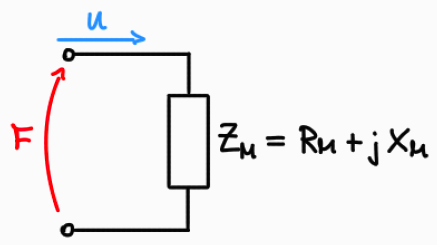
\includegraphics[width=0.35\textwidth]{mechanical_impedance_block.png}
    \caption{Mechanical one-port with impedance \(Z_M = R_M + jX_M\). The mean mechanical power is \(\overline{W}_M = R_M u_\mathrm{RMS}^2\); the reactive energy oscillates between mass and compliance without net loss}
\end{figure}

\subsection{Acoustical Power and the Radiation Resistance}
\label{ssc:532}

The instantaneous acoustic power is \(W_A(t) = P(t) U(t)\). The acoustic impedance is \(Z_A = P/U = R_A + jX_A\), and the mean radiated acoustic power is:
\[
\overline{W_A} = R_A U_\mathrm{RMS}^2 = \frac{\mathcal{R}\{Z_A\}}{|Z_A|^2} P_\mathrm{RMS}^2
\]

\begin{figure}[!htb]
    \centering
    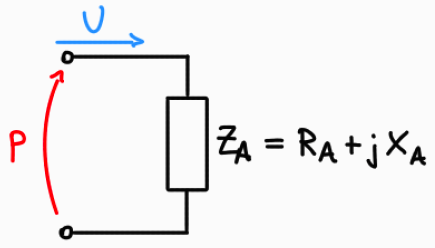
\includegraphics[width=0.40\textwidth]{acoustic_port_block.png}
    \caption{Acoustic one-port with impedance \(Z_A = R_A + jX_A\). Only \(R_A = \mathcal{R}\{Z_A\}\) contributes to net radiated acoustic power}
\end{figure}

For a loudspeaker, the acoustic radiation impedance at the diaphragm is \(Z_{AR} = R_{AR} + jX_{AR}\), where \(R_{AR}\) is the radiation resistance that converts diaphragm motion into propagating sound waves. Substituting the volume velocity \(U = u_c S_D\):
\[
\overline{W_A} = R_{AR} U_\mathrm{RMS}^2 = R_{AR} (u_c S_D)^2 = R_{MR} u_{c,\mathrm{RMS}}^2
\]
where the mechanical radiation resistance is:
\begin{equation}
    R_{MR} = S_D^2 R_{AR}
    \label{eq:mechanicalRadiation}
\end{equation}
Referred back through the electromechanical coupling \(F = Bl i_c\), and assuming that the coil inductance is negligible at the frequencies of interest (\(\omega L_{EC} \ll R_g + R_{EC}\)), the driving force is \(F_\mathrm{RMS} = Bl v_{g,\mathrm{RMS}}/(R_g + R_{EC})\), and the complete expression for radiated acoustic power as a function of generator voltage is:
\[
\overline{W_A} = \frac{R_{MR}}{|Z_M|^2} F_\mathrm{RMS}^2 = \frac{R_{MR}}{R_M^2 + X_M^2} (Bl)^2 \frac{v_{g,\mathrm{RMS}}^2}{(R_g + R_{EC})^2}
\]
This expression connects all physical parameters of the transduction chain to the single measurable quantity \(v_{g,\mathrm{RMS}}\) at the amplifier terminals.

\begin{figure}[!htb]
    \centering
    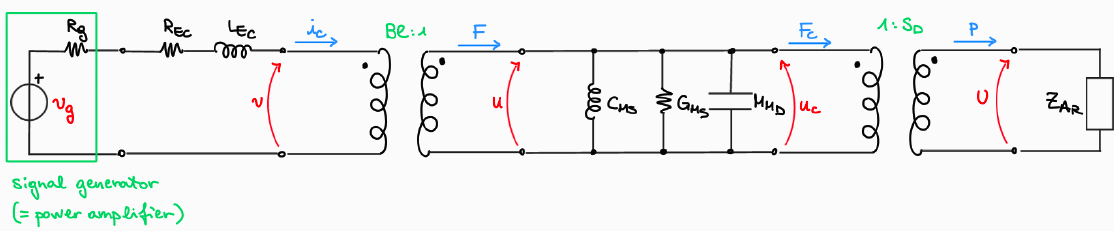
\includegraphics[width=0.75\textwidth]{electro_mech_acoustic_chain.png}
    \caption{Complete electrical-mechanical-acoustical chain of the loudspeaker. The power flow \(W_E \to W_M \to W_A\) is governed at each stage by the real part of the corresponding impedance; the reactive parts store and return energy without contributing to net radiation}
\end{figure}

    %! TEX root = main.tex

\graphicspath{{00_Images/06_chapter/}}

\chapter{Sound Radiation}
\label{ch:sound_radiation}

The previous chapter established how mean acoustic power depends on the real part of the acoustic radiation impedance. This chapter examines what that impedance actually looks like for the two fundamental idealized sources: the plane wave (an infinite, spatially uniform radiator) and the pulsating sphere (a compact omnidirectional source). It then applies the more realistic model of a rigid circular piston mounted in an infinite baffle, which closely approximates the behavior of a loudspeaker cone. The chapter concludes by showing that the air in front of the piston contributes a real, frequency-dependent mass load to the mechanical system, lowering the resonance frequency from the value that would be obtained in vacuum.

\section{Specific Acoustic Radiation Impedance}
\label{sc:61}

The specific acoustic impedance \(Z_s\) is defined as the ratio of acoustic pressure to particle velocity at a given point in the medium:
\begin{equation}
    Z_s = \frac{P}{u} = \frac{F/S}{U/S} = \frac{F}{U} \quad \left[\frac{\si{\pascal}}{\si{\meter\per\second}} = \si{\pascal\second\per\meter} = \text{Rayl}\right]
    \label{eq:specificImpedance}
\end{equation}
Unlike the acoustic impedance \(Z_A = P/U\) (which refers to volume velocity and has units of \(\si{\newton\second\per\meter\tothe{5}}\)), the specific impedance refers to particle velocity and carries units of Rayls. The two are related by \(Z_s = Z_A \cdot S\), where \(S\) is the relevant cross-sectional area. The mean acoustic intensity (power per unit area) is:
\[
\overline{I} = \frac{\overline{W_A}}{S} = \frac{P_\mathrm{RMS}^2}{\rho_0 c}
\]
where the last equality uses the plane-wave result \(Z_s = \rho_0 c\) derived below.

\subsection{Case 1: Plane Wave}
\label{ssc:611}

For a plane wave propagating in the positive \(x\)-direction, the pressure field is:
\[
p(x,t) = p_0 e^{j(\omega t - kx)}, \qquad k = \frac{\omega}{c} = \frac{2\pi f}{c} = \frac{2\pi}{\lambda}
\]
From the linearized Euler equation \(-\partial p/\partial x = \rho_0 \partial u/\partial t\), differentiating and solving for the particle velocity:
\[
u(x,t) = \frac{1}{c \rho_0} p(x,t)
\]
The specific acoustic impedance for a plane wave is therefore:
\begin{equation}
    Z_s = \frac{p}{u} = \rho_0 c \approx \SI{407}{\pascal\second\per\meter} \quad (\text{air at } \SI{20}{\degreeCelsius})
    \label{eq:planeWaveImpedance}
\end{equation}
This is a real constant, independent of frequency: for a plane wave, pressure and particle velocity are always in phase, the power factor is unity (\(\cos\beta = 1\)), and all supplied mechanical energy is radiated as propagating sound. There is no reactive part, so a plane wave source drives a purely resistive acoustic load. This is the ideal situation for a loudspeaker: if the radiation impedance were always purely resistive, the entire mechanical power delivered to the air would become radiated acoustic power.

\subsection{Case 2: Pulsating Sphere (Monopole)}
\label{ssc:612}

A pulsating sphere of radius \(R\) whose surface oscillates radially with particle velocity \(u_0\) radiates spherical waves. The volume velocity of the source is \(V_0 = 4\pi R^2 u_0\). The radiated pressure at the surface of the sphere is:
\[
|p(R)| = \frac{\rho_0 c V_0}{4\pi R}\cdot\frac{k}{\sqrt{1 + (kR)^2}}
\]
and the mean radiated power is:
\begin{equation}
    \overline{W_A} = S \rho_0 c u_{0,\mathrm{RMS}}^2\cdot\frac{(f/f_0)^2}{1 + (f/f_0)^2}, \qquad f_0 = \frac{c}{2\pi R}
    \label{eq:spherePower}
\end{equation}
where \(S = 4\pi R^2\) is the sphere surface area and \(f_0\) is a characteristic cutoff frequency determined by the sphere radius.

\begin{figure}[!htb]
    \centering
    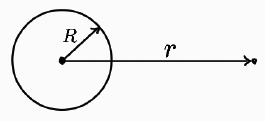
\includegraphics[width=0.45\textwidth]{monopole.png}
    \caption{Pulsating sphere (monopole) of radius \(R\). Sound radiation is omnidirectional and the radiated power depends on the ratio \(f/f_0\) where \(f_0 = c/(2\pi R)\)}
\end{figure}

\begin{figure}[!htb]
    \centering
    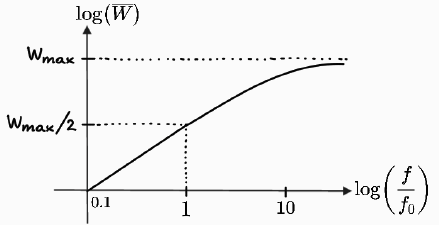
\includegraphics[width=0.50\textwidth]{log(W)(f).png}
    \caption{Mean radiated power \(\overline{W_A}\) of a pulsating sphere as a function of frequency on a logarithmic scale. Below the cutoff frequency \(f_0\), power falls as \(f^2\); above \(f_0\) it saturates at the plane-wave limit \(S\rho_0 c u_\mathrm{RMS}^2\)}
\end{figure}

The behavior of equation \eqref{eq:spherePower} has a clear physical interpretation. For \(f \gg f_0\) (i.e., \(kR \gg 1\), the sphere is large compared to the wavelength): \(\overline{W_A} \approx S \rho_0 c u_\mathrm{RMS}^2\), which is exactly the plane-wave result. The radiation is efficient and the specific impedance approaches the purely resistive value \(\rho_0 c\). For \(f \ll f_0\) (i.e., \(kR \ll 1\), the sphere is small compared to the wavelength): \(\overline{W_A} \propto (f/f_0)^2 \propto f^2\), so the radiated power falls off quadratically with decreasing frequency. In this regime the source is acoustically compact: the surrounding air is moved back and forth but the pressure perturbation cancels almost completely over the sphere's surface, and little net energy is radiated.

\paragraph{Physical meaning of the cutoff frequency} The frequency \(f_0 = c/(2\pi R)\) marks the transition between the mass-controlled regime (\(f \ll f_0\), reactive loading dominates) and the resistance-controlled regime (\(f \gg f_0\), efficient radiation). A critical consequence is that a source oscillating at zero frequency (\(f = 0\)) radiates zero acoustic power: steady motion of the surface merely displaces air without creating any propagating wave. Sound requires temporal variation of the source velocity; the faster the oscillation relative to \(f_0\), the more efficiently the source couples to the medium.
For a typical woofer with diaphragm radius \(a = \SI{10}{\centi\meter}\), the equivalent monopole cutoff frequency is \(f_0 = c/(2\pi a) \approx \SI{550}{\hertz}\). Below this frequency, the radiation resistance falls as \(f^2\) and the reactive (mass) part of the radiation impedance increasingly dominates the load seen by the diaphragm.

\section{Rigid Circular Piston in Infinite Baffle}
\label{sc:62}

A more accurate model for a real loudspeaker cone is the rigid circular piston of radius \(a\) mounted flush in an infinite, rigid, perfectly reflecting baffle. The baffle prevents rear-wave cancellation and constrains radiation to a half-space (\(2\pi\) steradians). This is also the reference geometry for which the radiation impedance is tabulated and against which real loudspeakers are often compared.

\begin{figure}[!htb]
    \centering
    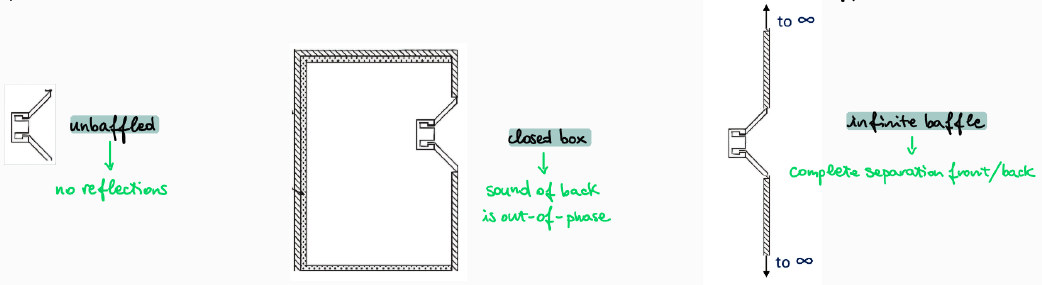
\includegraphics[width=0.65\textwidth]{rigid_piston_model.png}
    \caption{Rigid circular piston of radius \(a\) in an infinite baffle. The baffle prevents front-to-back acoustic short-circuiting, so radiation is restricted to the forward half-space. Different baffle configurations (infinite, finite, closed box) produce different radiation impedances and directivity patterns}
\end{figure}

\subsection{Far-Field Pressure and Directivity Function}
\label{ssc:621}

In the far field (\(r \gg a\)), the acoustic pressure radiated by the piston at a point \((r, \theta)\) in spherical coordinates is:
\[
\tilde{p}(r,\theta) = -j k a^2 \rho_0 c \tilde{u}_0 \frac{e^{-jkr}}{2r}\;D(\theta)
\]
where \(\tilde{u}_0\) is the complex piston velocity amplitude and \(D(\theta)\) is the directivity function:
\begin{equation}
    D(\theta) = \frac{2 J_1(ka\sin\theta)}{ka\sin\theta}
    \label{eq:directivity}
\end{equation}
Here \(J_1(\cdot)\) is the Bessel function of the first kind of order 1. On the axis (\(\theta = 0\)), \(D(0) = 1\) by the limit \(\lim_{x\to 0} 2J_1(x)/x = 1\), so the on-axis pressure is maximum and the expression simplifies to:
\[
\tilde{p}(r,0) = -j \rho_0 f \tilde{U}_0 \frac{e^{-jkr}}{2}, \qquad \tilde{U}_0 = \pi a^2 \tilde{u}_0
\]
where \(\tilde{U}_0\) is the volume velocity.

\subsection{The Parameter ka and Frequency-Dependent Behavior}
\label{ssc:622}

The dimensionless parameter \(ka\) controls all aspects of the piston's radiation:
\begin{equation}
    ka = \frac{2\pi a}{\lambda} = \frac{2\pi f a}{c} = \frac{f}{f_0}, \qquad f_0 = \frac{c}{2\pi a}
    \label{eq:ka}
\end{equation}
It expresses the ratio of the piston circumference \(2\pi a\) to the acoustic wavelength \(\lambda\), or equivalently the ratio of the operating frequency \(f\) to the characteristic frequency \(f_0\). The following table gives representative values of \(f_0\) for typical loudspeaker sizes:

\begin{table}[!htb]
\centering
\renewcommand{\arraystretch}{1.3}
\begin{tabular}{cc}
\hline
\textbf{Piston radius \(a\) (cm)} & \textbf{Cutoff frequency \(f_0\) (Hz)} \\
\hline
1  & 5500 \\
10 & 550  \\
30 & 183  \\
\hline
\end{tabular}
\caption{Characteristic cutoff frequency \(f_0 = c/(2\pi a)\) for three piston radii at \(c = \SI{343}{\meter\per\second}\)}
\end{table}

\paragraph{Low-frequency regime (\(ka \ll 1\))} When the piston diameter is much smaller than the wavelength, the Bessel function argument \(ka\sin\theta \ll 1\) for all angles, and \(D(\theta) \approx 1\) uniformly across the hemisphere: the radiation pattern is nearly omnidirectional. The source behaves as an acoustic monopole, and the radiated power falls as \(f^2\), exactly as for the pulsating sphere. The acoustic loading on the piston is predominantly reactive (mass-like), so the diaphragm is moving mostly against the inertia of the air rather than doing useful radiating work.

\begin{figure}[!htb]
    \centering
    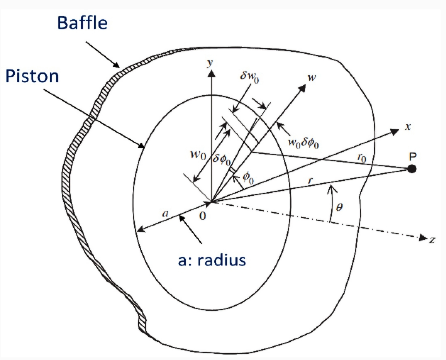
\includegraphics[width=0.45\textwidth]{rigid_piston.png}
    \caption{Rigid circular piston of radius \(a\) in an infinite baffle, showing the geometry for the far-field directivity calculation. The observation point P is at distance \(r\) and angle \(\theta\) from the piston axis}
\end{figure}

\paragraph{High-frequency regime (\(ka \gg 1\))} When the piston diameter is much larger than the wavelength, the zeros of \(J_1(ka\sin\theta)\) occur at angles progressively closer to the axis, and the radiation pattern narrows into a sharply focused main lobe along \(\theta = 0\) with increasingly numerous sidelobes at larger angles. In this regime the radiation resistance approaches the plane-wave value \(\rho_0 c\) and radiation is efficient, but it is concentrated in a narrow beam. From a practical standpoint, a large woofer operating at high frequencies radiates almost exclusively on-axis, causing severe high-frequency dispersion problems in the listening room.

\begin{figure}[!htb]
    \centering
    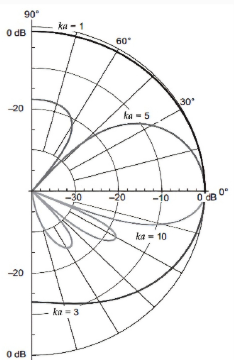
\includegraphics[width=0.40\textwidth]{directivity.png}
    \caption{Polar directivity pattern of a rigid circular piston for several values of \(ka\). For \(ka \ll 1\) the pattern is omnidirectional; as \(ka\) increases the radiation narrows into a progressively sharper main lobe with sidelobes}
\end{figure}

\subsection{Radiation Impedance of the Piston}
\label{ssc:623}

The specific radiation impedance seen by the piston surface is:
\begin{equation}
    Z_s = \frac{\tilde{F}}{\tilde{U}_0} = R_s + jX_s
    \label{eq:pistonImpedance}
\end{equation}
where the exact expressions in terms of Bessel and Struve functions are:
\[
R_s = \rho_0 c\left(1 - \frac{J_1(2ka)}{ka}\right), \qquad X_s = \rho_0 c \frac{\mathbf{H}_1(2ka)}{ka}
\]
with \(J_1(\cdot)\) the Bessel function of the first kind and \(\mathbf{H}_1(\cdot)\) the Struve function of the first kind. The mean acoustic power radiated by the piston is:
\[
\overline{W_A} = R_s S_D u_{0,\mathrm{RMS}}^2, \qquad S_D = \pi a^2
\]
For \(ka \ll 1\), the low-frequency asymptotic behavior of the radiation impedance components is:
\[
R_s \approx \frac{\rho_0}{2c} a^2 \omega^2 \propto \omega^2, \qquad X_s \approx \frac{8}{3\pi} a \rho_0 \omega \propto \omega
\]
The radiation resistance rises as \(\omega^2\) at low frequencies, confirming the \(f^2\) dependence of the radiated power for a velocity-driven piston. The radiation reactance rises as \(\omega\), behaving like the reactance of a mass \(M_{A1} = 8\rho_0 a/(3\pi^2)\) per unit area.

\begin{figure}[!htb]
    \centering
    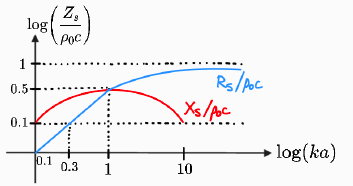
\includegraphics[width=0.75\textwidth]{acoustic_impedance_graph.png}
    \caption{Normalized specific radiation impedance \(Z_s/(\rho_0 c)\) for a rigid circular piston in an infinite baffle, plotted versus \(ka\) on a logarithmic scale. The resistive part \(R_s/(\rho_0 c)\) rises as \(\omega^2\) for \(ka \ll 1\) and saturates near unity for \(ka \gg 1\); the reactive part \(X_s/(\rho_0 c)\) rises as \(\omega\) for small \(ka\) and oscillates for large \(ka\)}
\end{figure}

\section{Acoustic End Correction: The Air Mass Load}
\label{sc:63}

The analysis of the piston's radiation impedance reveals that the reactive part \(X_s\), which rises linearly with frequency at low \(ka\), is equivalent to the reactance of an additional mass of air that must be accelerated every time the diaphragm moves. This air mass is not negligible: it represents a real physical contribution to the moving system of the loudspeaker that is not accounted for in the bare mechanical model of Chapter 4.

\subsection{The Acoustic End Correction Mass}
\label{ssc:631}

For a baffled piston at low frequencies (\(ka \ll 1\)), the reactive part of the radiation impedance per unit area is \(X_s = (8/3\pi) \rho_0 a \omega\). This is identical to the reactance of an acoustic mass:
\begin{equation}
    M_{A1} = \frac{8}{3\pi^2} \frac{\rho_0}{a} \quad \left[\si{\kilo\gram\per\meter\tothe{4}}\right]
    \label{eq:acousticMassA1}
\end{equation}
Referring this acoustic mass back to the mechanical domain through the diaphragm area \(S_D = \pi a^2\):
\begin{equation}
    M_{M1} = M_{A1} S_D^2 = \frac{8}{3\pi^2} \frac{\rho_0}{a}\cdot(\pi a^2)^2 = \frac{8\pi}{3} \rho_0 a^3 \approx 2.67 \rho_0 a^3 \quad [\si{\kilo\gram}]
    \label{eq:mechanicalEndCorrection}
\end{equation}
This result has a transparent geometric interpretation: \(M_{M1} = \rho_0\cdot\pi a^2\cdot(8a/3\pi) = \rho_0\cdot S_D\cdot(0.85 a)\), which is the mass of a column of air of cross-section \(S_D\) and effective length \(0.85 a\). The diaphragm does not move in isolation: it drags with it a cylinder of air whose length is approximately 85\% of the piston radius. This is the acoustic end correction, classically derived from potential flow theory.

\begin{figure}[!htb]
    \centering
    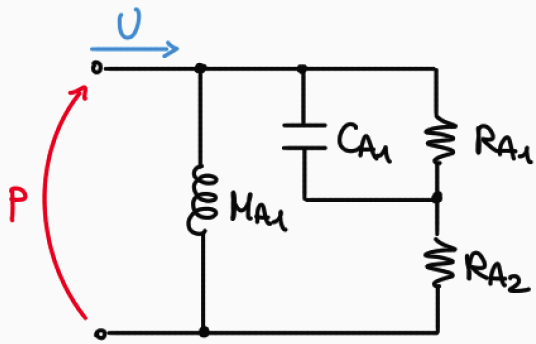
\includegraphics[width=0.65\textwidth]{radiation_circuit.png}
    \caption{Equivalent circuit at low frequencies showing the air mass \(M_{M1}\) in series with the radiation resistance \(R_{MR}\). The factor of 2 in the full expression \(2M_{M1}\) accounts for the air on both the front and rear faces of the loudspeaker when no baffle or enclosure is present}
\end{figure}

\subsection{Effect on the Total Moving Mass and Resonance Frequency}
\label{ssc:632}

The total moving mass of the loudspeaker system \(M_{MS}\) includes the diaphragm mass \(M_{MD}\) plus the air mass contributions from the front and rear radiation environments. For a loudspeaker mounted in an infinite baffle (open back), the front face carries an end correction \(M_{M1}\) and the rear face (which radiates into the enclosed air or free space behind the baffle) carries a second mass \(M_{M1}\), so:
\[
M_{MS} = M_{MD} + 2 M_{M1}
\]
For a driver in free air (no baffle at all), the same factor of 2 applies. In a closed-box enclosure, the rear air mass is modified by the acoustic compliance of the enclosure volume.
Since the air mass \(M_{M1} = 2.67 \rho_0 a^3\) scales with the cube of the piston radius, it becomes increasingly significant for larger drivers. For a \SI{10}{\centi\meter} radius woofer:
\[
M_{M1} = 2.67 \times \SI{1.2}{\kilo\gram\per\cubic\meter} \times (\SI{0.1}{\meter})^3 \approx \SI{3.2}{\gram}
\]
This value is comparable to the diaphragm mass of a typical woofer (5 to 15 grams), so the air mass correction is not a minor perturbation but a substantial fraction of the total moving mass.
The consequence for the system resonance frequency is direct. From Chapter 4, the free-air resonance frequency in the absence of any radiation load is:
\[
f_{s,\mathrm{bare}} = \frac{1}{2\pi\sqrt{M_{MD} C_{MS}}}
\]
When the air mass is included, the effective moving mass increases and the resonance frequency drops:
\begin{equation}
    f_s = \frac{1}{2\pi\sqrt{M_{MS} C_{MS}}} = \frac{1}{2\pi\sqrt{(M_{MD} + 2M_{M1}) C_{MS}}} < f_{s,\mathrm{bare}}
    \label{eq:resonanceWithAirMass}
\end{equation}
The parameter \(f_s\) measured on a physical loudspeaker (for instance from the impedance peak) already includes the air mass contribution, so it directly yields \(M_{MS}\) rather than the bare diaphragm mass \(M_{MD}\). When Thiele-Small parameters are extracted from impedance measurements, the quoted \(M_{MS}\) is the total moving mass including the air load.

\begin{figure}[!htb]
    \centering
    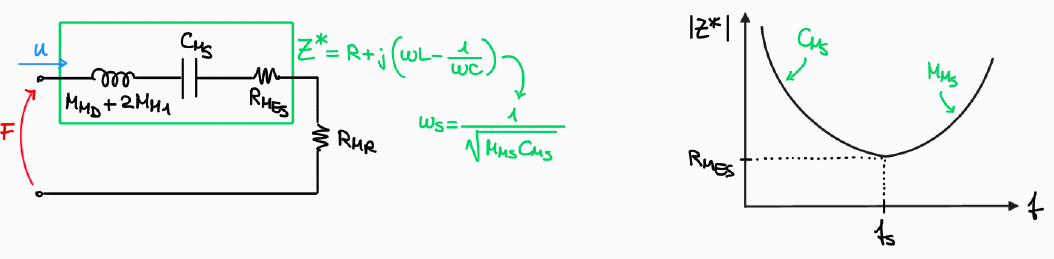
\includegraphics[width=0.80\textwidth]{low_freq_equiv.png}
    \caption{Low-frequency equivalent circuit of the loudspeaker including the air mass \(M_{M1}\). The total moving mass \(M_{MS} = M_{MD} + 2M_{M1}\) determines the resonance frequency \(f_s\) of the complete system. The radiation resistance \(R_{MR} \propto \omega^2\) rises steeply at low frequencies and falls far below the suspension damping \(R_{MS}\) at the resonance frequency of most practical woofers}
\end{figure}

\paragraph{Physical picture} The air in front of the cone is not acoustically transparent. When the diaphragm moves forward, it must accelerate a plug of air of finite mass before that mass can propagate its displacement outward as a sound wave. At low frequencies this plug moves back and forth with the cone but radiates very little power (because \(R_s \propto \omega^2\) is small), behaving as a purely inertial load. At frequencies above \(f_0 = c/(2\pi a)\), the air plug can no longer keep up with the cone and begins to decouple: the radiation resistance rises toward \(\rho_0 c\) and efficient sound radiation begins. The loudspeaker designer must therefore choose the diaphragm radius and resonance frequency such that the operating bandwidth falls in the transition region where radiation is efficient but directivity is not yet excessive.

    %! TEX root = main.tex

\graphicspath{{00_Images/07_chapter/}}

\chapter{Loudspeaker Dynamics and Resonance}
\label{ch:dynamics}

The complete mechanical section of the loudspeaker, established in the previous chapters, can now be analyzed as a resonant system driven by an electrical source.
The interplay between the suspension compliance and the diaphragm mass produces a mechanical resonance at the fundamental frequency \(f_s\); the quality factor of this resonance governs the shape of the impedance peak, the diaphragm velocity, displacement, and acceleration across the audio band.
This chapter derives the resonance and quality-factor expressions from the equivalent circuit, then traces the frequency-dependent behavior of all three kinematic quantities.

\section{RLC Resonant System}
\label{sc:71}

The mechanical section of the loudspeaker is a second-order resonant system.
Under the admittance analogy, the diaphragm mass \(M_{MS}\), suspension compliance \(C_{MS}\), and total mechanical resistance \(R_M = R_{ME} + R_{MS} + R_{MR}\) form a parallel RLC network in which velocity \(u_C\) plays the role of voltage and force \(F_C\) plays the role of current.
Under the impedance analogy, the same three elements form a series RLC network in which velocity is the shared current and the driving force is the loop voltage.
Both representations are physically equivalent and produce identical predictions once all quantities are referred to the same domain.

\begin{figure}[!htb]
    \centering
    \subfloat[Parallel RLC (admittance analogy)]{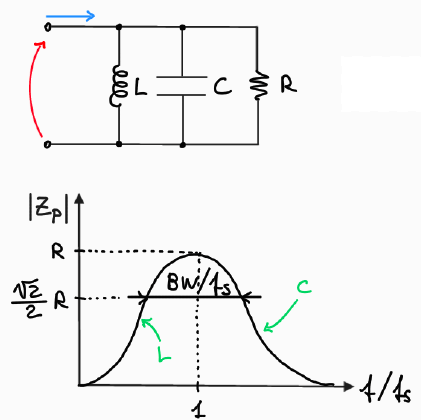
\includegraphics[width=0.50\linewidth]{parallel_RLC_with_Q.png}}
    \\
    \subfloat[Series RLC (impedance analogy)]{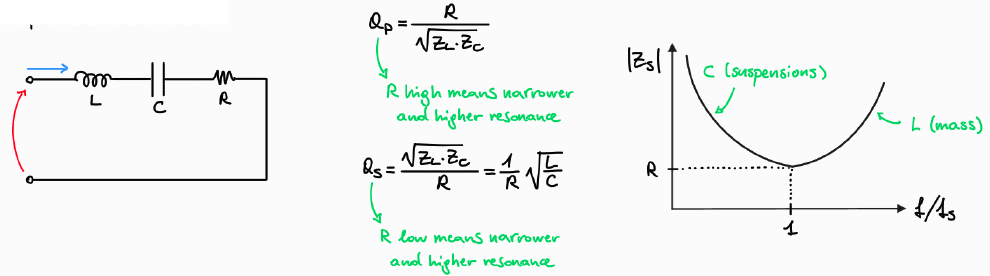
\includegraphics[width=0.85\linewidth]{parallel_to_series_RLC.png}}
    \caption{The mechanical section of the loudspeaker modeled as a parallel RLC resonator (admittance analogy, left) and as a series RLC resonator (impedance analogy, right). The resonance frequency \(f_s\) and the quality factor \(Q\) are identical in both representations; only the circuit topology differs}
\end{figure}

\subsection{Resonance Frequency}
\label{ssc:711}

The resonance condition is reached when the inductive and capacitive reactances cancel.
For the parallel network (admittance analogy), this occurs at:
\[
\omega_s L_{ES} = \frac{1}{\omega_s C_{ED}}
\qquad\Longrightarrow\qquad
\omega_s = \frac{1}{\sqrt{L_{ES} C_{ED}}}
\]
Substituting the electrical equivalents \(L_{ES} = (Bl)^2 C_{MS}\) and \(C_{ED} = M_{MS}/(Bl)^2\):
\[
\omega_s = \frac{1}{\sqrt{(Bl)^2 C_{MS} \cdot M_{MS}/(Bl)^2}} = \frac{1}{\sqrt{M_{MS} C_{MS}}}
\]
The \(Bl\) factor cancels exactly, confirming that the resonance frequency is a purely mechanical parameter, independent of the electromagnetic coupling:
\begin{equation}
    f_s = \frac{1}{2\pi\sqrt{M_{MS} C_{MS}}}
    \label{eq:resonanceFrequency}
\end{equation}
At \(f = f_s\), the impedance of the parallel RLC reaches its maximum value \(R_{ES}\), the circuit behaves as a pure resistance, and the diaphragm velocity peaks at its maximum amplitude.
The bandwidth of the resonance peak, measured between the two frequencies \(f_H\) and \(f_L\) at which the impedance magnitude falls to \(1/\sqrt{2}\) of its maximum, is:
\[
Q = \frac{f_s}{f_H - f_L}
\]

\begin{figure}[!htb]
    \centering
    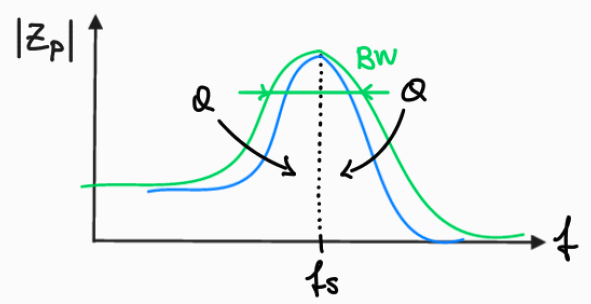
\includegraphics[width=0.50\linewidth]{Q_Factor_Graph.png}
    \caption{Influence of the quality factor \(Q\) on the magnitude response \(|Z_P(f)|\) of the parallel RLC. A higher \(Q\) produces a sharper resonance peak and a narrower bandwidth \(f_H - f_L\)}
\end{figure}

For the parallel RLC with resistance \(R\), inductance \(L\), and capacitance \(C\), the normalized impedance expression is:
\[
Z_P = R \frac{j\dfrac{1}{Q}\dfrac{f}{f_s}}{1 - \left(\dfrac{f}{f_s}\right)^2 + j\dfrac{1}{Q}\dfrac{f}{f_s}}
\]
where \(Q = R\sqrt{C/L}\).

\paragraph{Multiple RLC contributions} When the radiation resistance \(R_{MR}\) and the referred electrical resistance \(R_{ME}\) both appear alongside the suspension resistance \(R_{MS}\), the total mechanical resistance is their sum \(R_M = R_{ME} + R_{MS} + R_{MR}\).
Each contributes an independent quality factor, and the effective \(Q\) is controlled by the smallest individual contribution, in direct analogy with the parallel combination of resistors.

\begin{figure}[!htb]
    \centering
    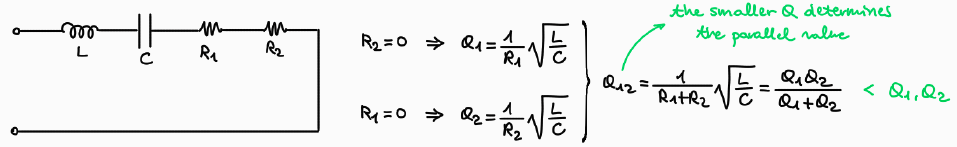
\includegraphics[width=0.85\linewidth]{multi_RLC_hint.png}
    \caption{Multiple RLC contributions to the mechanical branch. Each resistance defines its own quality factor; the effective parallel \(Q\) is dominated by the branch with the lowest \(Q\), i.e., the highest damping contribution}
\end{figure}

\section{Q-Factor Combination}
\label{sc:72}

The total damping of the loudspeaker system is quantified by the total quality factor \(Q_{TS}\), which collects both the mechanical losses in the suspension and the electromagnetic losses due to current flowing through the voice-coil circuit.

\subsection{Mechanical Quality Factor}
\label{ssc:721}

The mechanical quality factor \(Q_{MS}\) measures the sharpness of the resonance produced by the suspension damping alone, in the absence of any electromagnetic loading.
It is defined as:
\[
Q_{MS} = \frac{1}{R_{MS}}\sqrt{\frac{M_{MS}}{C_{MS}}}
\]
A high \(Q_{MS}\) corresponds to a lightly damped suspension and a sharp impedance peak; a low \(Q_{MS}\) indicates heavy mechanical losses that broaden the resonance.

\subsection{Electrical Quality Factor}
\label{ssc:722}

The electrical quality factor \(Q_{ES}\) captures the damping contributed by the electromagnetic coupling between the voice coil and the external electrical circuit.
The referred electrical resistance is \(R_{ME} = (Bl)^2/(R_g + R_{EC})\), so:
\[
Q_{ES} = \frac{1}{R_{ME}}\sqrt{\frac{M_{MS}}{C_{MS}}} = \frac{R_g + R_{EC}}{(Bl)^2}\sqrt{\frac{M_{MS}}{C_{MS}}}
\]
A stronger magnetic circuit (larger \(Bl\)) or a lower source resistance both reduce \(Q_{ES}\), increasing electromagnetic damping.
This is the physical mechanism by which amplifier output impedance affects the loudspeaker's transient response.

\subsection{Total Quality Factor}
\label{ssc:723}

Since \(R_{ME}\) and \(R_{MS}\) appear as additive resistances in the total mechanical resistance, their conductances add in the admittance representation.
This yields:
\[
\frac{1}{Q_{TS}} = \frac{1}{Q_{ES}} + \frac{1}{Q_{MS}}
\]
Solving for \(Q_{TS}\):
\begin{equation}
    Q_{TS} = \frac{Q_{ES} Q_{MS}}{Q_{ES} + Q_{MS}}
    \label{eq:Qts}
\end{equation}
This expression is formally identical to the formula for two resistors in parallel: the total quality factor is the harmonic combination of the mechanical and electrical contributions.
The smaller of the two individual quality factors dominates the result; increasing electromagnetic damping (reducing \(Q_{ES}\)) lowers \(Q_{TS}\) even when the suspension is lightly damped.

\section{Displacement, Velocity, and Acceleration}
\label{sc:73}

With the mechanical network fully characterized, the kinematic response of the diaphragm-voice coil assembly as a function of frequency can be derived.
The normalized frequency variable is \(f/f_s\), and the complete behavior is governed by three transfer functions: \(\beta_C(f)\) for velocity, \(\gamma_C(f)\) for displacement, and \(\alpha_C(f)\) for acceleration.

\begin{figure}[!htb]
    \centering
    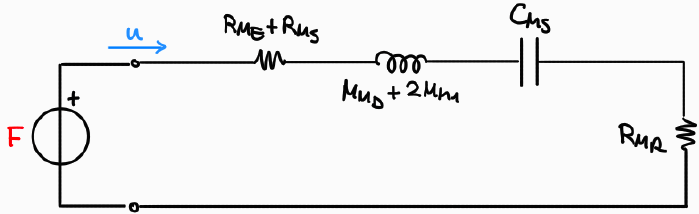
\includegraphics[width=0.60\linewidth]{high_freq_circuit.png}
    \caption{Complete mechanical equivalent circuit for the derivation of the kinematic transfer functions. The voice-coil driving force \(F = Bl i_c\) excites the series combination of the total mechanical resistance \(R_M\), the moving mass \(M_{MS}\), and the suspension compliance \(C_{MS}\)}
    \label{fig:highFreqCircuit}
\end{figure}

\subsection{Voice-Coil Velocity}
\label{ssc:731}

Starting from the driving force \(F_\mathrm{RMS} = Bl v_g/(R_g + R_{EC})\) and the total mechanical impedance \(Z_M\), the voice-coil velocity is:
\[
u_C = \frac{F}{Z_M} = \frac{v_g}{Bl} \frac{1}{Q_{ES}} \beta_C(f)
\]
where the normalized velocity transfer function is:
\begin{equation}
    \beta_C(f) = \frac{j\dfrac{f}{f_s}}{1 - \left(\dfrac{f}{f_s}\right)^2 + j\dfrac{1}{Q_{TS}}\dfrac{f}{f_s}}
    \label{eq:betaC}
\end{equation}
The magnitude \(|\beta_C|\) peaks at \(f = f_s\) with value \(Q_{TS}\), rising as \(f/f_s\) below resonance and falling as \(f_s/f\) above it.

\begin{figure}[!htb]
    \centering
    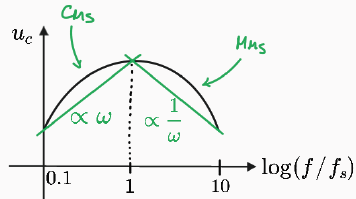
\includegraphics[width=0.60\linewidth]{u_c(f).png}
    \caption{Normalized voice-coil velocity \(|u_C|\) as a function of \(\log(f/f_s)\). The velocity rises as \(f\) in the stiffness-controlled region, peaks at resonance, then decays as \(1/f\) in the mass-controlled region above \(f_s\)}
\end{figure}

\subsection{Diaphragm Displacement}
\label{ssc:732}

Displacement is the time integral of velocity, so in the sinusoidal regime \(x_C = u_C/(j\omega)\):
\[
x_C = \frac{v_g}{Bl} \frac{1}{Q_{ES}} \frac{1}{2\pi f_s} \gamma_C(f)
\]
where the normalized displacement transfer function is:
\begin{equation}
    \gamma_C(f) = \frac{1}{1 - \left(\dfrac{f}{f_s}\right)^2 + j\dfrac{1}{Q_{TS}}\dfrac{f}{f_s}}
    \label{eq:gammaC}
\end{equation}
Below resonance, where the compliance dominates, \(\gamma_C \approx 1\) and the displacement is constant, equal to \(F C_{MS}\): the cone moves like a spring-loaded body with excursion set entirely by the suspension stiffness.
This is the stiffness-controlled regime.

\begin{figure}[!htb]
    \centering
    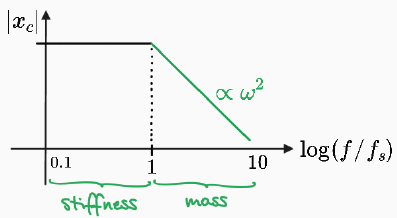
\includegraphics[width=0.60\linewidth]{x_c(f).png}
    \caption{Normalized diaphragm displacement \(|x_C|\) as a function of \(\log(f/f_s)\). Below \(f_s\) the displacement is constant (stiffness-controlled); at resonance it peaks by a factor \(Q_{TS}\); above \(f_s\) it falls as \(1/f^2\) in the mass-controlled region}
\end{figure}

\subsection{Diaphragm Acceleration and the Mass-Controlled Regime}
\label{ssc:733}

Acceleration is the time derivative of velocity, so \(a_C = j\omega u_C\):
\[
a_C = \frac{v_g}{R_g + R_{EC}} \frac{Bl}{M_{MS}} \alpha_C(f)
\]
where the normalized acceleration transfer function is:
\begin{equation}
    \alpha_C(f) = \frac{-\left(\dfrac{f}{f_s}\right)^2}{1 - \left(\dfrac{f}{f_s}\right)^2 + j\dfrac{1}{Q_{TS}}\dfrac{f}{f_s}}
    \label{eq:alphaC}
\end{equation}

\begin{figure}[!htb]
    \centering
    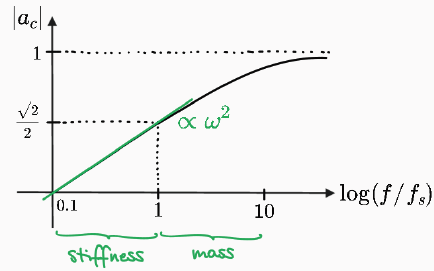
\includegraphics[width=0.60\linewidth]{a_c(f).png}
    \caption{Normalized diaphragm acceleration \(|a_C|\) as a function of \(\log(f/f_s)\). The acceleration rises as \(f^2\) below resonance, peaks at \(f_s\), then becomes constant in the mass-controlled region above \(f_s\). Since far-field pressure is proportional to acceleration, this plateau corresponds to a flat acoustic pressure response}
\end{figure}

\paragraph{The mass-controlled plateau} Above resonance, where \(f \gg f_s\), the inertial term \(\omega M_{MS}\) dominates the mechanical impedance and \(\alpha_C(f) \to -1\), so:
\[
a_C \approx \frac{v_g}{R_g + R_{EC}} \frac{Bl}{M_{MS}} = \text{const}
\]
The acceleration is independent of frequency, depending only on the ratio \(Bl/M_{MS}\) and the source voltage.
Correspondingly, the velocity decays as \(u_C \propto 1/f\) and the displacement falls as \(x_C \propto 1/f^2\), so cone excursion at high frequencies is naturally suppressed.
The far-field acoustic pressure, being proportional to diaphragm acceleration, is therefore flat above \(f_s\): this is the design target for a broadband loudspeaker, and it explains why the mass-controlled region is the primary operating band of a woofer.

    %! TEX root = main.tex

\graphicspath{{00_Images/08_chapter/}}

\chapter{Flat Power, Efficiency, and Thiele-Small Parameters}
\label{ch:efficiency}

The previous chapter showed that above resonance the diaphragm acceleration is constant, independent of frequency.
This chapter traces the consequence of that result for the radiated acoustic power, derives the efficiency of the electrodynamic loudspeaker as a complete transducer, and introduces the compact set of parameters needed to characterize any driver independently of the specific equivalent circuit used during analysis.

\section{Frequency-Independent Acoustic Power}
\label{sc:81}

The mean acoustic power radiated by the loudspeaker in the band above resonance is:
\[
\overline{W_A} = R_{MR} u_{C,\mathrm{RMS}}^2
\]
where \(R_{MR} = S_D^2 R_{AR}\) is the mechanical radiation resistance and \(u_C\) is the diaphragm velocity.
At first glance, since \(u_C \propto 1/f\) in the mass-controlled regime, one might expect \(\overline{W_A} \propto 1/f^2\), implying a steadily decreasing radiated power.
However, the radiation resistance is not constant: as shown in chapter \ref{ch:sound_radiation}, for a piston with \(ka \ll 1\) the specific radiation resistance rises as:
\[
R_s \approx \frac{a^2 \rho_0}{2c} \omega^2 \propto \omega^2
\]
Referring this to the mechanical domain, \(R_{MR} = S_D R_s \propto \omega^2\).
The two frequency dependences cancel exactly:
\[
\overline{W_A} = R_{MR} u_{C,\mathrm{RMS}}^2 \propto \omega^2 \cdot \frac{1}{\omega^2} = \text{const}
\]
Substituting the explicit expressions for \(u_C\) in the mass-controlled regime and for \(R_{MR}\) in the low-frequency limit:
\begin{equation}
    \overline{W_A} = \frac{v_{g,\mathrm{RMS}}^2 (Bl)^2 S_D^2 \rho_0}{(R_g + R_{EC})^2 \pi c M_{MS}^2}
    \label{eq:flatPower}
\end{equation}
This result is remarkable: the radiated acoustic power is independent of frequency for all \(f\) in the range \(f_s < f < f_0\), where \(f_0 = c/(2\pi a)\) is the piston cutoff frequency.
The physical picture is that, while the diaphragm moves with diminishing velocity as frequency rises, it simultaneously becomes a better radiator because its size grows relative to the shrinking wavelength.
The two effects balance with arithmetic precision, maintaining a constant acoustic output.
The design implication is direct: to obtain a flat acoustic power response over a given bandwidth, the working range of the driver must lie within the interval \(f_s < f < f_0\), making the choice of \(f_s\) and diaphragm radius \(a\) the two primary design variables.

\section{Loudspeaker Efficiency}
\label{sc:82}

The electroacoustic efficiency \(\varepsilon\) of the loudspeaker is defined as the ratio of the mean radiated acoustic power to the mean electrical power absorbed from the source:
\[
\varepsilon = \frac{\overline{W_A}}{\overline{W_E}}
\]
The mean electrical power delivered to the loudspeaker terminals is approximately \(\overline{W_E} \approx v_{g,\mathrm{RMS}}^2/R_{EC}\), assuming the source resistance is negligible compared to the voice-coil resistance (\(R_g \ll R_{EC}\)).
Dividing equation \eqref{eq:flatPower} by this expression:
\begin{equation}
    \varepsilon = \frac{(Bl)^2 \rho_0}{\pi c R_{EC}}\left(\frac{S_D}{M_{MS}}\right)^2
    \label{eq:efficiency}
\end{equation}
Equation \eqref{eq:efficiency} reveals the three principal levers available to the designer for improving efficiency: increasing the force factor \(Bl\) (stronger magnet, more wire in the gap), reducing the voice-coil resistance \(R_{EC}\), and maximizing the ratio \(S_D/M_{MS}\) (large, lightweight diaphragm).

\paragraph{Numerical example} Inserting typical values for a commercial woofer:
\[
Bl = \SI{10}{\newton\per\ampere}, \quad
R_{EC} = \SI{6}{\ohm}, \quad
S_D = \pi (0.1)^2 \approx \SI{0.03}{\meter\squared}
\]
\[
M_{MS} = M_{MD} + 2M_{M1} = 0.1 + 0.006 \approx \SI{0.2}{\kilo\gram}, \quad
\rho_0 = \SI{1.2}{\kilo\gram\per\cubic\meter}, \quad
c = \SI{343}{\meter\per\second}
\]
the efficiency evaluates to:
\[
\varepsilon \approx 0.15\%
\]
Less than two thousandths of the electrical energy supplied by the amplifier is converted into radiated sound; the remainder is dissipated as heat in the voice coil, the suspension, and the magnetic circuit.
This extraordinarily low efficiency is not a design failure but a fundamental consequence of the large impedance mismatch between the stiff, heavy mechanical system and the compliant, light acoustic medium.
Despite this, the electrodynamic loudspeaker remains the dominant transducer technology because its efficiency, though low in absolute terms, is achievable at high power levels with good linearity and in a compact, reproducible form.

\begin{figure}[!htb]
    \centering
    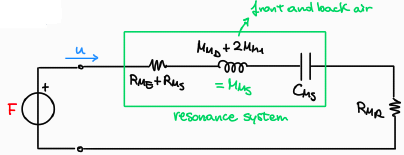
\includegraphics[width=0.60\linewidth]{loudspeaker_elec_scheme.png}
    \caption{Complete equivalent circuit of the loudspeaker at low-to-mid frequencies, referred to the electrical domain. The efficiency \(\varepsilon \approx 0.15\%\) follows from the ratio of the radiation resistance element to the total electrical losses}
\end{figure}

\section{The Thiele-Small Parameters}
\label{sc:83}

Any two engineers who measure the same loudspeaker must obtain the same small-signal behavior, regardless of which equivalent circuit model or which analogy they prefer.
This requirement motivates a compact, model-independent set of measurable parameters that fully characterize the driver near resonance.
The Thiele-Small parameter set, developed by Neville Thiele and Richard Small in the early 1970s, has become the universal standard in loudspeaker datasheets.
Six fundamental parameters are sufficient to reconstruct all elements of the equivalent circuit and to predict the in-box frequency response:

\begin{itemize}
    \item \(R_{EC}\): the DC resistance of the voice coil, measured in \si{\ohm}.
    \item \(Q_{ES}\): the electrical quality factor, quantifying the electromagnetic damping at resonance.
    \item \(Q_{MS}\): the mechanical quality factor, quantifying the suspension damping at resonance.
    \item \(f_s\): the free-air fundamental resonance frequency, in \si{\hertz}, given by equation \eqref{eq:resonanceFrequency}.
    \item \(S_D\): the effective piston area of the diaphragm, in \si{\meter\squared}, typically approximated as the area enclosed by the midpoint of the surround.
    \item \(V_{AS}\): the equivalent suspension volume, in \si{\meter\cubed} or liters, defined below.
\end{itemize}

From these six quantities, all derived parameters follow algebraically:
\[
C_{MS} = \frac{V_{AS}}{S_D^2 \rho_0 c^2}, \qquad
M_{MS} = \frac{1}{(2\pi f_s)^2 C_{MS}}, \qquad
R_{MS} = \frac{1}{Q_{MS}}\sqrt{\frac{M_{MS}}{C_{MS}}}
\]
\[
Bl = \sqrt{\frac{R_{EC}}{2\pi f_s Q_{ES} C_{MS}}}, \qquad
Q_{TS} = \frac{Q_{ES} Q_{MS}}{Q_{ES} + Q_{MS}}
\]

\section{Equivalent Suspension Volume}
\label{sc:84}

The equivalent suspension volume \(V_{AS}\) is the parameter that links the mechanical compliance of the suspension to a volume of air, making it directly comparable to enclosure volumes in box design.

\subsection{Physical Definition}
\label{ssc:841}

The acoustic compliance of a rigid sealed volume \(V_0\) of air undergoing adiabatic compression is:
\[
C_A = \frac{V_0}{\gamma P_0} \approx \frac{V_0}{\rho_0 c^2}
\]
where \(\gamma \approx 1.4\) is the ratio of specific heats and \(P_0\) is the ambient pressure.
The mechanical compliance \(C_{MS}\) of the suspension, when referred to the acoustic domain through the diaphragm area, defines an equivalent acoustic compliance:
\[
C_{AS} = {C_{MS}}{S_D^{2}}
\]
Setting this equal to \(C_A\) and solving for the volume:
\begin{equation}
    V_{AS} = C_{AS} \rho_0 c^2 = C_{MS} S_D^2 \rho_0 c^2
    \label{eq:VAS}
\end{equation}
The parameter \(V_{AS}\) is therefore the volume of air that, when sealed in a rigid container and compressed adiabatically, presents exactly the same acoustic compliance as the loudspeaker suspension.
Numerically, a woofer with a soft suspension and a large diaphragm can have \(V_{AS}\) of tens or even hundreds of liters; a tweeter with a stiff diaphragm typically has \(V_{AS}\) below one liter.

\subsection{The Syringe Analogy}
\label{ssc:842}

The concept of acoustic compliance as an air spring is most vividly demonstrated by a simple experiment: consider a medical syringe with its opening sealed by a thumb.
When the plunger is pushed inward, the trapped air is compressed and a restoring pressure builds up proportionally to the displacement, exactly as a mechanical spring restores a displaced mass.
Releasing the plunger, the compressed air pushes it back to its original position.
The analogy with a loudspeaker enclosure is direct: the volume of air sealed inside a closed-box cabinet plays the same role as the syringe volume.
The box air acts as an additional spring in series with the suspension, stiffening the total compliance and raising the resonance frequency above the free-air value \(f_s\).
The smaller the enclosure volume \(V_B\) relative to \(V_{AS}\), the stiffer the air spring and the greater the upward shift in resonance.
The ratio \(V_{AS}/V_B\) therefore quantifies how much the enclosure loads the suspension, and \(V_{AS}\) itself is the natural reference volume for enclosure design: a box of volume \(V_B = V_{AS}\) doubles the total stiffness, raising the resonance frequency by a factor of \(\sqrt{2}\).
More generally, the closed-box resonance frequency is:
\[
f_c = f_s \sqrt{1 + \frac{V_{AS}}{V_B}}
\]
This relation, together with equation \eqref{eq:Qts} and the known \(Q_{TS}\), allows the entire in-box frequency response to be predicted from the six Thiele-Small parameters before any physical enclosure is built.
The compactness and universality of the Thiele-Small framework account for its adoption as the standard specification language for the entire loudspeaker industry.

    %! TEX root = main.tex

\graphicspath{{00_Images/09_chapter/}}

\chapter{Loudspeaker Systems and Enclosures}
\label{ch:enclosures}

The bare electrodynamic driver analyzed in the preceding chapters radiates from both its front and rear faces simultaneously.
At low frequencies, where the acoustic wavelength is much larger than the diaphragm diameter, the two radiating surfaces are close enough that their contributions interfere destructively in the far field, severely limiting bass output.
The enclosure solves this fundamental problem by controlling the acoustic environment seen by the rear face of the diaphragm, allowing the front radiation to proceed unimpeded.
This chapter examines three enclosure topologies in order of increasing acoustic complexity: the unbaffled driver, the closed box, and the vented (bass-reflex) box.

\section{Unbaffled and Baffled Loudspeakers}
\label{sc:91}

\subsection{The Unbaffled Driver as a Dipole Source}
\label{ssc:911}

When a loudspeaker operates without any baffle, the diaphragm faces air on both sides.
The front face produces a positive pressure increment when it moves forward, while the rear face simultaneously produces a negative pressure increment of equal magnitude in the backward direction.
In the far field, these two contributions from a source of finite extent but vanishing dipole separation (relative to the wavelength at low frequencies) interfere destructively: air displaced forward is immediately replenished by air drawn around the driver from behind, so no net volume velocity is injected into the medium.
This effect is known as acoustic short-circuiting, and it makes the unbaffled driver behave as a dipole source rather than a monopole.
The far-field pressure of a dipole source depends on frequency, distance, and direction of observation as:
\[
p \propto \frac{f^2 U_0}{r} \cos\theta
\]
where \(U_0 = \pi a^2 u_c\) is the volume velocity, \(r\) is the observation distance, and \(\theta\) is the angle measured from the diaphragm axis.
The \(\cos\theta\) factor produces a figure-eight polar pattern: maximum sensitivity on axis (\(\theta = 0\)), zero sensitivity in the plane of the diaphragm (\(\theta = \pm 90°\)).

\paragraph{Frequency response below \(f_s\): stiffness-controlled} Below the mechanical resonance frequency, the suspension compliance dominates the impedance and the diaphragm velocity is \(u_c \propto f\), so \(U_0 \propto f\).
Substituting into the dipole pressure formula:
\[
p \propto f^2 \cdot f = f^3
\]
The pressure rises at \(+18 \mathrm{dB/oct}\) as frequency increases, or equivalently falls at \(18 \mathrm{dB/oct}\) below the stiffness-controlled cutoff.
This extremely steep rolloff makes the unbaffled driver impractical for bass reproduction.

\paragraph{Frequency response above \(f_s\): mass-controlled} Above resonance, the diaphragm mass dominates and \(u_c \propto 1/f\), so \(U_0 \propto 1/f\).
The far-field pressure then scales as:
\[
p \propto f^2 \cdot \frac{1}{f} = f
\]
Even in the mass-controlled region, the pressure still rises at \(+6 \mathrm{dB/oct}\) with increasing frequency: there is no flat passband.
This means an unbaffled driver can never achieve a constant SPL response without equalization, and the limited practical interest of the unbaffled configuration is mainly restricted to open-baffle designs used for specific aesthetic or spatial reasons.

\subsection{Baffle Configurations}
\label{ssc:912}

The fundamental purpose of any baffle or enclosure is to prevent the rear acoustic wave from canceling the front radiation.
Three idealized configurations are commonly distinguished.

\begin{figure}[!htb]
    \centering
    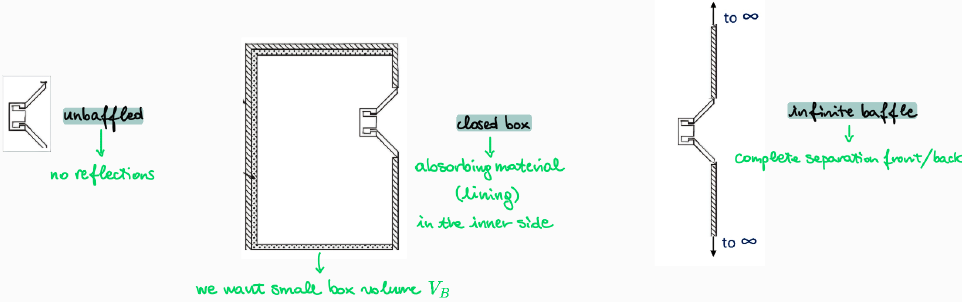
\includegraphics[width=0.80\textwidth]{baffle_configurations.png}
    \caption{Comparison of baffle configurations: unbaffled driver (left), closed-box baffle (center), and infinite baffle (right). The closed box approximates the infinite baffle in practice by enclosing the rear radiation in a sealed cabinet}
\end{figure}

The infinite baffle is the idealized case of a rigid wall of infinite extent in which the driver is mounted flush: front and rear radiation are completely separated.
The infinite baffle presents the piston radiation impedance derived in chapter \ref{ch:sound_radiation} on the front side, and zero acoustic loading on the rear.
It is not physically realizable but serves as the reference against which all practical designs are assessed.
The closed-box (sealed) baffle approximates the infinite baffle by enclosing the rear of the driver in a rigid cabinet.
The enclosed air volume introduces an additional acoustic compliance that stiffens the suspension and raises the resonance frequency, as analyzed in section \ref{sc:92}.
The vented (bass-reflex) box replaces the sealed rear panel with a tuned acoustic port, adding a second resonator that extends the usable bass response at the cost of a steeper rolloff below the system cutoff, as analyzed in section \ref{sc:93}.

\begin{figure}[!htb]
    \centering
    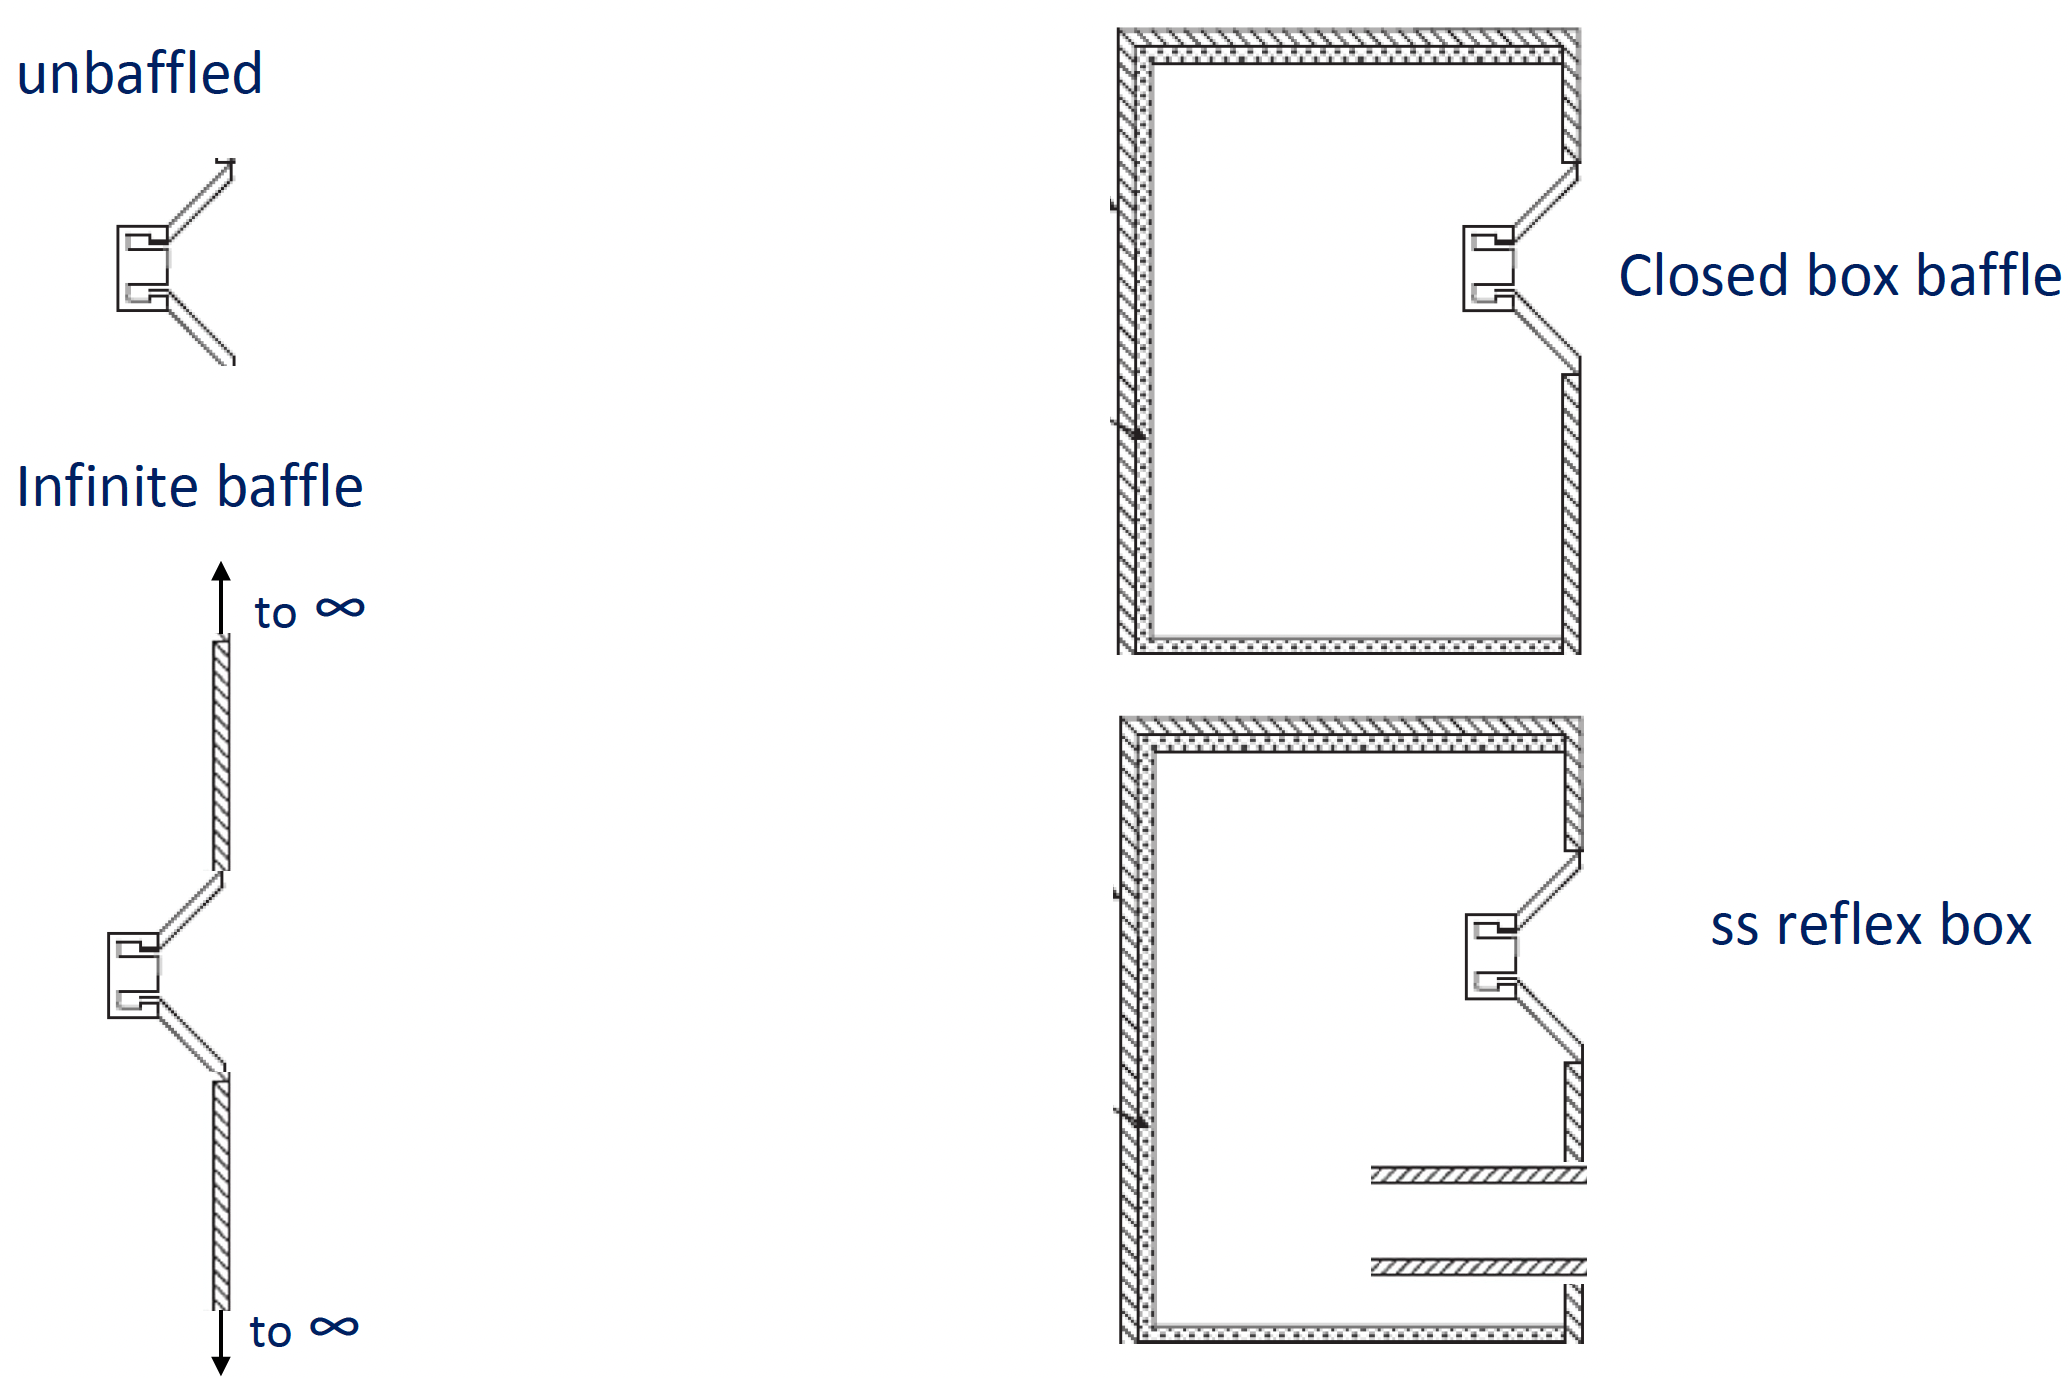
\includegraphics[width=0.70\textwidth]{baffle_types.png}
    \caption{Representative physical realizations of the three baffle topologies: open-baffle panel (left), sealed cabinet (center), and vented cabinet with front-mounted port (right)}
\end{figure}

\section{The Closed-Box Enclosure}
\label{sc:92}

The closed-box (sealed-cabinet) enclosure is the simplest practical enclosure topology.
The cabinet is made acoustically rigid, and the rear of the driver sees a sealed air volume \(V_B\).
The enclosed air behaves as an acoustic compliance:
\[
C_{AB} = \frac{V_B}{\rho_0 c^2}
\]
this is an additional mechanical compliance \(C_{MB} = C_{AB}/S_D^2\) acting in parallel with the free-air suspension compliance \(C_{MS}\).
The two compliances combine as springs in series (since stiffnesses add when compliances are in parallel electrical circuit, but the physics here means the restoring forces add, so the total compliance is reduced):
\[
C_{MSB} = \frac{C_{MS} C_{MB}}{C_{MS} + C_{MB}}
\]
Since \(C_{MSB} < C_{MS}\), the enclosed air makes the total suspension stiffer and raises the mechanical resonance frequency.

\begin{figure}[!htb]
    \centering
    \subfloat[Acoustic circuit for the box]{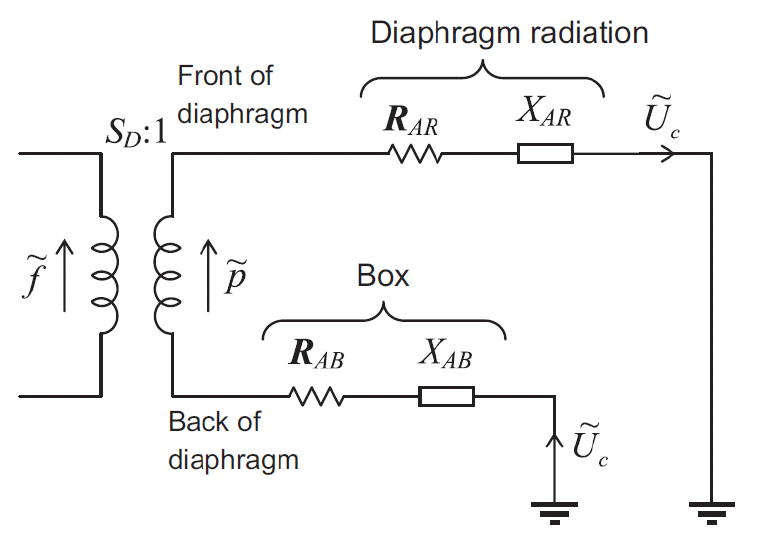
\includegraphics[height=0.16\textheight]{closed_box_circuit_1.png}}
    \hfill
    \subfloat[Complete equivalent circuit]{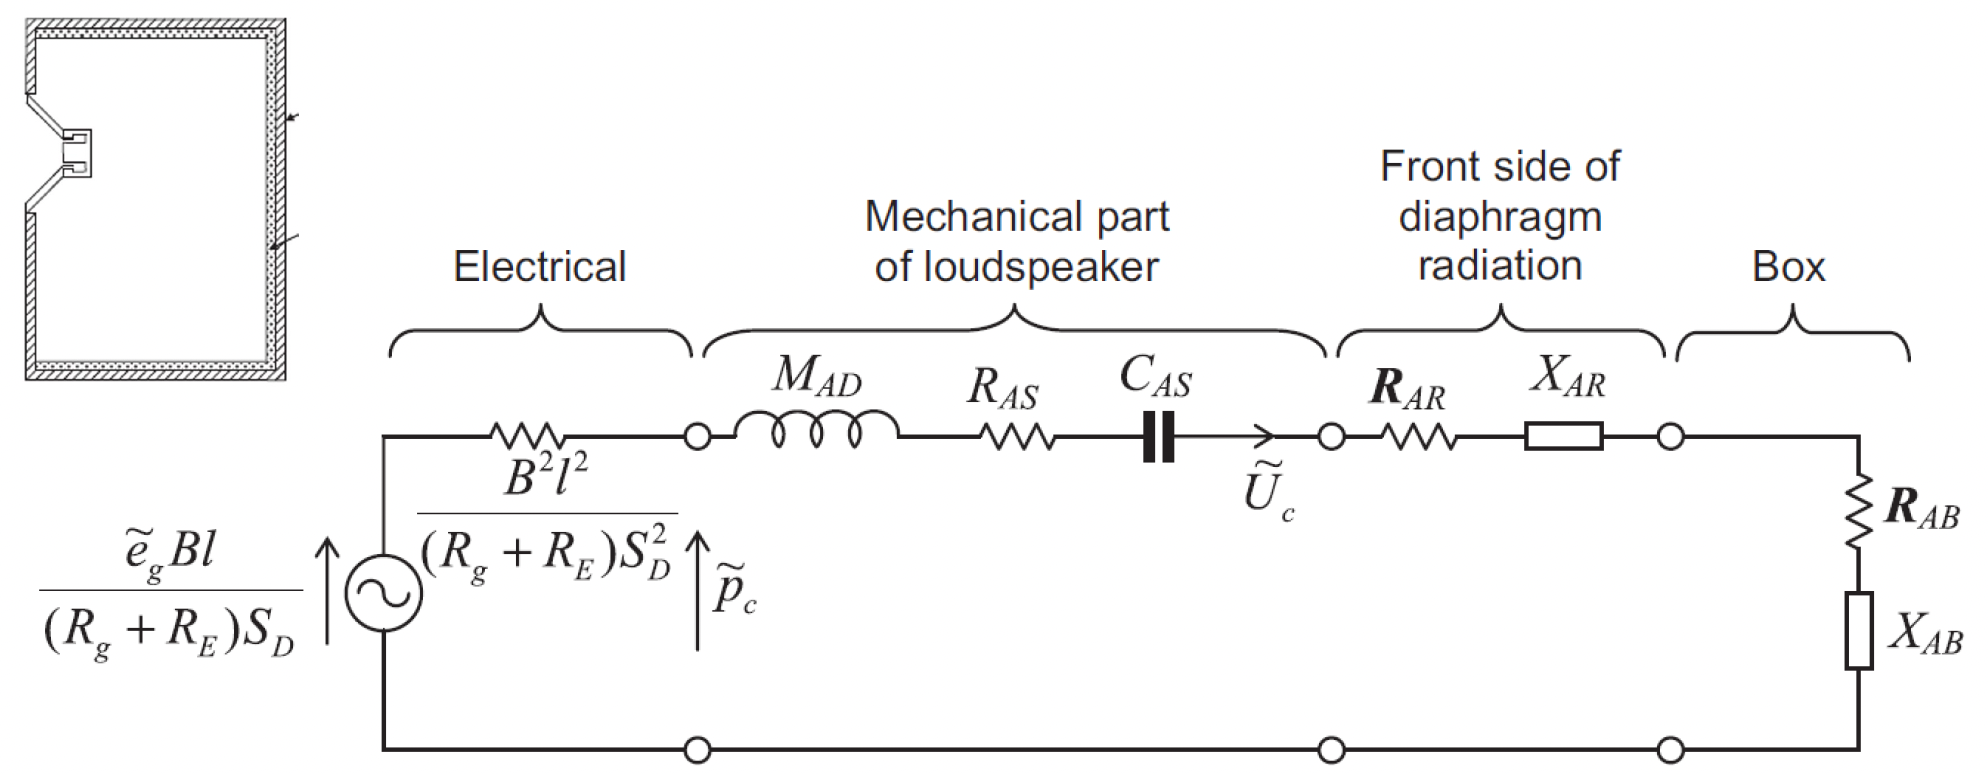
\includegraphics[height=0.16\textheight]{closed_box_circuit.png}}
    \caption{Equivalent circuits for the loudspeaker in a closed-box enclosure. The compliance \(C_{AB}\) of the air in the box appears in parallel with the mechanical suspension compliance \(C_{MS}\), stiffening the total restoring spring}
\end{figure}

\subsection{Closed-Box Resonance Frequency}
\label{ssc:921}

The closed-box resonance frequency \(f_c\) is:
\begin{equation}
    f_c = \frac{1}{2\pi\sqrt{M_{MS} C_{MSB}}}
    \label{eq:fcClosedBox}
\end{equation}
Since the equivalent compliance volume of the suspension is \(V_{AS} = C_{MS} S_D^2 \rho_0 c^2\), and the box compliance volume is \(V_B\), the combined compliance volume is:
\[
\frac{1}{V_{ASB}} = \frac{1}{V_{AS}} + \frac{1}{V_B}
\qquad\Longrightarrow\qquad
V_{ASB} = \frac{V_{AS} V_B}{V_{AS}+V_B}
\]
The ratio of closed-box to free-air resonance frequency is therefore:
\begin{equation}
    \frac{f_c}{f_s} = \sqrt{\frac{C_{MS}}{C_{MSB}}} = \sqrt{1 + \frac{V_{AS}}{V_B}}
    \label{eq:fcRatio}
\end{equation}
Equation \eqref{eq:fcRatio} is the central design relation for closed-box systems.
A box volume equal to \(V_{AS}\) raises the resonance frequency by a factor of \(\sqrt{2}\), approximately half an octave.
A smaller box produces a higher resonance and therefore a reduced bass extension, which is the fundamental trade-off in closed-box design: compactness comes at the cost of low-frequency reach.
In the limiting case of an infinitely large box (\(V_B \to \infty\)), the enclosed air has no effect and \(f_c = f_s\).
In the opposite limit of a very small box (\(V_B \ll V_{AS}\)), the box compliance dominates and the driver resonance is controlled entirely by the air spring: this is the air-suspension (acoustic-suspension) configuration, which trades bass extension for the ability to use a very compliant suspension without risk of overexcursion.

\subsection{Frequency Response and Rolloff}
\label{ssc:922}

The pressure transfer function of a loudspeaker in a closed box is a second-order high-pass filter with the closed-box resonance \(f_c\) and total quality factor \(Q_{TC}\):
\[
\tilde{p}(r) = -\frac{\tilde{e}_g Bl S_D}{(R_g + R_E) M_{MS}} \frac{e^{-jkr}}{4\pi r} \alpha_C(f),
\qquad
\alpha_C(f) = \frac{-(f/f_c)^2}{1 - (f/f_c)^2 + j (f/f_c)/Q_{TC}}
\]
The normalized transfer function \(|\alpha_C(f)|\) is flat well above \(f_c\), peaks at \(f_c\) with a height determined by \(Q_{TC}\), and falls at \(-12 \mathrm{dB/oct}\) below \(f_c\).
This second-order rolloff slope is an intrinsic property of the closed-box topology and cannot be changed without modifying the order of the system.
The total quality factor is:
\[
Q_{TC} = \frac{Q_{EC} Q_{MC}}{Q_{EC} + Q_{MC}}, \qquad Q_{MC} = Q_{MS}\sqrt{1 + \frac{V_{AS}}{V_B}}
\]
The critically damped response (\(Q_{TC} = 1/\sqrt{2} \approx 0.707\)) provides the maximally flat (Butterworth) alignment and is the standard design target for most home-audio closed-box systems.
Values of \(Q_{TC}\) above unity produce a peaked response at \(f_c\) that sounds "boomy" while narrowing the effective bandwidth; values below 0.5 are overdamped and roll off early, giving a thinner bass character.

\begin{figure}[!htb]
    \centering
    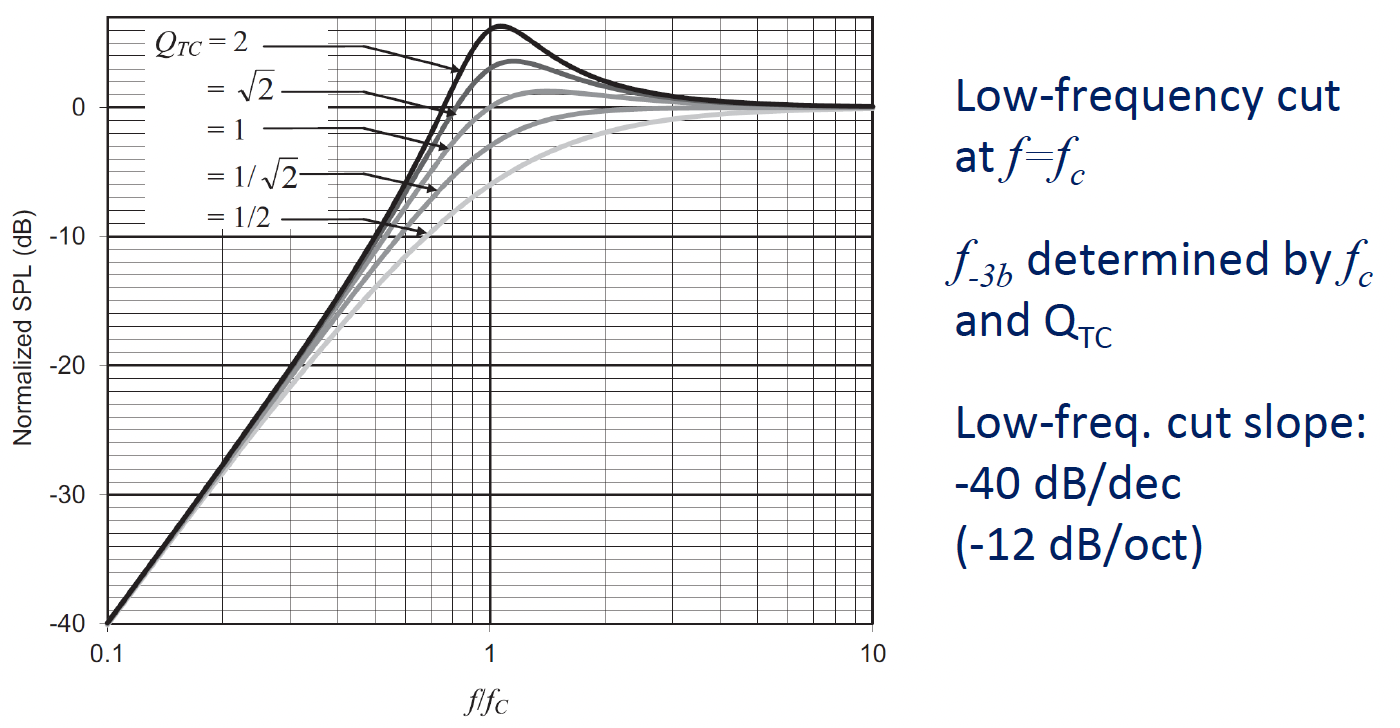
\includegraphics[width=0.55\linewidth]{closed_box_SPL.png}
    \caption{Normalized SPL frequency response of a loudspeaker in a closed-box enclosure for several values of \(Q_{TC}\). The second-order high-pass rolloff of \(-12 \mathrm{dB/oct}\) below \(f_c\) is independent of \(Q_{TC}\); the quality factor determines only the shape of the transition region around \(f_c\)}
\end{figure}

\section{The Bass-Reflex (Vented) Enclosure}
\label{sc:93}

The bass-reflex, or vented-box, enclosure adds an acoustic port to the cabinet: a duct (tube) or slot that connects the interior air volume to the exterior.
The port introduces an additional resonator that can reinforce the bass output below the driver's free-air resonance, extending the usable low-frequency bandwidth compared to a closed-box system of the same volume.
The price paid for this extension is a steeper rolloff below the system cutoff, as will be seen below.

\begin{figure}[!htb]
    \centering
    \subfloat[Schematic model]{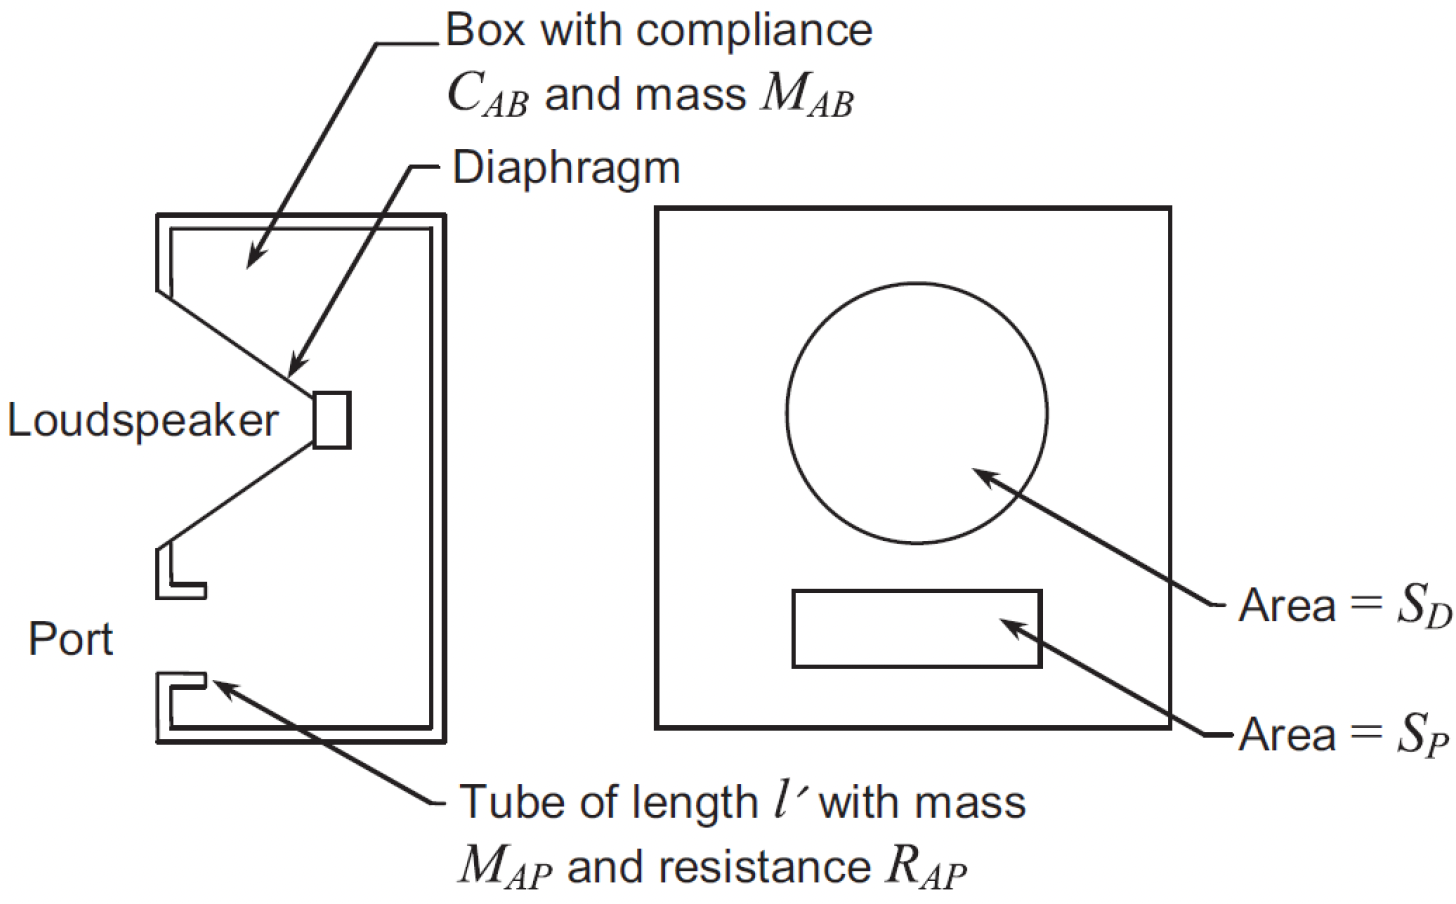
\includegraphics[height=0.22\textheight]{bass_reflex_model.png}}
    \hspace{1cm}
    \subfloat[Air masses and compliances]{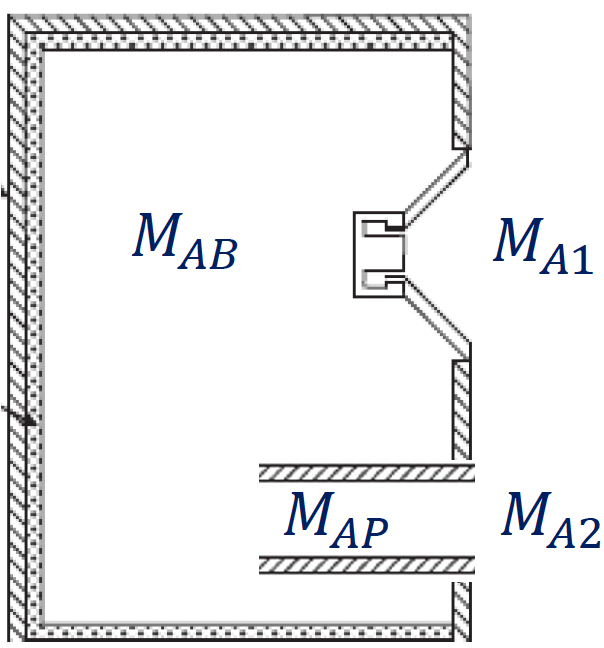
\includegraphics[height=0.22\textheight]{bass_reflex_air_masses.png}}
    \caption{The bass-reflex enclosure. The port duct of cross-section \(S_P\) and length \(t\) provides the acoustic mass \(M_{AT}\); the enclosed air volume \(V_B\) provides the acoustic compliance \(C_{AB}\). Together they form a Helmholtz resonator tuned to the port frequency \(f_B\)}
\end{figure}

\subsection{The Helmholtz Resonator Formed by the Port}
\label{ssc:931}

The air inside a circular port tube of cross-section \(S_P\) and effective length \(t\) (including end corrections) behaves as a lumped acoustic mass:
\[
M_{AT} = \frac{\rho_0 t}{S_P}
\]
The enclosed air volume \(V_B\) provides the acoustic compliance:
\[
C_{AB} = \frac{V_B}{\rho_0 c^2}
\]
Together, \(M_{AT}\) and \(C_{AB}\) form a Helmholtz resonator whose resonance frequency is:
\[
f_B = \frac{1}{2\pi\sqrt{M_{AT} C_{AB}}} = \frac{c}{2\pi}\sqrt{\frac{S_P}{V_B t}}
\]
The port frequency \(f_B\) is the key design parameter of a vented box.
In a typical design it is set close to the driver's free-air resonance \(f_s\), so that the two coupled resonances, one associated with the moving mass \(M_{MS}\) and one with the air mass \(M_{AT}\), produce a flat extended response in the transition band.

\subsection{Behavior at the Port Resonance Frequency}
\label{ssc:932}

The most physically striking property of the bass-reflex system is what happens at \(f_B\): the acoustic impedance of the box-plus-port branch rises to its maximum (the parallel LC resonator is at resonance and presents a very high impedance), so almost no volume velocity flows into the box from the diaphragm.
Instead, the large volume velocity is supplied entirely by the port, which at \(f_B\) oscillates in phase with the front radiation of the driver.
The result is that at the port resonance frequency the diaphragm motion is nearly zero (it is effectively stopped by the back-pressure from the box), while the port radiates the acoustic output.
This is both the strength and the vulnerability of the bass-reflex design: the cone is mechanically unloaded at \(f_B\), so it cannot thermally or mechanically fail, but below \(f_B\) the back-pressure disappears and the cone is free to move with very large excursion, a danger zone for the driver if the signal content extends well below \(f_B\).

\begin{figure}[!htb]
    \centering
    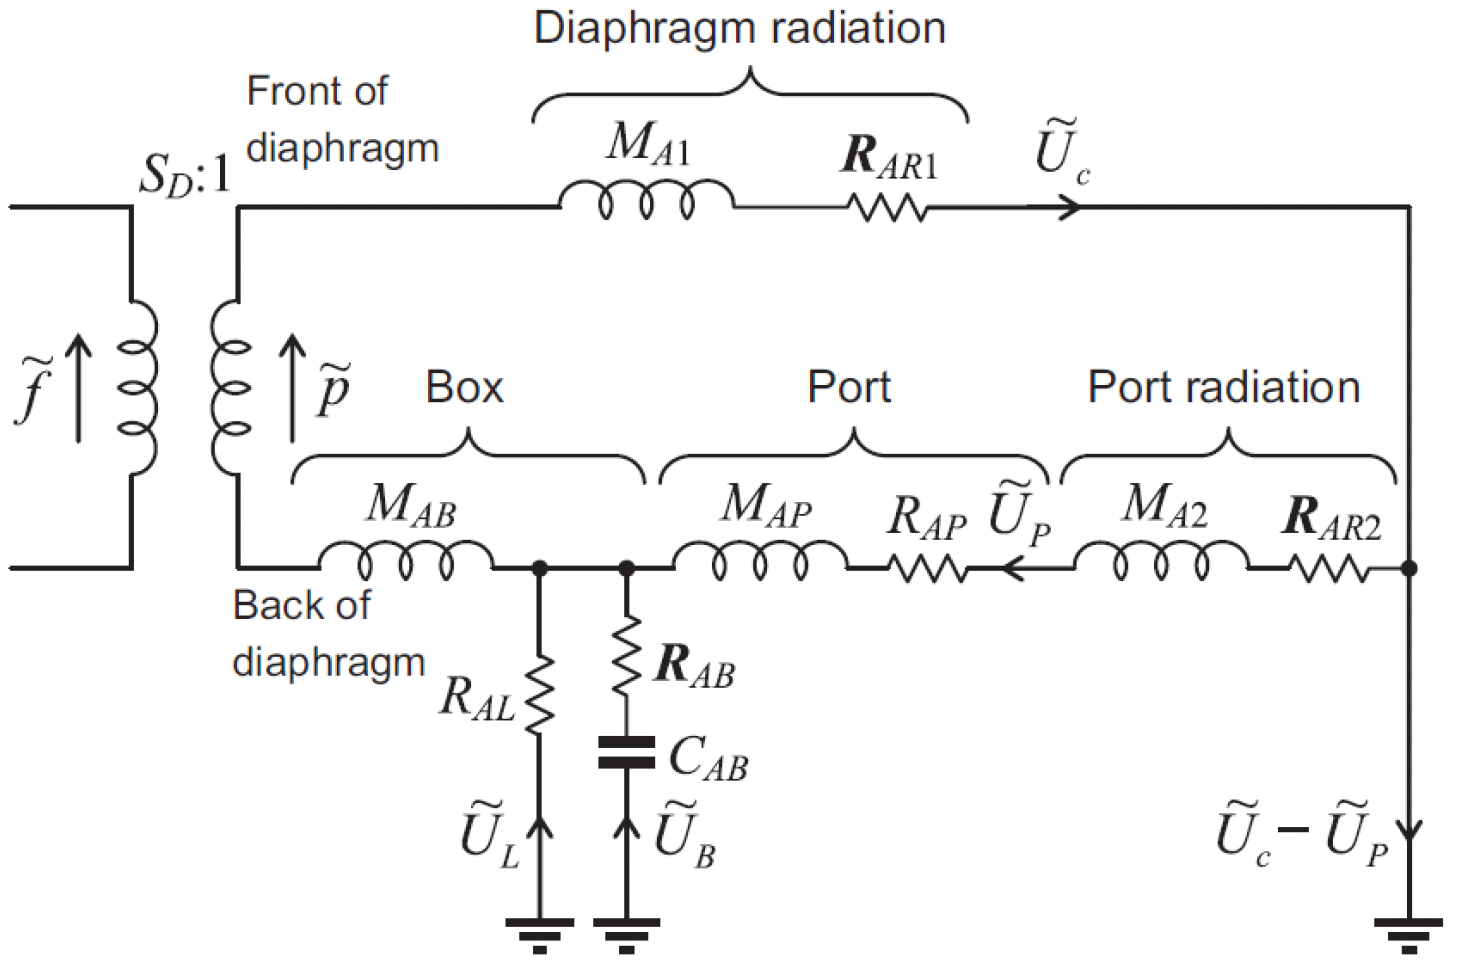
\includegraphics[width=0.70\textwidth]{bass_reflex_circuit.png}
    \caption{Equivalent electro-mechano-acoustic circuit of the bass-reflex loudspeaker. The diaphragm branch (series RLC) and the port branch (parallel LC with compliance \(C_{AB}\) and mass \(M_{AT}\)) are coupled through the box compliance. At \(f_B\) the port branch resonates and presents infinite impedance, stopping the diaphragm and maximizing port output}
\end{figure}

\subsection{Transfer Function and Rolloff Slope}
\label{ssc:933}

The pressure radiated by the combined diaphragm and port is governed by a fourth-order transfer function of the form:
\[
G(s) = \frac{s^4}{s^4 + P_3 s^3 + P_2 s^2 + P_1 s + P_0}
\]
where the coefficients \(P_0\) through \(P_3\) depend on \(\omega_s\), \(\omega_B\), \(Q_{TS}\), and the volume ratio \(V_{AS}/V_B\).
The fourth-order numerator is the defining characteristic of the vented-box topology: it produces a rolloff below the system cutoff of \(-24 \mathrm{dB/oct}\) (or \(-80 \mathrm{dB/dec}\)), steeper by one complete octave-slope than the closed box.
This steeper rolloff protects the driver from infrasonic content above the cutoff but exposes it to large excursions below it, reinforcing the importance of a high-pass filter in the signal chain.

\begin{figure}[!htb]
    \centering
    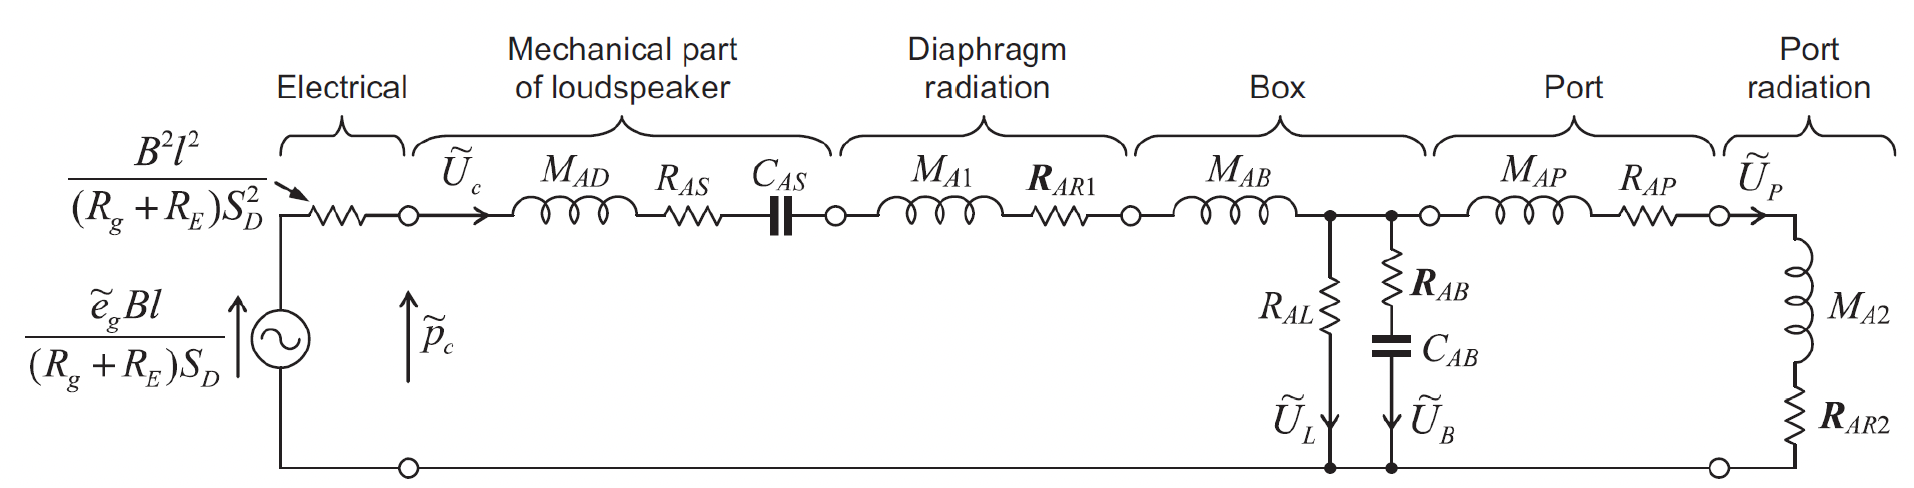
\includegraphics[width=0.90\textwidth]{bass_reflex_complete_scheme.png}
    \caption{Complete schematic representation of the bass-reflex system showing the driver, cabinet, port, and their equivalent-circuit elements. The system has two characteristic frequencies \(\omega_s\) and \(\omega_B\) and a total quality factor \(Q_{TS}\) that together determine the alignment}
\end{figure}

\subsection{Comparison: Closed Box versus Bass-Reflex}
\label{ssc:934}

The two enclosure topologies present a fundamental performance trade-off.
The bass-reflex alignment extends the usable bass response by up to a factor of 1.4 (half an octave) compared to the closed-box alignment for the same driver in the same cabinet volume, because the port resonance adds a second mode that fills in the response below the driver's natural resonance.
On the other hand, the steeper \(-24 \mathrm{dB/oct}\) rolloff below the tuning frequency means that the bass-reflex system is more sensitive to infrasonic transients (thumps, rumble), which can produce very large unloaded cone excursions that exceed the driver's mechanical limits.

\begin{figure}[!htb]
    \centering
    \subfloat[On-axis SPL responses for selected alignments]{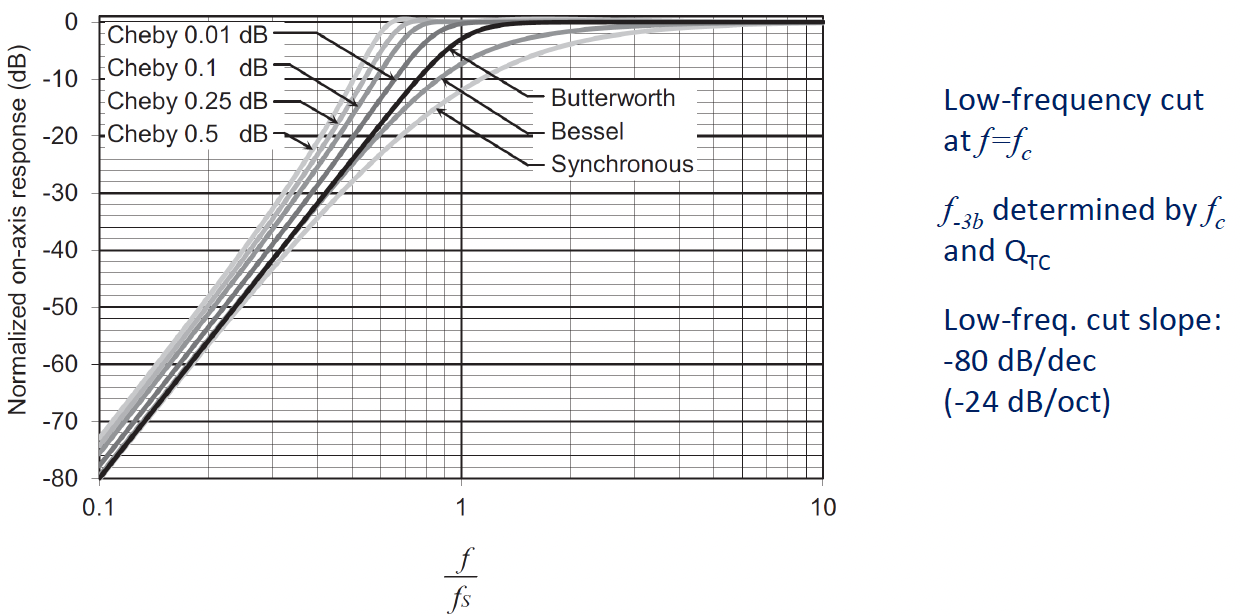
\includegraphics[width=0.46\linewidth]{bass_reflex_SPL.png}}
    \hfill
    \subfloat[Separate contributions of cone and port]{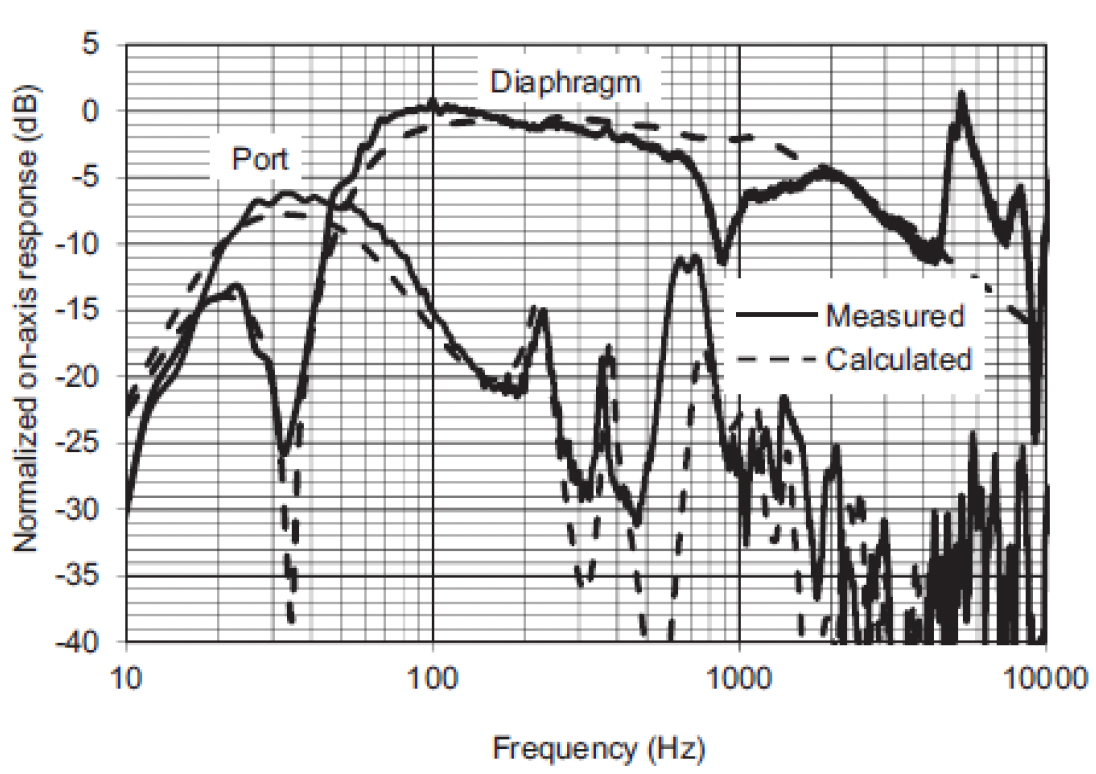
\includegraphics[width=0.46\linewidth]{bass_reflex_SPL_on_axis.png}}
    \caption{Frequency response of the bass-reflex system. The total SPL (left) shows the fourth-order high-pass rolloff of \(-24 \mathrm{dB/oct}\) below the tuning frequency. The individual contributions (right) show that the port dominates the output near \(f_B\) while the driver dominates above and below}
\end{figure}

The selection between the two topologies depends on the application.
Closed-box systems are preferred when group-delay accuracy, resistance to overexcursion, and compact dimensions are paramount.
Bass-reflex systems are preferred when maximum SPL output and extended bass in a given cabinet volume are the primary requirements, and when appropriate crossover filtering can protect the driver below tuning.

    %! TEX root = main.tex

\graphicspath{{00_Images/10_chapter/}}

\chapter{Horn Loudspeakers}
\label{ch:horns}

The direct-radiating loudspeaker analyzed in the preceding chapters suffers from a fundamental inefficiency: the acoustic impedance of air (\(\rho_0 c \approx \SI{407}{\pascal\second\per\meter}\)) is orders of magnitude lower than the mechanical impedance of the vibrating diaphragm-coil assembly, so the coupling between the mechanical source and the acoustic medium is inherently poor.
The horn addresses this mismatch by acting as an acoustic impedance transformer: a continuously flared duct that progressively increases the acoustic pressure while decreasing the particle velocity, converting the high-impedance motion at its narrow throat into a large-area, low-pressure wave at its wide mouth.
The result is a dramatic increase in radiated acoustic power for a given diaphragm velocity, with efficiencies of 10\% to 50\% routinely achieved compared to the sub-2\% typical of direct radiators.

\section{Principle of Operation and Efficiency}
\label{sc:101}

The operating principle of the horn is a direct application of acoustic impedance transformation.
A diaphragm of area \(S_D\) vibrating at velocity \(u_D\) drives a compression driver whose output throat has a much smaller area \(S_T \ll S_D\).
The horn then expands from throat area \(S_T\) to mouth area \(S_M \gg S_T\), so that the acoustic pressure is amplified by the area ratio and the particle velocity is reduced by the same ratio.
Because power is the product of pressure and volume velocity, this redistribution conserves power while improving the match to the radiation impedance of free air.

\paragraph{Why efficiency is so much higher} In a direct-radiating piston, the radiation resistance \(R_s \propto \omega^2\) is much smaller than \(\rho_0 c\) at low frequencies (\(ka \ll 1\)), meaning that most of the mechanical energy stored in the moving mass and spring is never transferred to the air: it simply circulates as reactive energy between the mechanical elements.
The horn eliminates this mismatch by presenting a high acoustic impedance at the throat, which is where the driver delivers its mechanical power.
The driver therefore sees a largely resistive load at all frequencies above the horn's cutoff, and almost all of its mechanical power is converted into radiated sound.
Typical efficiencies for well-designed horn systems range from 10\% to 50\%, compared to less than 2\% for direct-radiating drivers in the same frequency band.
The theoretical work on horn acoustics was established between 1924 and 1928 in two landmark papers: the first appeared in the Journal of the American Institute of Electrical Engineers in 1924, and the second in the Bell System Technical Journal in 1928.
These papers formalized the horn as an acoustic transformer and introduced the exponential and conical horn profiles that remain the most widely used shapes today.

\begin{figure}[!htb]
    \centering
    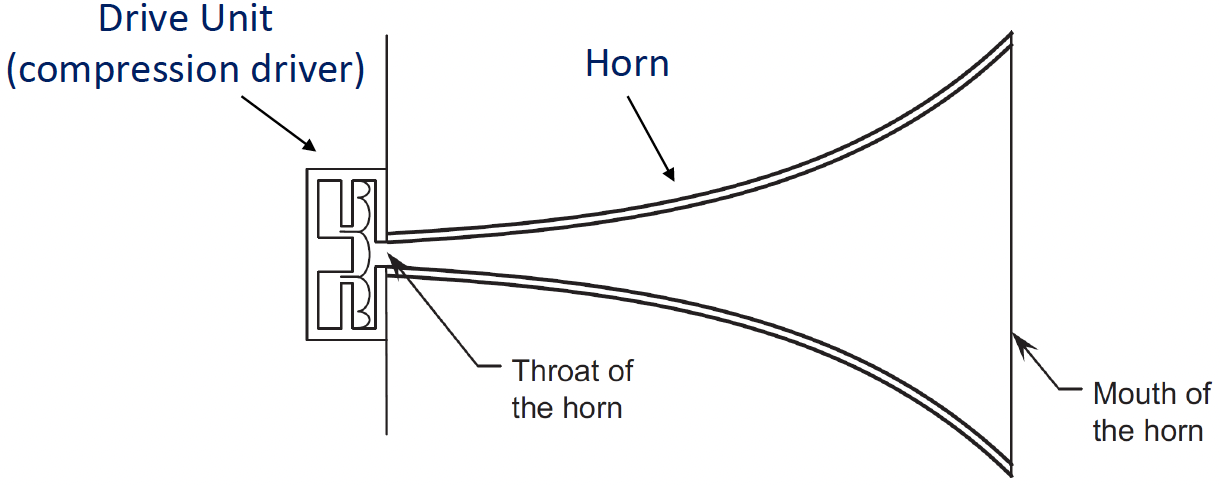
\includegraphics[width=0.70\linewidth]{exp_horn_side.png}
    \caption{Cross-section of a horn loudspeaker with an exponential profile. The compression driver (left) delivers power to the narrow throat of area \(S_T\); the horn expands to the mouth of area \(S_M\), transforming the high-pressure, small-velocity source into a large-area, lower-pressure radiator matched to free air}
    \label{fig:hornSide}
\end{figure}

\section{The Compression Driver}
\label{sc:102}

The transducer element coupled to the horn throat is called a compression driver.
It differs from a conventional direct-radiating driver in both its geometry and its operating impedance.

\subsection{Internal Structure}
\label{ssc:1021}

The compression driver consists of the following elements.
A powerful annular permanent magnet creates a strong radial field in a narrow gap.
A lightweight, rigid diaphragm of area \(S_D\) (typically made from aluminum, titanium, or a composite material) is attached to the voice coil and vibrates axially in response to the Lorentz force.
Behind the diaphragm, a small back cavity provides the acoustic compliance that determines the high-frequency resonance of the driver.
In front of the diaphragm, a phase plug divides the narrow front cavity into multiple radial channels, equalizing the acoustic path length from different parts of the diaphragm to the throat exit.
Without the phase plug, the different path lengths from the diaphragm center and edges to the throat would cause destructive interference at high frequencies, limiting bandwidth.
The throat area \(S_T\) is the cross-section at the exit of the phase plug, where the driver output is delivered to the horn.

\subsection{Throat Mechanical Admittance}
\label{ssc:1022}

The acoustic radiation load seen by the compression driver at the throat of the horn is:
\[
Z_{AT} = \frac{\tilde{P}_T}{\tilde{U}_T} = \rho_0 c S_T
\]
where the last equality assumes that the horn presents a purely resistive plane-wave impedance at its throat.
The corresponding mechanical radiation admittance at the throat, referred through the \(1\colon S_T\) area transformer, is:
\begin{equation}
    Y_{MT} = \frac{1}{\rho_0 c S_T}
    \label{eq:throatAdmittance}
\end{equation}
A smaller throat area \(S_T\) produces a lower mechanical admittance (higher impedance), meaning the driver delivers force more efficiently to the acoustic medium.
This is the design rationale for the compression geometry: by making \(S_T\) much smaller than \(S_D\), the acoustic load seen by the diaphragm is concentrated into a small, high-pressure volume, greatly improving the electromechanical coupling efficiency.

\begin{figure}[!htb]
    \centering
    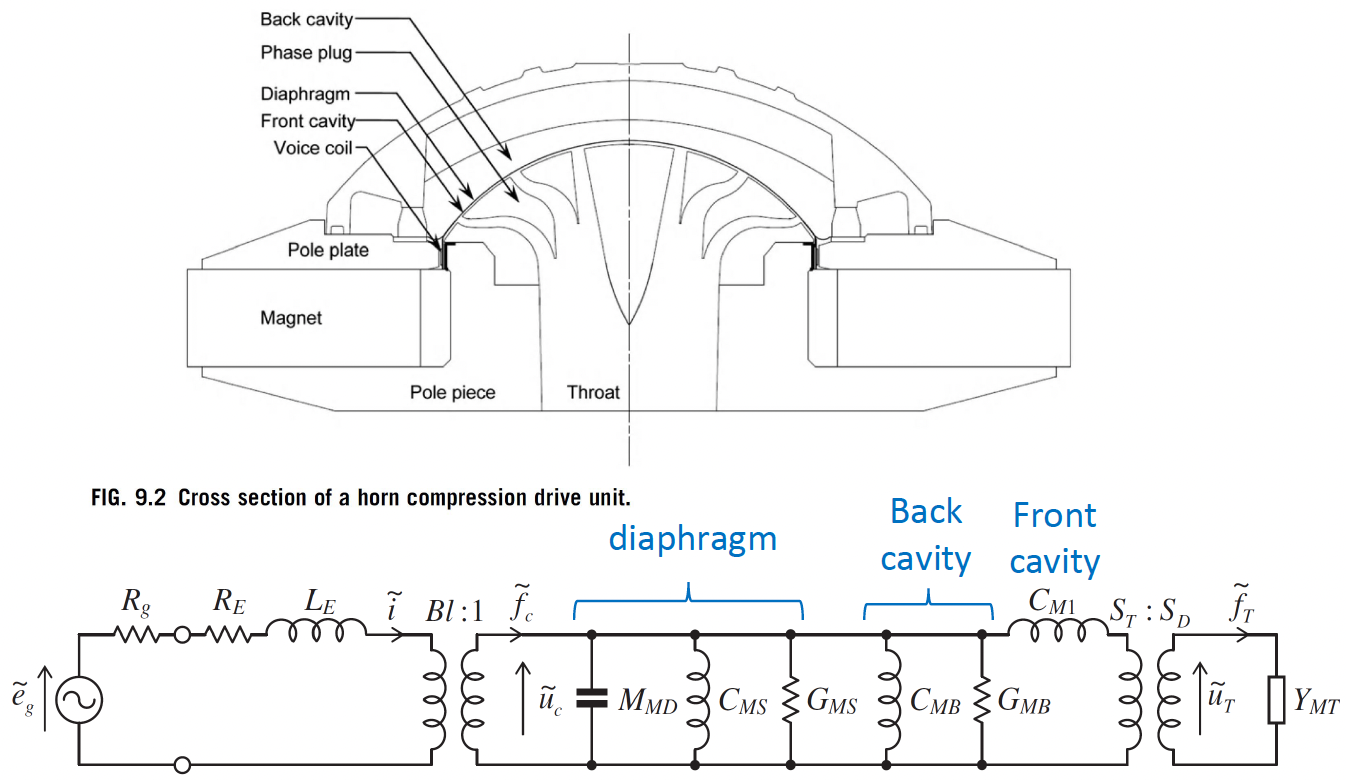
\includegraphics[width=0.90\textwidth]{horn_circuit.png}
    \caption{Electro-mechano-acoustical equivalent circuit of the compression driver and horn (admittance analogy). The driver electrical branch (voice coil \(R_{EC}\), \(L_{EC}\)) drives the mechanical section (diaphragm mass \(M_{MD}\), compliance \(C_{MS}\), damping \(R_{MS}\)) through the transformer of ratio \(Bl\colon 1\). The mechano-acoustic transformer of ratio \(1\colon S_T\) delivers power to the horn throat admittance \(Y_{MT} = 1/(\rho_0 c S_T)\)}
\end{figure}

\section{Horn Profile and Acoustic Gain}
\label{sc:103}

\subsection{Exponential Horn and Cutoff Frequency}
\label{ssc:1031}

The most widely used horn profile is the exponential horn, in which the cross-sectional area expands as:
\[
S(x) = S_T e^{m x}
\]
where \(x\) is the axial coordinate measured from the throat and \(m\) is the flare constant (in \(\si{\per\meter}\)) that controls how rapidly the cross-section expands.
The exponential profile provides the best approximation to a constant-resistance acoustic transmission line: for frequencies above the cutoff frequency, the horn presents a nearly resistive input impedance to the driver.

The cutoff frequency of the exponential horn is:
\begin{equation}
    f_c = \frac{m c}{4\pi}
    \label{eq:hornCutoff}
\end{equation}
Below \(f_c\), the wave equation in the horn has no propagating solutions: acoustic energy is reflected back toward the throat and the horn no longer transmits sound efficiently.
A larger flare constant \(m\) produces a wider-flaring horn with a higher cutoff frequency; a smaller \(m\) produces a narrower horn with a lower cutoff.
Extending the bass response of a horn system requires either a lower \(m\) (gentler flare) or a larger mouth area, both of which increase the physical size of the horn.

\subsection{Alternative Horn Profiles}
\label{ssc:1032}

Several other cross-sectional profiles are used in practice, each offering a different trade-off between bandwidth, directivity, and physical size.

\begin{figure}[!htb]
    \centering
    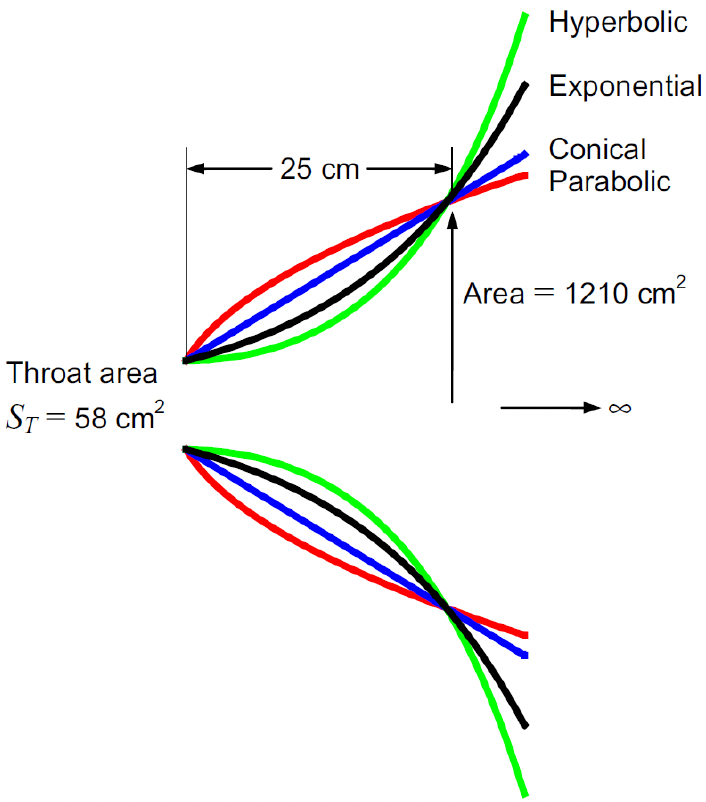
\includegraphics[width=0.60\linewidth]{horn_profiles.png}
    \caption{Cross-sectional profiles of four common horn geometries: exponential, conical, hyperbolic (hypex), and tractrix. The exponential profile provides smooth impedance matching; the tractrix minimizes internal reflections; the conical is simplest to manufacture; the hyperbolic allows independent control of mouth impedance and flare rate}
\end{figure}

The conical horn is the simplest to manufacture and analysis: the area grows as \(S(x) \propto x^2\) from a virtual apex.
It provides good directivity control but less efficient impedance matching than the exponential.
The hyperbolic (or hypex) profile allows the designer to independently control the throat impedance and the expansion rate, making it useful when both low-frequency extension and controlled directivity are required.
The tractrix profile is derived by requiring that wavefronts emerge from the mouth with minimum internal reflection; it is widely used in high-quality studio monitoring horns because its smooth flare minimizes the colorations introduced by reflections inside the horn.

\subsection{Radiation Impedance of the Horn Throat}
\label{ssc:1033}

The normalized throat impedance \(Z_T/(\rho_0 c S_T)\) of a horn depends on both the horn profile and the frequency, and it varies significantly among the different geometries.

\begin{figure}[!htb]
    \centering
    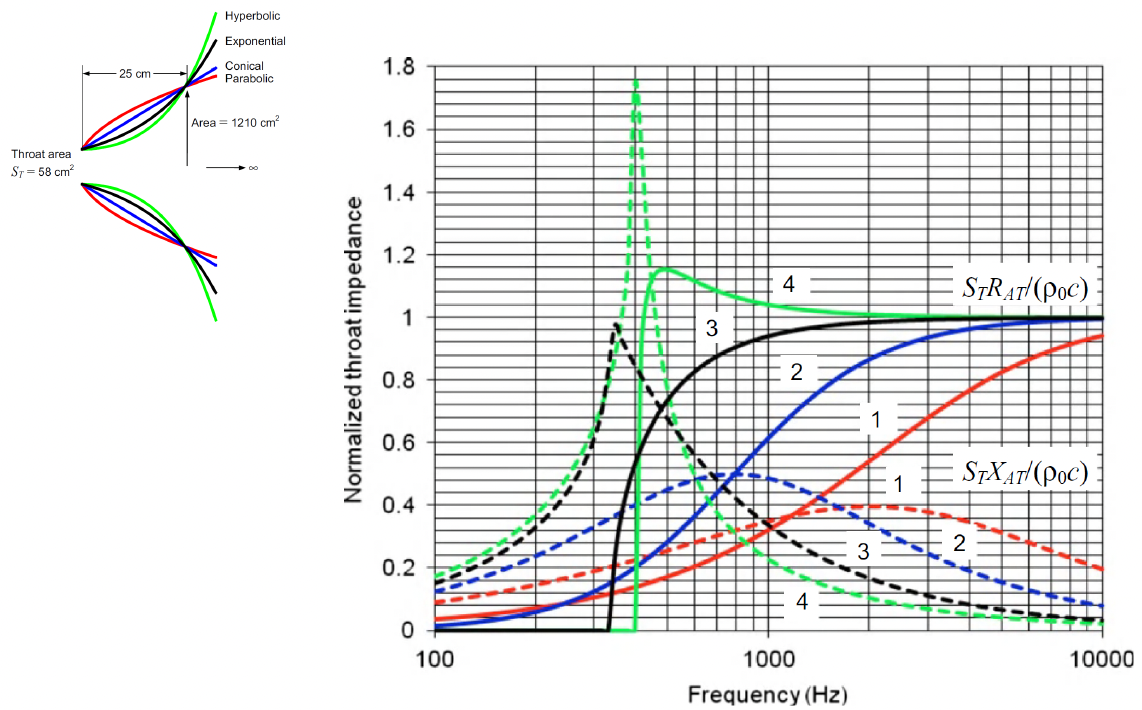
\includegraphics[width=0.65\linewidth]{horn_impedance.png}
    \caption{Normalized throat impedance for four horn profiles: infinite parabolic (1), conical (2), exponential (3), and hyperbolic (4). The resistive part (solid) determines the power transferred to the air; the reactive part (dashed) represents stored energy. Above the cutoff frequency, all profiles approach the plane-wave limit \(\mathrm{Re}[Z]/(\rho_0 c S_T) \to 1\)}
\end{figure}

For the exponential horn above cutoff, the real part of the normalized throat impedance rises steeply from zero at \(f_c\) to unity at high frequencies, confirming that the horn loads the driver with a nearly resistive impedance over its operating band.
Below cutoff, the real part collapses to zero and the throat impedance becomes purely reactive: the driver is loaded by a spring-like or mass-like reactance and no net power is transferred to the air.
This transition from resistive to reactive loading at \(f_c\) is the acoustic analogue of the cutoff of a waveguide, and it sets the hard lower limit of the horn's operating band.

\subsection{Acoustic Gain and Maximum Theoretical Sensitivity}
\label{ssc:1034}

The pressure transformation ratio of the horn from throat to mouth is set by the area ratio \(S_M/S_T\).
In the ideal lossless horn operating above cutoff, the acoustic pressure at the mouth is related to the pressure at the throat by:
\[
\frac{\tilde{P}_T}{\tilde{P}_M} = \sqrt{\frac{S_M}{S_T}}
\]
The maximum theoretical acoustic gain, measured as the ratio of the axial far-field SPL produced by the horn to that of the same driver operating as a direct radiator into free air, is:
\begin{equation}
    G_\mathrm{max} = 20\log_{10}\left(\frac{S_M}{S_T}\right) \quad [\mathrm{dB}]
    \label{eq:hornGain}
\end{equation}
A compression driver with a diaphragm area \(S_D = \pi (5 \mathrm{cm})^2 \approx \SI{78}{\centi\meter\squared}\) coupled through a throat of area \(S_T = \pi (1 \mathrm{cm})^2 \approx \SI{3}{\centi\meter\squared}\) achieves a theoretical gain of \(20\log_{10}(78/3) \approx \SI{28}{\decibel}\).
In practice, internal reflections, diffraction losses at the mouth, and non-ideal wavefront geometry reduce this by 5 dB to 10 dB, but even the achievable gain of 15 dB to 25 dB represents an enormous improvement in sensitivity compared to direct-radiating designs.

\subsection{Directivity and Bandwidth}
\label{ssc:1035}

The far-field directivity of a horn loudspeaker is controlled by the mouth geometry.
At low frequencies (mouth circumference much smaller than the wavelength), the radiation is nearly omnidirectional.
As frequency rises and the mouth dimensions become comparable to the wavelength, the radiation narrows into an increasingly sharp beam along the horn axis, following the same physics as the piston directivity analyzed in chapter \ref{ch:sound_radiation}.
The cutoff frequency at which the mouth starts to beam is:
\[
f_0 = \frac{c}{2\pi a_M}
\]
where \(a_M = \sqrt{S_M/\pi}\) is the equivalent radius of the mouth.
The table in chapter \ref{ch:sound_radiation} (section \ref{sc:62}) gives representative values: a mouth of radius \SI{30}{\centi\meter} has \(f_0 \approx \SI{183}{\hertz}\), so the horn is effectively omnidirectional below that frequency and progressively more directional above it.
Constant-directivity (CD) horn designs address the high-frequency beaming problem by modifying the flare shape near the throat to introduce controlled diffraction, maintaining a uniform coverage angle across the operating band at the cost of some efficiency.
These designs are standard in professional sound reinforcement, where consistent audience coverage is more important than maximum on-axis sensitivity.

\begin{figure}[!htb]
    \centering
    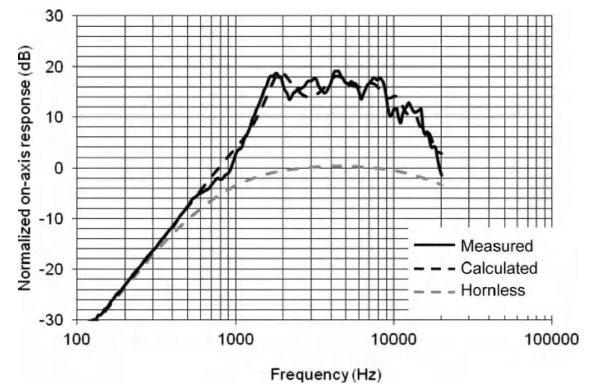
\includegraphics[width=0.55\linewidth]{horn_directivity.png}
    \caption{On-axis SPL frequency response of a high-frequency horn driver (solid curve). The flat response region extends from approximately \SI{1}{\kilo\hertz} to \SI{20}{\kilo\hertz}, corresponding to the band in which the horn presents a resistive throat impedance and the driver diaphragm operates in its mass-controlled regime}
\end{figure}

    %! TEX root = main.tex

\graphicspath{{00_Images/11_chapter/}}

\chapter{Introduction to Microphones and Specifications}
\label{ch:microphone_intro}

A microphone is an electroacoustic transducer that converts acoustic pressure variations in the surrounding sound field into a corresponding electrical voltage at its output terminals.
In this sense it performs the inverse function of the electrodynamic loudspeaker studied in the preceding chapters: rather than driving a diaphragm to radiate sound, the microphone senses the mechanical displacement imposed on a diaphragm by an incoming wave and delivers an electrical signal proportional to the sound pressure.
Microphones are classified along three independent axes.
According to the transduction principle, the main families are condenser (capacitor), moving-coil (dynamic) and piezoelectric (crystal) types.
According to function, a microphone may be designed for calibrated sound-level measurement, for speech or sound reinforcement or for studio and recording applications.
According to directional characteristic, the sensitivity pattern can be omnidirectional, cardioid, supercardioid or hypercardioid, depending on how the capsule is exposed to the sound field.
This chapter presents the principal transduction mechanisms, defines the key performance parameters, sensitivity, noise, dynamic range and frequency response and provides an overview of directional behavior that will be developed quantitatively in the chapters that follow.

\section{Transduction Principles}
\label{sc:111}

The history of the microphone spans roughly a century of progressive refinement, beginning with electrochemical and electromagnetic techniques and culminating in the precision capacitive transducers that dominate modern studio and measurement practice.
The following survey introduces each mechanism at the level of detail needed to understand why condenser and moving-coil types have displaced the earlier designs and how the underlying physics shapes the practical characteristics of each family.

\subsection{Historical Types}

\paragraph{Carbon microphone} The carbon microphone, introduced commercially by Westinghouse around 1921, operates on a piezoresistive principle.
A metallic diaphragm is pressed against a cup filled with carbon granules; acoustic pressure deforms the diaphragm, compressing or expanding the granule bed and thereby changing the electrical resistance of the medium.
A DC voltage applied across the element converts this resistance variation into a current signal, which is then stepped up in voltage by a series transformer that simultaneously performs AC coupling and impedance transformation to the load.
Despite its historical importance as the dominant telephone transducer for several decades, the carbon microphone suffers from high self-noise, strong nonlinear distortion and a frequency response that rolls off markedly above a few kilohertz and it has been completely superseded in all audio applications.

\paragraph{Ribbon microphone} The ribbon microphone, developed around 1933, suspends a thin corrugated metallic ribbon in the gap of a permanent magnet.
Incident sound waves set the ribbon into velocity-proportional vibration and, by Faraday's induction law, a voltage proportional to the ribbon velocity is induced along its length.
Because the ribbon element is intrinsically a low-impedance, low-voltage source, a step-up transformer is mounted directly behind it to deliver a usable signal level to the preamplifier.
The ribbon microphone exhibits a natural figure-eight (bidirectional) polar pattern, an extended and smooth frequency response and a characteristic warm tonal quality valued for orchestral and vocal recording; its practical limitations are mechanical fragility and sensitivity lower than that of condenser types.

\paragraph{Crystal microphone} The crystal or piezoelectric, microphone relies on the direct piezoelectric effect: mechanical deformation of a crystalline material generates an electric charge across its faces.
Sound waves displace a lightweight diaphragm that presses against a piezoelectric element, producing an output voltage proportional to the applied pressure.
Crystal microphones are mechanically simple and inexpensive, but they exhibit high output impedance, limited frequency range and poor environmental stability, making them unsuitable for professional applications.

\subsection{Moving-Coil Microphone}

The moving-coil microphone, also called the dynamic microphone, operates on the same electromagnetic principle as the electrodynamic loudspeaker, but with the direction of energy conversion reversed.
A lightweight diaphragm, typically fabricated from a polyester film such as Mylar, is mechanically coupled to a cylindrical coil of fine wire wound around a former that sits in the annular gap of a permanent magnet.
Incident acoustic pressure displaces the diaphragm, which carries the coil axially through the static magnetic field; by the Lorentz law applied in reverse, this motion induces an electromotive force across the coil terminals proportional to the coil velocity:
\[
v_{\mathrm{out}} = B l u_c
\]
where \(B\) is the magnetic flux density in the gap, \(l\) is the total effective length of wire immersed in the field and \(u_c\) is the instantaneous coil velocity.
Because the moving-coil capsule is sensitive to external low-frequency magnetic interference such as that produced by power-line transformers, a compensating hum-bucking coil wound in opposition is commonly incorporated to cancel the induced interference.
Moving-coil microphones require no polarization voltage, tolerate high sound pressure levels without distortion and are mechanically robust against rough handling and adverse environmental conditions, making them the standard choice for live sound reinforcement and broadcast applications.

\subsection{Condenser Microphone}

The condenser (capacitor) microphone represents the most accurate and most widely used transduction principle in both professional recording and precision measurement.
Its capsule consists of two electrically conductive elements separated by a narrow air gap of approximately \SIrange{15}{30}{\micro\meter}: a thin, tensioned metallic diaphragm exposed to the sound field and a fixed, perforated backplate.
Together they form a capacitor with capacitance:
\[
C = \varepsilon \frac{A}{d}
\]
where \(\varepsilon\) is the permittivity of air, \(A\) is the effective electrode area and \(d\) is the gap distance.

\begin{figure}[!htb]
    \centering
    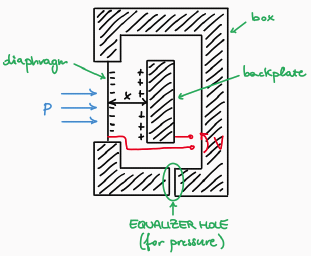
\includegraphics[width=0.45\textwidth]{condenser_mic.png}
    \caption{Cross-section of a condenser microphone capsule showing the tensioned diaphragm, the \SIrange{15}{30}{\micro\meter} air gap and the perforated backplate}
\end{figure}

The capsule is held at a constant charge \(Q\) by a high-impedance DC bias circuit, so that the capacitor law \(Q = C V\) implies:
\[
\Delta V \approx -V_B \frac{\Delta C}{C_0} \approx V_B \frac{\Delta d}{d_0}
\]
where \(V_B\) is the bias voltage, \(C_0\) is the equilibrium capacitance and \(d_0\) is the equilibrium gap.
The output voltage is therefore directly proportional to the diaphragm displacement and since that displacement is proportional to acoustic pressure in the stiffness-controlled regime, the transduction chain is linear: \(v_{\mathrm{out}} \propto p\).
A standard bias of \SI{48}{\volt} (phantom power) is supplied symmetrically through the balanced XLR cable and used to polarize the capsule and power the internal impedance-converter circuitry.
The condenser principle offers lower noise, wider frequency range and higher sensitivity than all other transduction types; its only practical requirements are a stable bias supply and careful management of humidity, since the very high bias impedance renders the capsule susceptible to surface contamination.

\section{Sensitivity and Sound Pressure Level}
\label{sc:112}

\subsection{Sensitivity Definition}

The sensitivity \(S\) of a microphone is the fundamental figure of merit that quantifies how efficiently acoustic pressure is converted into an electrical voltage at the output terminals.
It is defined as the ratio of the open-circuit output voltage \(v_{\mathrm{out}}\) to the incident sound pressure \(p\), measured at a specified reference frequency (conventionally \SI{1}{\kilo\hertz}) under free-field conditions with the wave arriving on-axis:
\[
S = \frac{v_{\mathrm{out}}}{p} \quad \left[\si{\volt\per\pascal}\right]
\]
A typical value for a professional condenser microphone is \(S = \SI{10}{\milli\volt\per\pascal}\).
Because the sensitivity spans many orders of magnitude across different microphone classes, it is more conveniently expressed in decibels relative to the standard reference value \(S_{\mathrm{REF}} = \SI{1}{\volt\per\pascal}\):
\[
S_{\mathrm{dB}} = 20\log_{10}\left(\frac{S}{S_{\mathrm{REF}}}\right)
\]
Some representative values and their decibel equivalents are listed below:
\begin{itemize}
    \item \SI{1}{\volt\per\pascal} \(\to\) \(\SI{0}{\decibel} \mathrm{V/Pa}\)
    \item \SI{100}{\milli\volt\per\pascal} \(\to\) \(-20 \mathrm{dB} \mathrm{V/Pa}\)
    \item \SI{10}{\milli\volt\per\pascal} \(\to\) \(-40 \mathrm{dB} \mathrm{V/Pa}\)
    \item \SI{1}{\milli\volt\per\pascal} \(\to\) \(-60 \mathrm{dB} \mathrm{V/Pa}\)
    \item \SI{100}{\micro\volt\per\pascal} \(\to\) \(-80 \mathrm{dB} \mathrm{V/Pa}\)
\end{itemize}

\subsection{Sound Pressure Level}

The sound pressure level (SPL) is defined as:
\[
\mathrm{SPL} = 20\log_{10}\left(\frac{p_{\mathrm{RMS}}}{p_{\mathrm{ref}}}\right) \quad [\mathrm{dB SPL}]
\]
where the reference pressure \(p_{\mathrm{ref}} = \SI{20}{\micro\pascal}\) corresponds to the threshold of hearing at \SI{1}{\kilo\hertz} for a young person with normal hearing and defines the \SI{0}{\decibel} point of the SPL scale.
The acoustic domain of interest for audio applications spans from \SI{0}{\decibel SPL} (threshold of audibility, \(\approx \SI{20}{\micro\pascal}\)) to approximately \SI{140}{\decibel SPL} (threshold of pain, \(\approx \SI{200}{\pascal}\)), covering seven decades of absolute pressure.
Since the microphone output voltage is proportional to pressure through the sensitivity, any position on the SPL axis maps directly to a corresponding output voltage: for \(S = \SI{10}{\milli\volt\per\pascal}\), a conversation at \SI{60}{\decibel SPL} produces roughly \SI{20}{\milli\pascal} and thus \(\SI{0.2}{\milli\volt}\) at the microphone output, while a nearby jackhammer at \SI{100}{\decibel SPL} produces \SI{2}{\pascal} and \SI{20}{\milli\volt}.

\subsection{Specification Example: Shure KSM9}

The Shure KSM9 electret condenser microphone illustrates how the sensitivity specification is applied in practice.
Its data sheet lists:
\begin{itemize}
    \item Sensitivity (open-circuit, at \SI{1}{\kilo\hertz}): \(-51 \mathrm{dBV/Pa}\), equivalent to \(\SI{2.8}{\milli\volt\per\pascal}\)
    \item Maximum SPL at \SI{1}{\percent} THD: \SI{152}{\decibel SPL}
    \item Self-noise: \SI{22}{\decibel SPL} (A-weighted)
    \item Dynamic range: \SI{130}{\decibel}
\end{itemize}
The maximum SPL corresponds to an acoustic pressure of:
\[
p_{\mathrm{max}} = \SI{20}{\micro\pascal} \times 10^{152/20} \approx \SI{796}{\pascal}
\]
yielding a peak output voltage of:
\[
v_{\mathrm{out,max}} = S \times p_{\mathrm{max}} = \SI{2.8}{\milli\volt\per\pascal} \times \SI{796}{\pascal} \approx \SI{2.2}{\volt}
\]
This figure sets the clipping level that the preamplifier input stage must accommodate without distortion.
Conversely, at a quiet conversational SPL of \SI{60}{\decibel SPL} the output is only \SI{0.06}{\milli\volt}, illustrating the enormous dynamic range the downstream electronics must handle, from microvolts to volts within the same system.

\section{Directionality}
\label{sc:113}

\subsection{Directional Sensitivity}

The sensitivity of a microphone depends in general on the direction from which the sound arrives.
This angular dependence is characterized by the relative directional sensitivity function:
\[
S_{\mathrm{REL}}(\alpha) = \frac{S(\alpha)}{S(0)}
\]
where \(\alpha\) is the angle of incidence measured from the diaphragm normal axis and \(S(0)\) is the on-axis sensitivity.
Expressed in decibels:
\[
S_{\mathrm{REL},\mathrm{dB}}(\alpha) = 20\log_{10}\left(\frac{S(\alpha)}{S(0)}\right)
\]
Since the on-axis direction \(\alpha = 0\) typically corresponds to maximum sensitivity, \(S_{\mathrm{REL}}(\alpha) \leq 1\) and \(S_{\mathrm{REL},\mathrm{dB}}(\alpha) \leq 0 \mathrm{dB}\) for all other angles.
The complete angular dependence is displayed as a polar pattern, which plots \(S_{\mathrm{REL},\mathrm{dB}}(\alpha)\) in polar coordinates on concentric reference circles conventionally spaced at \SI{5}{\decibel} or \SI{10}{\decibel} intervals.

\subsection{Polar Pattern Types}

The principal directional characteristics encountered in practice are shown in figure \ref{fig:polarPatterns}.

\begin{figure}[!htb]
    \centering
    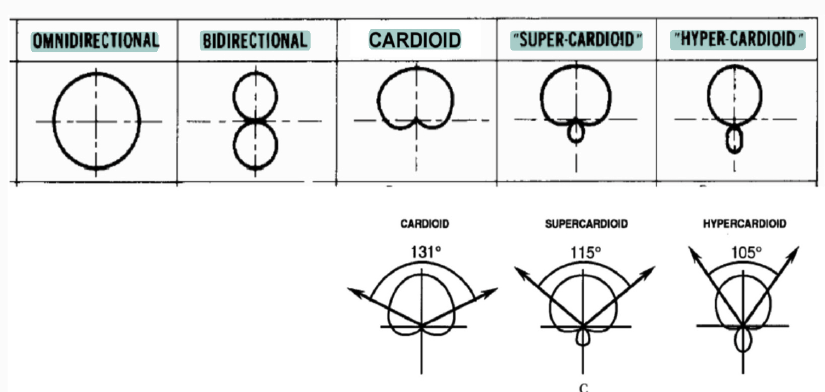
\includegraphics[width=0.80\textwidth]{directivity_pattern.png}
    \caption{Principal microphone polar patterns: omnidirectional, cardioid, supercardioid, hypercardioid and bidirectional (figure-eight)}
    \label{fig:polarPatterns}
\end{figure}

An omnidirectional microphone responds equally to sound from all directions (\(S_{\mathrm{REL}}(\alpha) = 1\) for all \(\alpha\)), while a bidirectional (figure-eight) microphone responds equally from the front and rear but exhibits a null at the sides (\(\alpha = 90°\)).
Intermediate patterns, obtained by combining pressure and pressure-gradient sensing as analyzed in the following chapter, yield the cardioid, supercardioid and hypercardioid families.
The cardioid exhibits a null at \(\alpha = 180°\), while the supercardioid and hypercardioid achieve a narrower main lobe at the expense of a small rear lobe.
Because of their forward-oriented pickup, directional microphones offer a higher ratio of on-axis to ambient response than the omnidirectional pattern: at equal working distance, a cardioid rejects diffuse ambient sound approximately \SI{4.8}{\decibel} more effectively than an omnidirectional microphone, a supercardioid provides \SI{5.8}{\decibel} more rejection and a hypercardioid provides \SI{6}{\decibel} more.
Equivalently, a cardioid may be placed approximately \(1.7\) times farther from the source than an omnidirectional microphone while maintaining the same signal-to-ambient ratio, a supercardioid at \(1.9\) times and a hypercardioid at \(2\) times.

\subsection{Omnidirectional Microphones}

Omnidirectionality is achieved by exposing the diaphragm to the sound field exclusively through a single front entry, so that the rear of the diaphragm is enclosed in a sealed cavity at ambient pressure.
At low frequencies, where the acoustic wavelength \(\lambda\) greatly exceeds the microphone body diameter \(D\), diffraction wraps the wave around the body and the capsule acts as a point obstacle: the pressure field reaches the diaphragm with essentially the same amplitude regardless of the direction of incidence and the response is genuinely omnidirectional.
At high frequencies, when \(\lambda\) becomes comparable to \(D\), the microphone body casts an acoustic shadow on the rear face of the capsule and the response becomes strongly direction-dependent.
The condition for omnidirectional behavior at a given frequency is therefore:
\[
\lambda > 10 D \quad \Longrightarrow \quad f < \frac{c}{10 D} \approx \frac{3}{D [\mathrm{cm}]} \mathrm{kHz}
\]
A capsule intended to remain omnidirectional up to \SI{20}{\kilo\hertz} must have a diaphragm diameter no larger than approximately \SI{1.7}{\milli\meter}; a standard half-inch (\SI{12.7}{\milli\meter}) capsule begins to exhibit directional narrowing above roughly \SI{2.4}{\kilo\hertz}.

\begin{figure}[!htb]
    \centering
    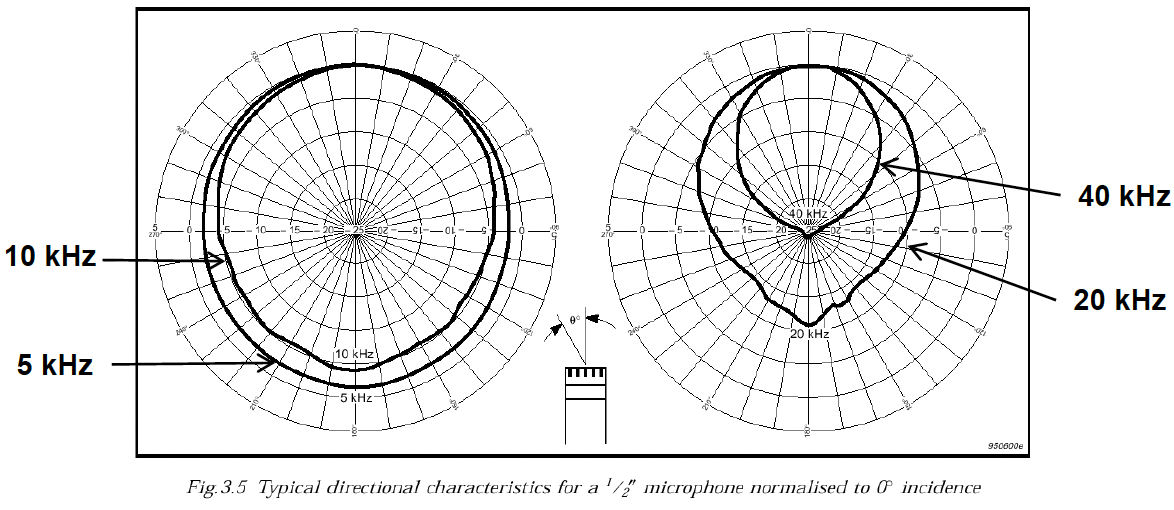
\includegraphics[width=0.70\textwidth]{omni_mic.png}
    \caption{Directional characteristics of a \(\tfrac{1}{2}''\) omnidirectional microphone normalized to \(0°\) incidence, showing the progressive departure from omnidirectionality as frequency increases from \SI{5}{\kilo\hertz} to \SI{40}{\kilo\hertz}: the acoustic shadow effect confines the effective pickup angle as \(\lambda\) approaches \(D\)}
\end{figure}

\subsection{Directional Microphones}

Directional microphones achieve their pattern by providing acoustic access to both the front and the rear of the diaphragm through multiple entries.
The rear entry is connected to the diaphragm through an internal acoustic path that introduces a delay of approximately one half-period at the design frequency, so that the rear wave arrives out of phase with the front wave.
For sound arriving from the front (\(\alpha = 0°\)), the front wave and the phase-shifted rear wave reinforce each other in displacing the diaphragm, producing maximum sensitivity.
For sound arriving from the rear (\(\alpha = 180°\)), both sides of the diaphragm receive the same wave simultaneously, so the two contributions cancel and the net diaphragm displacement is zero.

\begin{figure}[!htb]
    \centering
    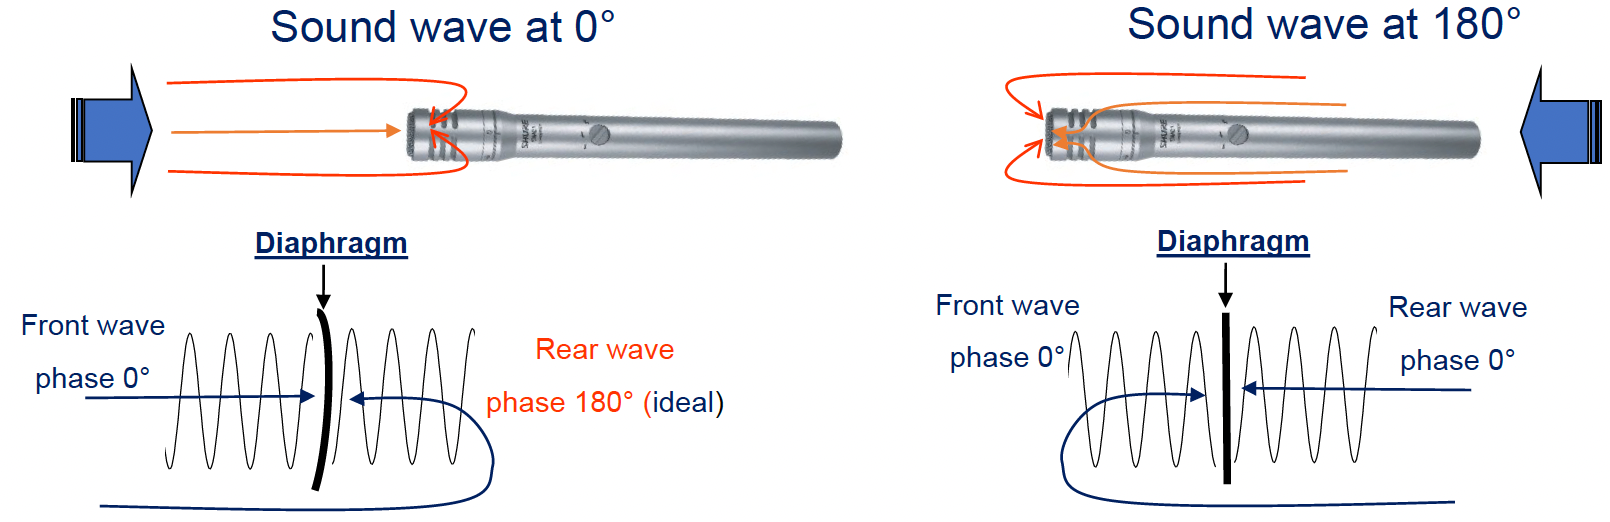
\includegraphics[width=0.80\textwidth]{directional_mic.png}
    \caption{Operating principle of a directional microphone with front and rear acoustic entries: a wave arriving at \(0°\) drives the diaphragm coherently through the delayed rear path (left), while a wave arriving at \(180°\) reaches both faces simultaneously and produces cancellation (right)}
\end{figure}

Some high-performance condenser microphones incorporate two diaphragms oriented in opposite directions and sharing a common backplate.
By varying the relative bias voltages applied to the two capsule halves, the polar pattern is adjusted continuously from omnidirectional through wide-angle cardioid, cardioid, hypercardioid and bidirectional, without any mechanical modification of the capsule.
The directionality in a real acoustic environment may differ substantially from the free-field polar pattern: nearby reflecting surfaces, including a human head positioned close to the microphone, scatter and redirect sound so that energy nominally arriving from the rear reaches the diaphragm from other directions, partially reducing the intended rear rejection.

\begin{figure}[!htb]
    \centering
    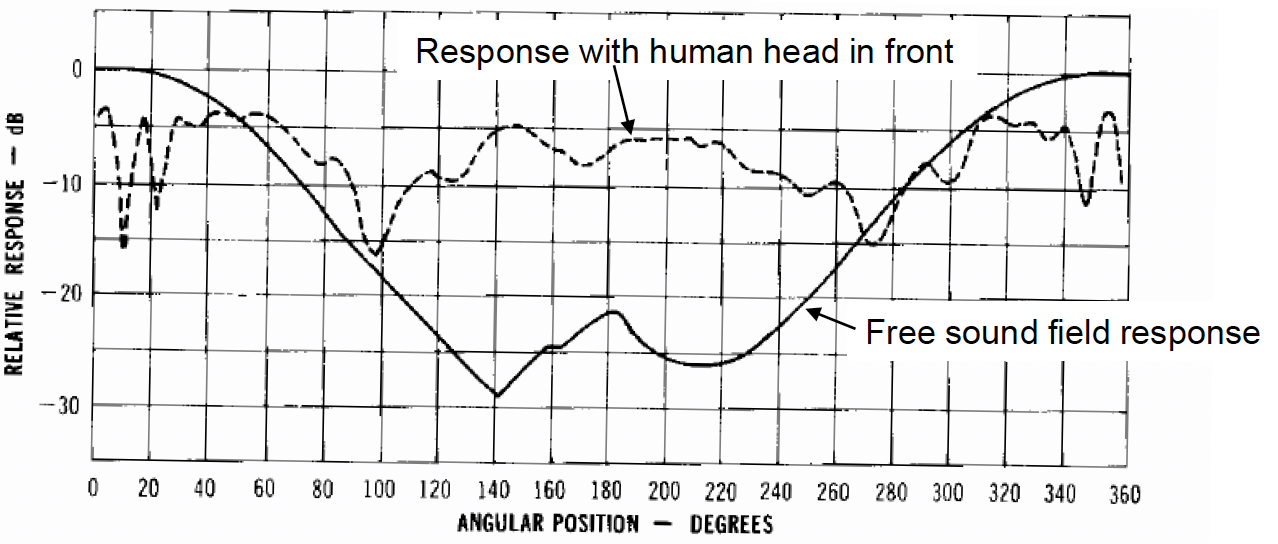
\includegraphics[width=0.70\textwidth]{obstacle_consequence.png}
    \caption{Effect of a nearby head obstacle on the effective polar response of a cardioid microphone: mid-frequency reflections off the head partially fill the rear null, illustrated by the dashed curve compared to the free-field response (solid curve)}
\end{figure}

\subsection{Highly Directional Microphones}

When the working distance between source and microphone is large, the sound pressure at the capsule drops significantly, requiring increased preamplifier gain, which simultaneously raises the captured level of diffuse ambient noise.
Interference-tube microphones (commonly called shotgun microphones) address this problem by placing a long tube of \SIrange{20}{40}{\centi\meter} with multiple lateral apertures in front of a directional capsule.
Off-axis sound waves enter the tube at multiple apertures spaced along its length and travel different distances to the diaphragm, accumulating phase shifts that produce destructive interference; on-axis sound waves travel directly to the far end of the tube and are captured coherently.
The resulting polar pattern is considerably narrower than a standard cardioid, enabling precise aiming at a distant source with strong rejection of off-axis and ambient contributions.

\begin{figure}[!htb]
    \centering
    \subfloat[Polar pattern of the Sennheiser MKH416 shotgun microphone]{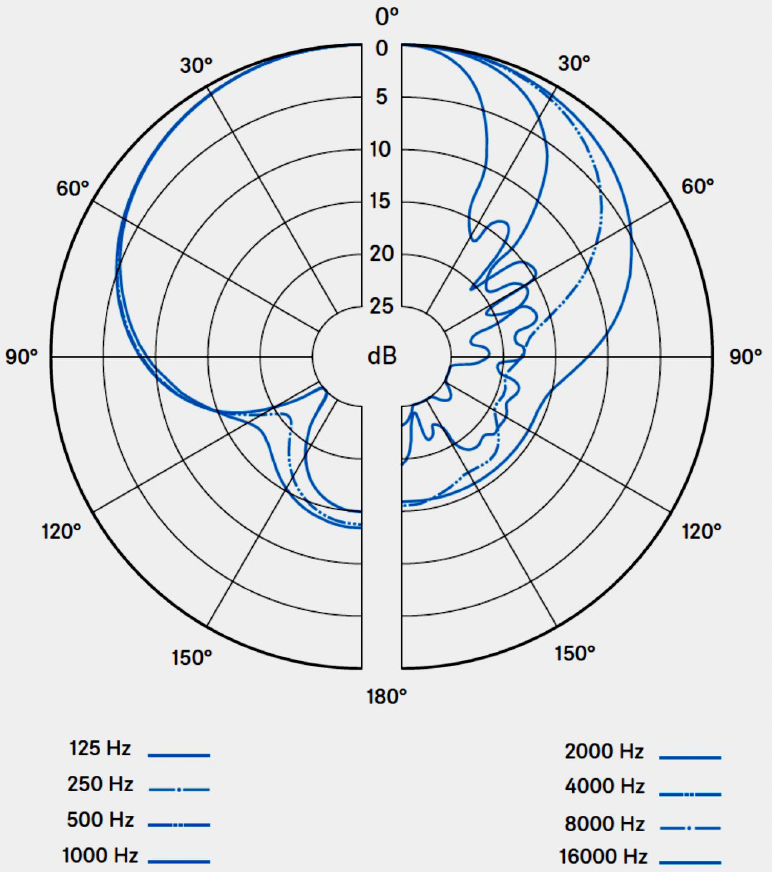
\includegraphics[width=0.33\linewidth]{highly_directional_mic.png}}
    \hfill
    \subfloat[Principle of the interference-tube assembly]{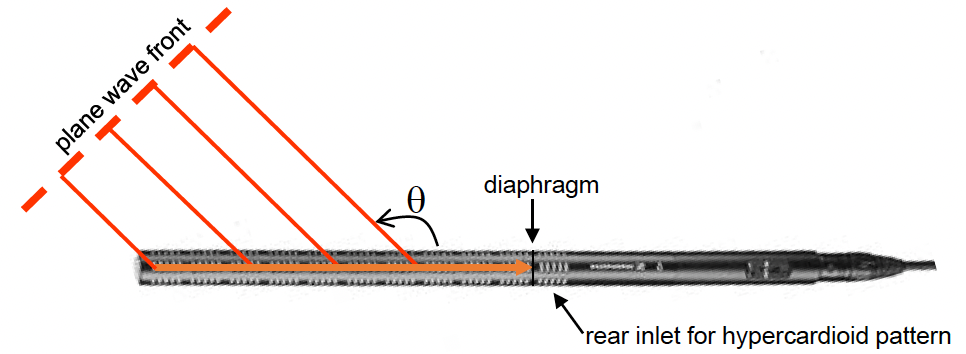
\includegraphics[height=0.15\textheight]{shotgun_mic_view.png}}
    \caption{Highly directional (shotgun) microphone: the interference tube narrows the main lobe strongly above the frequency at which the tube length exceeds half a wavelength, while a rear hypercardioid port maintains some rear rejection at low frequencies}
\end{figure}

\section{Frequency Response and Proximity Effect}
\label{sc:114}

\subsection{Relative Frequency Response}

The frequency response of a microphone quantifies how its sensitivity varies with the frequency of the incident sound.
It is defined as the relative sensitivity referred to the on-axis value at \SI{1}{\kilo\hertz}:
\[
S_{\mathrm{rel}}(f) = 20\log_{10}\left(\frac{S(f)}{S(\SI{1}{\kilo\hertz})}\right) \quad [\mathrm{dB}]
\]
An ideal microphone would exhibit \(S_{\mathrm{rel}}(f) = 0 \mathrm{dB}\) across the entire audio band from \SI{20}{\hertz} to \SI{20}{\kilo\hertz}, meaning that sensitivity is independent of frequency.
In practice, the response is bounded at the low end by the time constant of the static pressure equalization vent, which defines a high-pass cutoff below which the capsule ceases to respond to slowly varying pressure differences and at the high end by the finite relationship between the diaphragm diameter and the acoustic wavelength.

\subsection{Influence of Diaphragm Diameter}

The diaphragm diameter \(D\) governs a fundamental trade-off between sensitivity and upper frequency limit.
The sensitivity is proportional to the square of the diameter:
\[
S \propto D^2
\]
while the upper frequency at which a flat response is maintained is approximately inversely proportional to \(D\):
\[
f_{\mathrm{high}} \propto \frac{1}{D}
\]
A large diaphragm therefore delivers high sensitivity but a restricted high-frequency bandwidth, while a small diaphragm extends the flat band at the cost of reduced sensitivity.
Microphones of the same nominal diaphragm size can exhibit different sensitivities depending on the tension applied to the diaphragm during fabrication: lower tension increases mechanical compliance and raises sensitivity, while higher tension raises the resonance frequency and extends the high-frequency response.

\begin{figure}[!htb]
    \centering
    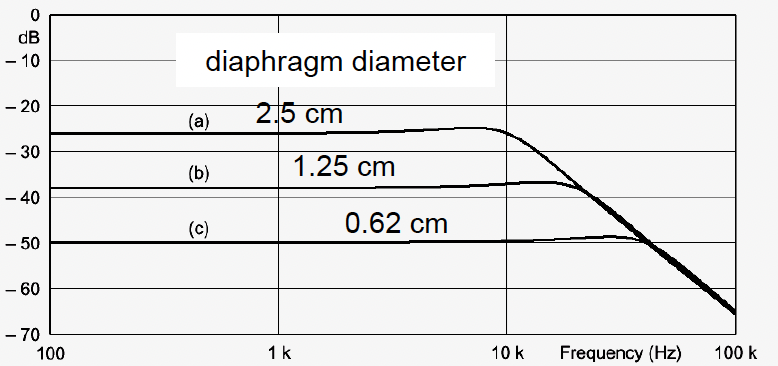
\includegraphics[width=0.65\textwidth]{diaphragm_diameter.png}
    \caption{Calculated frequency response magnitude for condenser capsules with diaphragm diameters of \SI{2.5}{\centi\meter}, \SI{1.25}{\centi\meter} and \SI{0.62}{\centi\meter} (curves a, b, c respectively): the flat band extends to progressively higher frequencies as the diaphragm is made smaller, at the expense of lower absolute sensitivity}
\end{figure}

\subsection{Proximity Effect}

Directional microphones, which sense the pressure difference across the two faces of the diaphragm, exhibit a characteristic low-frequency boost when the sound source is brought very close to the capsule.
This effect arises because the pressure gradient in the near field of a point source contains an additional \(1/r^2\) term beyond the far-field \(1/r\) contribution; at close distances this near-field gradient term becomes dominant and enhances the differential pressure driving the diaphragm at low frequencies, where the inter-face path difference constitutes a larger fraction of the wavelength.
The physical modeling of this mechanism is developed in detail in the following chapter; at this stage it suffices to note its practical consequence: as the source-to-microphone distance decreases below approximately \SI{30}{\centi\meter}, the low-frequency response rises progressively, producing a bass emphasis that grows more pronounced as the microphone is brought closer to the source.

\begin{figure}[!htb]
    \centering
    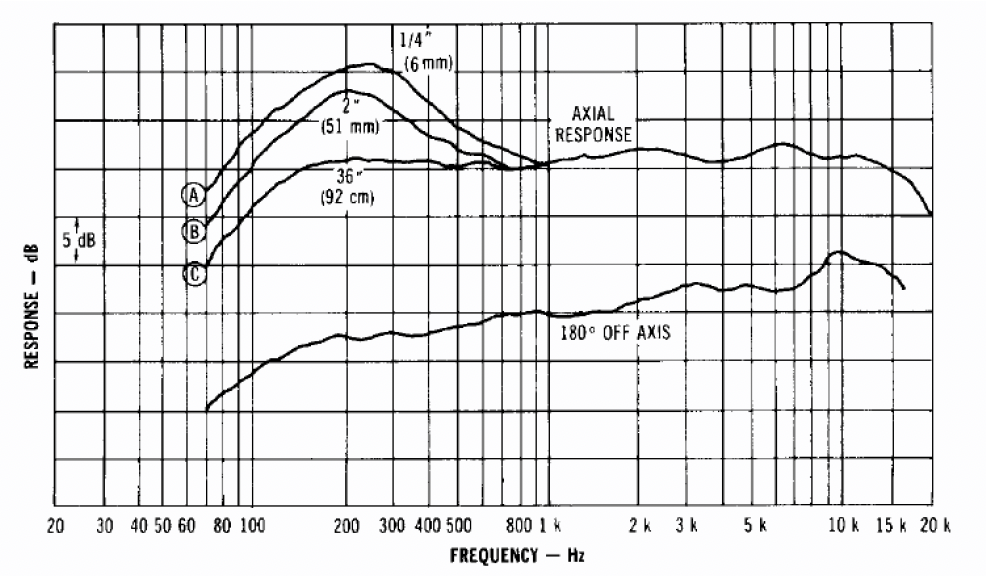
\includegraphics[width=0.65\textwidth]{proximity_effect.png}
    \caption{Position-dependent frequency response of a single-entry cardioid condenser microphone: the low-frequency response rises by several decibels as the source-to-microphone distance decreases from \SI{30}{\centi\meter} to \SI{7.5}{\centi\meter}, demonstrating the proximity effect}
\end{figure}

Many directional microphones intended for close-range vocal use are deliberately designed with a rolled-off low-frequency response at large distances, relying on the proximity effect to restore low-frequency energy when used close in, thereby achieving a balanced overall timbre.
In applications where proximity-effect coloration is undesirable, an internally switchable high-pass filter (often implementing a \SI{-6}{\decibel\per\octave} slope with a cutoff between \SI{80}{\hertz} and \SI{160}{\hertz}) allows the user to compensate.

\subsection{Static Pressure Equalization}

The static atmospheric pressure varies slowly over time due to weather changes and altitude differences at the recording site.
Even a change of \SI{1}{\milli\bar} corresponds to \SI{100}{\pascal}, a pressure \(10^8\) to \(10^9\) times larger than the faintest sound pressures to be captured; without compensation, such variations would displace the diaphragm far from its nominal rest position and fundamentally alter the capsule operating point.
To prevent this, every condenser capsule is equipped with a static pressure equalization vent, a narrow air channel connecting the internal cavity to the external atmosphere.
The vent allows the mean internal pressure to track the environmental static pressure with a time constant \(\tau\) set by the acoustic resistance and compliance of the channel, while leaving the acoustic signal band unaffected; the resulting low-frequency cutoff is:
\[
f_p = \frac{1}{2\pi \tau}
\]
For measurement microphones the time constant is typically \SI{0.1}{\second}, corresponding to a cutoff at approximately \SI{1.6}{\hertz}, which ensures a flat magnitude response down to below \SI{5}{\hertz} while filtering out all atmospheric drift.

\begin{figure}[!htb]
    \centering
    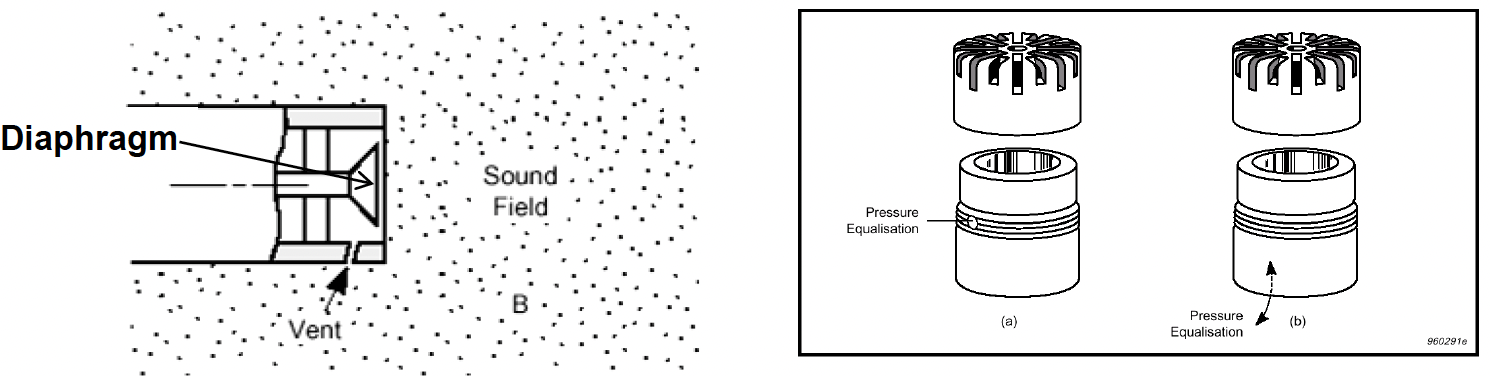
\includegraphics[width=0.65\textwidth]{mic_vent.png}
    \caption{Static pressure equalization vent in an omnidirectional condenser capsule: the narrow air channel (labeled B in the cross-section) connects the sealed rear cavity to the external atmosphere, allowing slow static pressure equalization while leaving the audio-band response unaffected}
\end{figure}

\subsection{Wind Noise and Protection}

Air flow across the microphone capsule generates turbulent pressure fluctuations at the diaphragm surface that are transduced as broadband noise, degrading the signal-to-noise ratio particularly at low frequencies.
This wind noise is distinct from acoustic noise in the sound field: it arises from the local aerodynamic boundary layer and is therefore not reproduced by headphone monitoring of a recording made simultaneously at a different position.
Three types of protection are commonly employed in practice: an internal wire-mesh windscreen integrated into the microphone grille, an external foam polyurethane slip-on windscreen that increases the effective turbulence distance from the diaphragm and an external pop filter (a stretched fabric membrane on a ring mount) positioned between the sound source and the microphone specifically to attenuate low-frequency plosive bursts from vocalists.

\begin{figure}[!htb]
    \centering
    \subfloat[Wind noise versus wind speed for windscreens of different diameters]{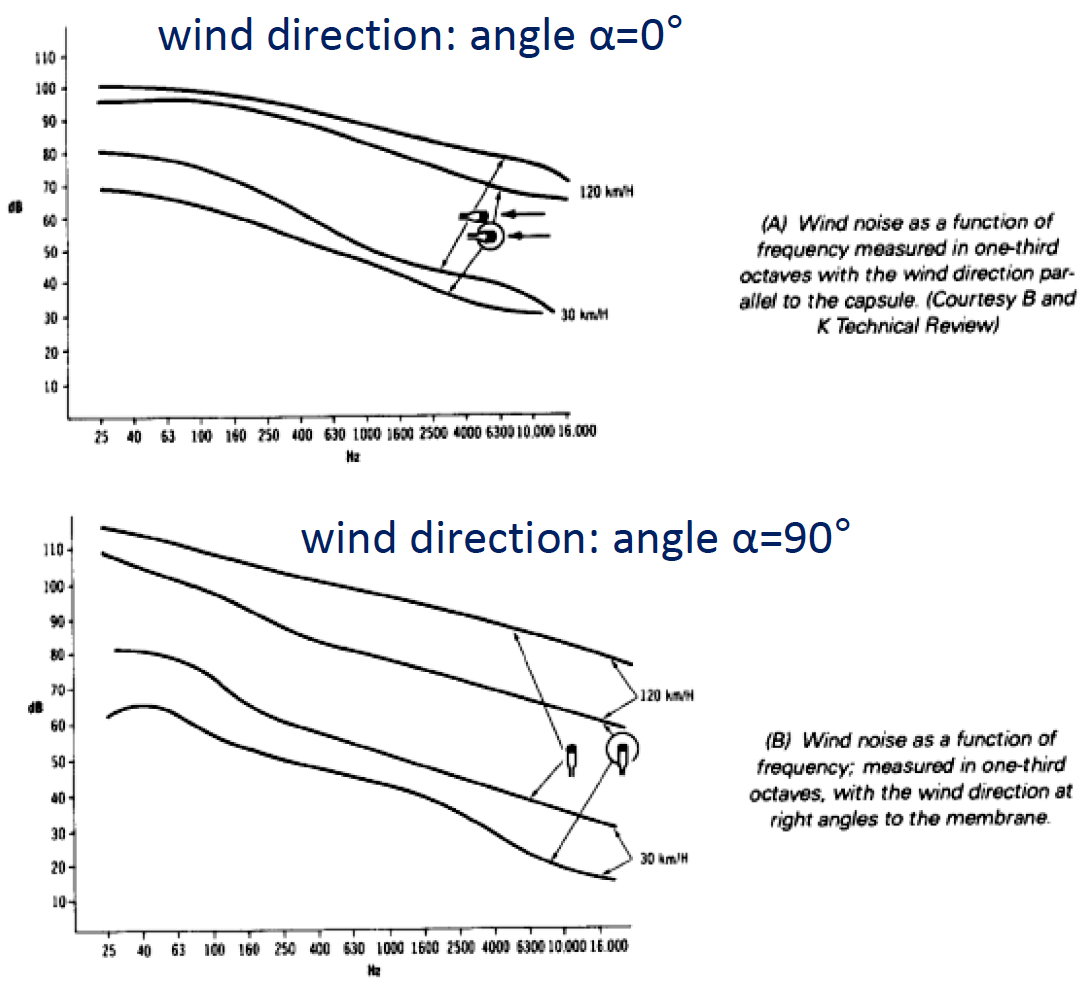
\includegraphics[height=0.25\textheight]{wind_noise_measurment.png}}
    \hfill
    \subfloat[Wind noise spectra at two wind directions]{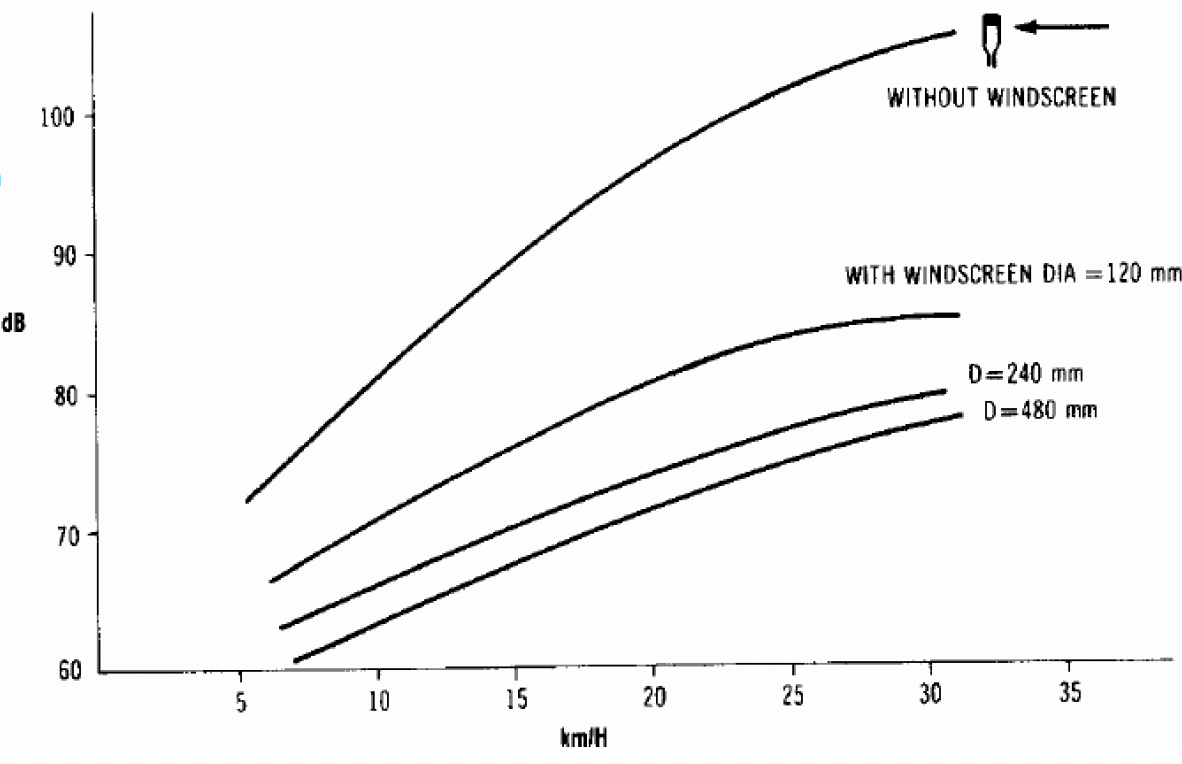
\includegraphics[height=0.25\textheight]{wind_noise.png}}
    \caption{Effect of windscreens on microphone noise: a larger windscreen body reduces turbulence-induced noise at a given wind speed, but all protection devices introduce some attenuation of the high-frequency signal response}
\end{figure}

\section{Noise and Dynamic Range}
\label{sc:115}

\subsection{Thermal Noise of the Microphone}

Even in a perfectly quiet acoustic environment, the microphone diaphragm is never at rest.
The thermal agitation of air molecules at finite temperature produces a continuous random bombardment of the diaphragm surface, inducing microscopic random displacements known as Brownian motion; these displacements are transduced into a fluctuating output voltage at the microphone terminals in the complete absence of any sound stimulus and constitute the irreducible lower limit of detectable acoustic pressure.
The noise voltage at the output can be referred back to the acoustic domain through the microphone sensitivity:
\[
p_{\mathrm{noise}} [\si{\pascal}_{\mathrm{RMS}}] = \frac{v_{\mathrm{noise}} [\si{\volt}_{\mathrm{RMS}}]}{S [\si{\volt\per\pascal}]}
\]
The resulting noise level is expressed in decibels relative to the standard reference pressure:
\[
\text{Noise level [dB SPL]} = 20\log_{10}\left(\frac{p_{\mathrm{noise}}}{\SI{20}{\micro\pascal}}\right)
\]
Typical self-noise values range from approximately \SI{0}{\decibel SPL} for large-diaphragm measurement-grade capsules to \SI{40}{\decibel SPL} for small-diaphragm designs.
For a condenser capsule, the noise pressure power spectral density is governed by the diaphragm mechanical parameters:
\[
\frac{\mathrm{d}P^2}{\mathrm{d}f} = 4kT \frac{2 \sigma t}{\pi R^4}
\]
where \(k\) is Boltzmann's constant, \(T\) is the absolute temperature, \(R\) is the diaphragm radius and \(\sigma t\) is the diaphragm tension per unit width.
Since the capsule sensitivity scales as \(R^2 / (\sigma t)\), the same design parameters that maximize sensitivity also minimize noise: both objectives simultaneously favor a large-area diaphragm operating at low tension.

\subsection{System Noise}

In any practical installation the microphone is connected to a preamplifier and the total system noise is the combined contribution of both sources.
At low frequencies the electronic noise of the preamplifier input stage typically dominates; at high frequencies the Brownian noise of the diaphragm becomes the limiting contribution, since the random displacement of the diaphragm grows relative to its signal displacement as the diaphragm area or tension decreases.

\begin{figure}[!htb]
    \centering
    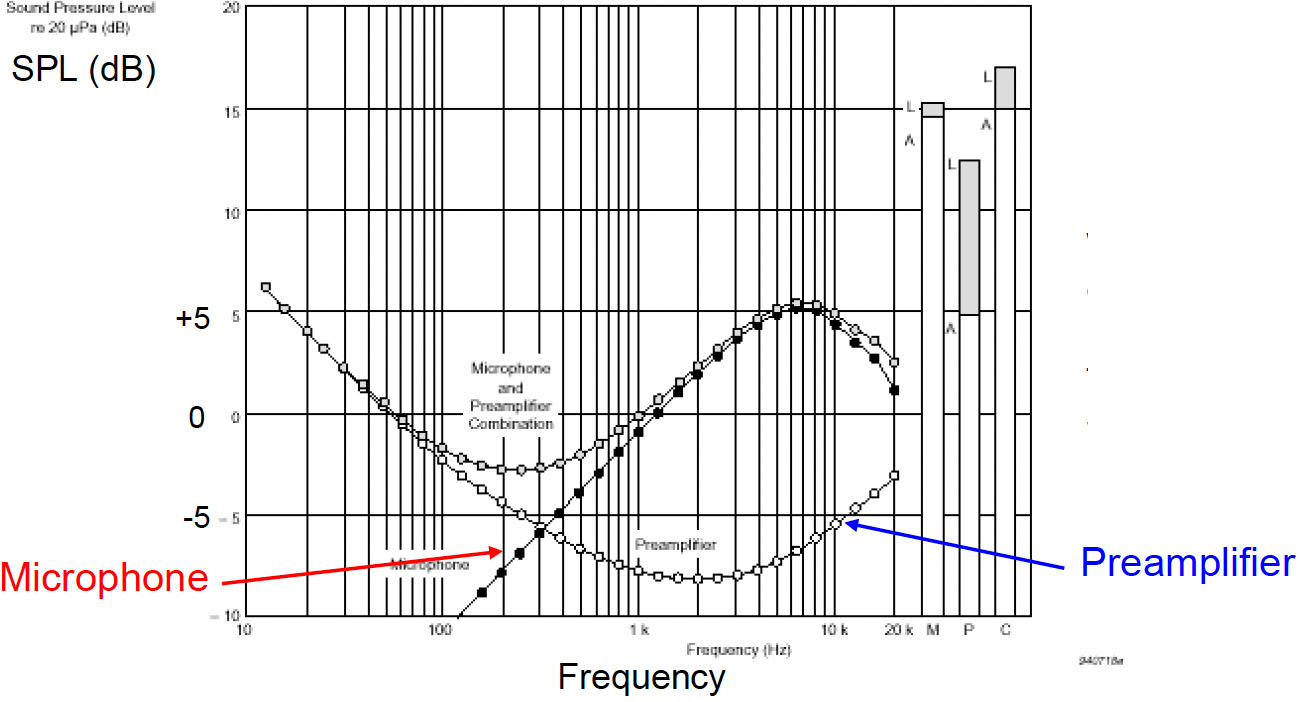
\includegraphics[width=0.75\textwidth]{mic_preamp_noise.png}
    \caption{Third-octave noise spectra of a complete measurement system consisting of a \(\tfrac{1}{2}''\) free-field condenser microphone (\SI{50}{\milli\volt\per\pascal}) and a high-quality preamplifier: preamplifier electronic noise dominates below approximately \SI{1}{\kilo\hertz}, while Brownian motion of the diaphragm sets the limit at high frequencies}
\end{figure}

This crossover behavior has practical design consequences: for low-noise recording of quiet sound sources, a large-diaphragm high-sensitivity capsule reduces the microphone's own noise contribution, while the preamplifier noise floor must be minimized independently; for demanding measurement applications, the sensitivity of the capsule also determines how much preamplifier gain is required, which in turn sets the amplifier's noise contribution referred to the input.

\subsection{Dynamic Range}

The dynamic range of a microphone is the interval between the minimum detectable sound pressure, set by the self-noise floor and the maximum allowable sound pressure, set by the onset of nonlinear distortion at a specified level.
The upper limit is conventionally quoted as the SPL at which the total harmonic distortion (THD) reaches \SI{1}{\percent} or \SI{3}{\percent}:
\[
\text{Dynamic Range} = \mathrm{SPL}_{\mathrm{max}} - \text{Noise level [dB SPL]}
\]
For the Shure KSM9 cited in section \ref{sc:112}, the self-noise is \SI{22}{\decibel SPL} (A-weighted) and the maximum SPL at \SI{1}{\percent} THD is \SI{152}{\decibel SPL}, yielding a dynamic range of \SI{130}{\decibel}.
High-performance measurement microphones can achieve dynamic ranges exceeding \SI{130}{\decibel}, enabling faithful capture of acoustic environments from the quietest anechoic chamber to the loudest aeroacoustic or industrial source without gain switching.

    %! TEX root = main.tex

\graphicspath{{00_Images/12_chapter/}}

\chapter{Condenser and MEMS Microphones}
\label{ch:condenser_mems}

\section{The Condenser Principle}
\label{sc:121}

The condenser (or capacitor) microphone is the most widely used transducer in precision measurement and studio recording, offering the best combination of flat frequency response, low self-noise, and extended bandwidth among all microphone types.
Its operating principle was first formalized by E.C. Wente in 1917 in a paper published in Physical Review, produced at the Research Laboratory of the American Telephone \& Telegraph Co. and Western Electric Co., where the device was described as a condenser transmitter for the absolute measurement of sound intensity.
The word transmitter reflected the primary application of the day: converting acoustic signals to electrical form for long-distance telephone transmission.
The theoretical treatment that followed in L.Beranek's textbook on acoustics established the electrostatic microphone as the standard for precision measurement, a role it retains today.

\subsection{Capacitance and Constant-Charge Operation}

A condenser microphone consists of a thin, tensioned diaphragm placed in close proximity to a rigid backplate, forming a parallel-plate capacitor whose capacitance varies with the instantaneous separation between the two electrodes.
The equilibrium capacitance is:
\[
C_0 = \varepsilon_0 \frac{A}{d_0}
\]
where \( A \) is the effective diaphragm area, \( d_0 \) is the rest-position gap, and \( \varepsilon_0 \) is the permittivity of free space.
The charge and voltage across the capacitor are linked by:
\[
Q = CV
\]
so that at equilibrium the bias voltage is \( V_B = Q_B / C_0 \), where \( Q_B \) is the bias charge placed on the capacitor.
The fundamental transduction principle is to maintain \( Q_B \) constant while the gap varies under acoustic pressure, so that any change in capacitance produces a proportional change in terminal voltage.
Holding the charge constant requires that the bias circuit present an extremely high impedance to the capsule: any charge leakage through a finite resistance \( R \) would discharge the capacitor on the time scale \( \tau = RC_0 \), and if \( \tau \) is comparable to the period of the audio signal, the low-frequency response degrades.

\subsection{Derivation of the Output Voltage}

When acoustic pressure \( p \) displaces the diaphragm by \( \Delta d \) toward the backplate, the new capacitance is:
\[
C = \varepsilon_0 \frac{A}{d_0 - \Delta d} \approx C_0 \left(1 + \frac{\Delta d}{d_0}\right)
\]
where the approximation holds for the small-signal regime \( |\Delta d| \ll d_0 \).
The incremental change in capacitance is therefore:
\[
\Delta C = C - C_0 \approx C_0 \frac{\Delta d}{d_0}
\]
With the charge held fixed at \( Q_B \), the new terminal voltage is \( V_B + V_S = Q_B/(C_0 + \Delta C) \), giving a signal voltage:
\begin{align*}
V_S &= Q_B\!\left(\frac{1}{C_0 + \Delta C} - \frac{1}{C_0}\right)
= Q_B \frac{-\Delta C}{C_0(C_0 + \Delta C)} \\
&\approx -\frac{Q_B}{C_0}\frac{\Delta C}{C_0}
= -V_B \frac{\Delta C}{C_0}
\end{align*}
Substituting the expression for \( \Delta C \):
\[
V_S \approx -V_B \frac{\Delta C}{C_0} \approx V_B \frac{\Delta d}{d_0}
\]
A displacement toward the backplate (compression) increases the capacitance and decreases the terminal voltage, consistent with the negative sign before \( \Delta C / C_0 \).
The signal voltage is therefore directly proportional to the diaphragm displacement, as illustrated in figure \ref{fig:condenserCrossSection}.

\begin{figure}[!htb]
    \centering
    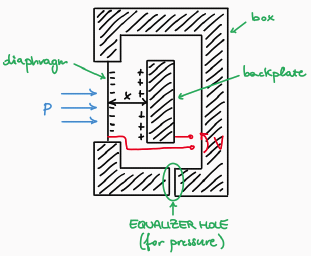
\includegraphics[width=0.55\textwidth]{condenser_mic.png}
    \caption{Simplified cross-section of a condenser microphone capsule: the tensioned diaphragm and the rigid backplate form a variable capacitor, and the vent hole provides static pressure equalization at the rear of the diaphragm}
    \label{fig:condenserCrossSection}
\end{figure}

\subsection{Stiffness-Controlled Regime and Sensitivity}

At audio frequencies well below the diaphragm resonance, the displacement is governed by the elastic restoring force of the diaphragm rather than by its inertia, so the system operates in the stiffness-controlled regime.
The displacement is proportional to the applied force:
\[
\Delta d = C_{MS}F = C_{MS}pS_D
\]
where \( C_{MS} \) is the mechanical compliance of the diaphragm.
Substituting into the signal voltage expression and using \( V_B/d_0 = Q_B/(\varepsilon_0A) \):
\[
V_S = \frac{Q_B}{\varepsilon_0A}C_{MS}pS_D = \frac{Q_B}{\varepsilon_0}C_{MS}p
\]
since \( A \equiv S_D \).
The open-circuit sensitivity of the condenser microphone is therefore:
\[
\mathcal{S} = \frac{V_S}{p} = \frac{Q_B}{\varepsilon_0}C_{MS}
\]
The sensitivity increases with the bias charge and with the mechanical compliance of the diaphragm.
A softer diaphragm produces a larger displacement for a given pressure, yielding higher sensitivity; conversely, a stiffer diaphragm raises the resonance frequency and extends the flat response region.
This stiffness-controlled operation contrasts with the electrodynamic loudspeaker, which operates in a mass-controlled regime above its mechanical resonance.

\begin{figure}[!htb]
    \centering
    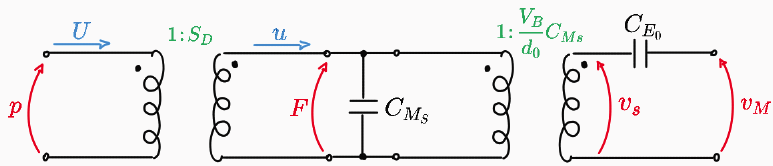
\includegraphics[width=0.70\textwidth]{condenser_mic_equiv_circuit.png}
    \caption{Equivalent electromechanical circuit of the condenser capsule: acoustic pressure \( p \) produces the force \( F = pS_D \) acting on the diaphragm compliance \( C_{MS} \), and the resulting displacement modulates the electrical capacitance \( C_{E0} \) to produce the output signal voltage}
\end{figure}

\subsection{Electret Microphones}

A standard condenser microphone requires an external bias voltage, typically \SI{48}{\volt} of phantom power, to establish the charge \( Q_B \) on the capsule.
An electret microphone eliminates this external requirement by permanently polarizing the backplate or the diaphragm with a dielectric material that retains a built-in electrostatic charge.
The backplate is coated with a fluoropolymer film, typically fluorinated ethylene propylene (FEP): during manufacture the material is heated above its glass transition temperature, subjected to a strong electric field, and cooled with the field applied, freezing the aligned molecular dipoles in place and creating a permanently embedded surface charge equivalent to the external bias.

\begin{figure}[!htb]
    \centering
    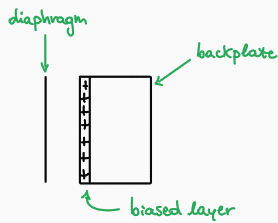
\includegraphics[width=0.35\textwidth]{electret_mic_structure.png}
    \caption{Cross-section of an electret capsule: the permanently polarized dielectric layer on the backplate supplies the bias charge \( Q_B \) without requiring an external polarization supply}
\end{figure}

The sensitivity expression \( \mathcal{S} = Q_BC_{MS}/\varepsilon_0 \) applies identically to electret and externally polarized designs; the only distinction is the source of \( Q_B \).
An internal impedance converter is still required to extract the signal from the high-impedance capsule, and it is powered via phantom power or a small internal battery.
Modern electret capsules achieve performance virtually indistinguishable from externally polarized types and represent the large majority of condenser microphones produced, including essentially all consumer, communication, and MEMS devices.

\section{Internal Electronics and Phantom Power}
\label{sc:122}

The condenser capsule presents a source impedance that is nearly that of a pure capacitance of a few picofarads, which at audio frequencies corresponds to a source impedance on the order of hundreds of megaohms.
This extremely high impedance makes the signal vulnerable to loading by any parasitic capacitance in the signal path before the first amplifying stage.

\subsection{The Cable Capacitance Problem}

When the microphone capsule is connected to a cable without an internal buffer, the capsule capacitance \( C_{E0} \) forms a capacitive voltage divider with the sum of the cable capacitance and the preamplifier input capacitance.
Typical values for a professional installation are:
\[
C_{E0} \approx \SI{10}{\pico\farad}, \qquad
C_{\mathrm{IN}} \approx \SI{10}{\pico\farad}, \qquad
C_{\mathrm{cable}} \approx \SI{100}{\pico\farad\per\meter}
\]
For a cable of length \( l = \SI{1}{\meter} \), the fraction of the signal recovered at the preamplifier input is:
\[
\frac{v_{\mathrm{IN}}}{v_s} = \frac{C_{E0}}{C_{E0} + C_{\mathrm{cable}}l + C_{\mathrm{IN}}}
= \frac{10}{10 + 100 + 10}
\approx \frac{1}{12}
< 10\%
\]
More than \SI{90}{\percent} of the signal is dissipated in the capacitive divider before it reaches the preamplifier, an unacceptable loss for any precision audio system.

\begin{figure}[!htb]
    \centering
    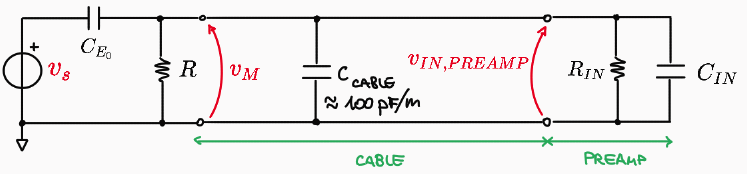
\includegraphics[width=0.60\textwidth]{microphone_cable_effect.png}
    \caption{Capacitive loading of the unshielded condenser capsule: the capsule capacitance \( C_{E0} \), the cable capacitance \( C_{\mathrm{cable}} \), and the preamplifier input capacitance \( C_{\mathrm{IN}} \) form a voltage divider; without an internal buffer, a \SI{1}{\meter} cable recovers less than 10\% of the signal}
\end{figure}

The solution is to integrate an impedance converter, typically a JFET source follower, directly inside the microphone body and as close to the capsule as physically possible.
The JFET gate presents an input impedance in excess of \SI{1}{\giga\ohm} to the capsule, and the source presents a low output impedance of a few hundred ohms to the cable.
With the buffer in place, the cable capacitance loads the JFET output rather than dividing the capsule voltage directly, and the signal attenuation becomes negligible.
A large bias resistor \( R_B \), typically several hundred megaohms, establishes the DC gate potential and forms a high-pass RC network with the capsule capacitance; the cutoff frequency is:
\[
f_L = \frac{1}{2\pi R_BC_{E0}}
\]
For \( C_{E0} = \SI{10}{\pico\farad} \) and the requirement \( f_L \leq \SI{20}{\hertz} \), the minimum bias resistance is:
\[
R_B \geq \frac{1}{2\pi \cdot \SI{20}{\hertz} \cdot \SI{10}{\pico\farad}} \approx \SI{800}{\mega\ohm}
\]

\begin{figure}[!htb]
    \centering
    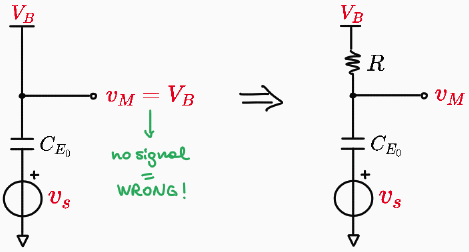
\includegraphics[width=0.50\textwidth]{electret_mic_bias_circuit.png}
    \caption{Bias and coupling circuit for signal extraction from a condenser capsule: the large resistor \( R_B \) establishes the JFET gate potential while the coupling capacitor isolates the AC signal; the RC network functions as a high-pass filter with cutoff \( f_L = 1/(2\pi R_B C_{E0}) \)}
\end{figure}

\subsection{Phantom Power}

The internal impedance converter and any subsequent preamplifier stages require an operating voltage.
Rather than a separate power cable or internal battery, professional condenser microphones use phantom power: the operating voltage is delivered over the same balanced cable that carries the audio signal, completely transparent to the audio system.
The standard phantom supply voltage is \( V_{\mathrm{BIAS}} = \SI{48}{\volt} \) (IEC 61938), though voltages between \SI{11}{\volt} and \SI{52}{\volt} are found in practice depending on the application.
The supply voltage is applied to the center tap of the output transformer inside the microphone, or equivalently through two equal resistors connected to pins 2 and 3 of the XLR connector in a transformerless design.
Both signal conductors carry the same DC potential \( V_{\mathrm{BIAS}} \) with respect to the shield, and the total current \( I \) consumed by the preamplifier divides equally as \( I/2 \) in each conductor.
At the preamplifier end, the differential input amplifies only the voltage difference between the two conductors: since both carry the same DC level, the phantom supply produces no net differential signal, and it does not appear at the audio output.

\begin{figure}[!htb]
    \centering
    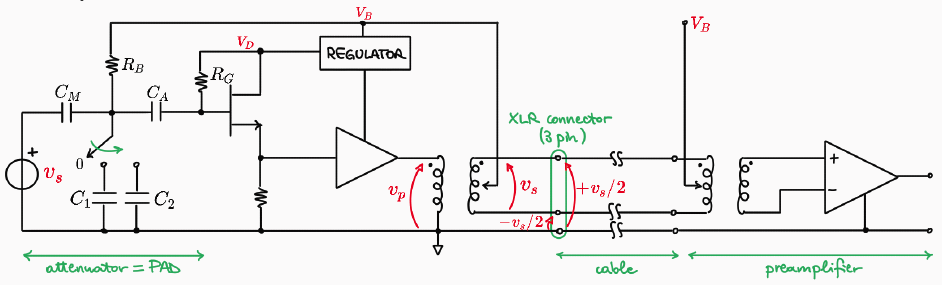
\includegraphics[width=0.85\textwidth]{phantom_power.png}
    \caption{Phantom power circuit architecture: the bias voltage \( V_{\mathrm{BIAS}} \) is fed symmetrically to both signal conductors through equal resistors; the stationary current \( I \) splits as \( I/2 \) in each leg, supplying power to the internal preamplifier without appearing as a differential audio signal}
\end{figure}

\paragraph{Common-mode rejection of supply disturbances} Consider a disturbance current \( i \) superimposed on the nominal supply current, arising for instance from power-supply ripple or electromagnetic pickup on the cable.
Because the phantom topology is symmetric, the disturbance distributes equally as \( i/2 \) in each conductor, producing an identical voltage perturbation \( v/2 \) on both lines.
The differential voltage presented to the preamplifier input is:
\[
v_{\mathrm{diff}}
= \left(V_{\mathrm{BIAS}} + \frac{v}{2}\right)
- \left(V_{\mathrm{BIAS}} + \frac{v}{2}\right) = 0
\]
The disturbance is a pure common-mode signal and is rejected by the differential amplifier stage.
The common-mode rejection ratio (CMRR) of professional microphone preamplifiers is typically \SI{60}{\decibel} or higher across the audio band, attenuating the residual interference by a factor of at least 1000.
This is the fundamental advantage of the balanced differential connection used in all professional audio installations: any electromagnetic interference induced equally on both conductors cancels at the differential input, while the desired audio signal, which is transmitted as a differential voltage \( +v_s/2 \) on one conductor and \( -v_s/2 \) on the other, is unaffected.

\begin{figure}[!htb]
    \centering
    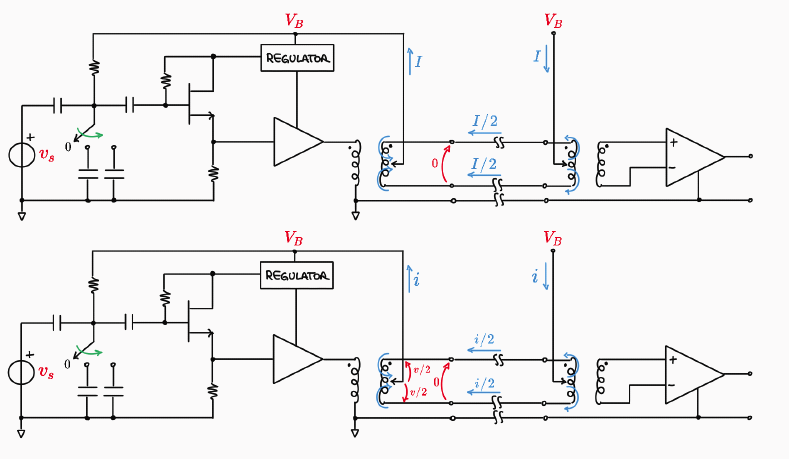
\includegraphics[width=0.85\textwidth]{phantom_power_2.png}
    \caption{Common-mode rejection in the phantom power line: the stationary supply current \( I \) and a superimposed disturbance \( i \) both distribute symmetrically as \( (I+i)/2 \) on each conductor; the disturbance voltages \( v/2 \) appear identically on both lines and cancel at the differential preamplifier input, leaving the audio signal intact}
\end{figure}

\subsection{Complete Internal Electronics Chain}

A representative internal electronics chain, exemplified by designs such as the Shure SM81 or the AKG C-460B, includes the following functional stages in cascade: a capacitive attenuator pad for operation at high sound pressure levels up to \SI{145}{\decibel} SPL; a JFET source follower as the primary impedance converter; a passive high-pass RC filter network providing switchable low-frequency roll-off (flat, \SI{-6}{\decibel\per\octave} at \SI{100}{\hertz}, or \SI{-18}{\decibel\per\octave} at \SI{80}{\hertz}); a BJT buffer for additional current drive capacity; and an output transformer that converts the single-ended capsule signal to a balanced differential output while injecting the phantom supply voltage at its center tap.
In transformerless designs, the balanced output is produced by a symmetric active output stage followed by two DC-blocking capacitors, and the phantom voltage is injected through two matched resistors directly at the connector.
Every component in the high-impedance node preceding the JFET gate must be designed for minimum thermal noise, since even a single resistor at this node can dominate the noise floor of the entire microphone.


\section{MEMS Microphones}
\label{sc:123}

Micro-Electro-Mechanical Systems (MEMS) microphones represent the most recent evolution of the condenser transduction principle and now constitute the dominant microphone technology by units produced worldwide.
By applying the photolithographic fabrication techniques of integrated circuit manufacturing to acoustic transducers, MEMS technology enables the production of complete microphone capsules at the scale and per-unit cost of passive electronic components, with dimensional control at the sub-micrometer level.

\subsection{The MEMS Concept}

MEMS is the integration of mechanical elements, sensors, actuators, and electronics on a common silicon substrate through microfabrication technology.
The electronic components are fabricated using standard IC process sequences such as CMOS, Bipolar, or BiCMOS, while the micromechanical structures are produced by compatible micromachining processes that selectively etch away regions of the silicon wafer or deposit new structural layers to form movable mechanical elements.
In the context of microphones, the mechanical element is a thin silicon diaphragm suspended above a rigid perforated backplate, reproducing the diaphragm-and-backplate geometry of a conventional condenser capsule at a scale of hundreds of micrometers.

\subsection{Silicon Microfabrication Technology}

The starting material for all silicon microfabricated devices is a monocrystalline silicon wafer of electronic-grade purity.
Metallurgic-grade silicon, obtained by reducing silicon dioxide with carbon in an arc furnace:
\[
\mathrm{SiC(s)} + \mathrm{SiO_2(s)} \longrightarrow \mathrm{Si(s)} + \mathrm{SiO(g)} + \mathrm{CO(g)}
\]
achieves a purity of approximately 98\%, which is insufficient for electronic applications.
Further purification to electronic grade reduces the total impurity concentration (boron, copper, gold, iron, chromium, manganese, and others) to below \( 10^{13} \) atoms per \si{\centi\meter\cubed}, against a silicon atom concentration of \( 10^{22} \) atoms per \si{\centi\meter\cubed}, corresponding to a purity of \( 10^{-3} \) ppm, or 99.9999999\%.
Monocrystalline ingots are grown from this purified material by the Czochralski process: a small seed crystal is dipped into a quartz crucible containing molten silicon held at the silicon fusion temperature of \( \SI{1415}{\degreeCelsius} \), then slowly withdrawn and rotated, pulling a single-crystal ingot with a diameter between \SI{4}{\inch} and \SI{12}{\inch}.
The ingot is sliced into wafers of thickness between \SI{300}{\micro\meter} and \SI{500}{\micro\meter}, which are then lapped and polished to a surface flatness variation below \SI{1}{\micro\meter}, providing the planar substrate required for photolithographic processing.
The primary microfabrication steps applied to each wafer are as follows.

\paragraph{Thermal oxidation} Heating the wafer in an oxidizing atmosphere grows a conformal layer of silicon dioxide (\(\mathrm{SiO_2}\)) by consuming the silicon surface; this oxide serves as an electrical insulator, a diffusion mask for subsequent doping steps, and a sacrificial layer that can be selectively removed later to release mechanical structures.

\paragraph{Photolithography} A photosensitive polymer (photoresist) is spin-coated onto the wafer, exposed through a reticle carrying the desired pattern using ultraviolet light, and developed to reveal the exposed areas; the resulting patterned mask protects selected regions during etching, enabling the definition of features with lateral dimensions below one micrometer.

\paragraph{Etching} Both wet chemical etching using solutions such as KOH for anisotropic silicon removal and HF for silicon dioxide, and dry plasma etching using reactive ion processes, are employed to sculpt the three-dimensional microstructure; in MEMS acoustic devices, a deep anisotropic etch through the full wafer thickness forms the back cavity that acoustically loads the diaphragm and defines the backvolume of the capsule.
After all structural and electrical layers have been deposited and patterned, a final release etch removes the sacrificial oxide beneath the diaphragm, freeing it from the substrate and leaving it suspended above the backplate by an air gap of precisely controlled thickness.

\subsection{MEMS Microphone Structure and Fabrication Routes}

A MEMS microphone capsule reproduces, at microscale, the diaphragm-and-backplate geometry of a conventional condenser capsule.
The diaphragm is a thin circular membrane of LPCVD (low-pressure chemical vapor deposited) silicon nitride or polysilicon, typically \SI{0.5}{\micro\meter} to \SI{2}{\micro\meter} thick, deposited under controlled conditions to achieve a prescribed residual tensile stress that governs its compliance and resonance frequency.
The backplate is a rigid electrode perforated with acoustic holes that allow air to flow freely through the gap, preventing the sealed air volume from acting as an additional stiffness in series with the diaphragm suspension.
Two main fabrication routes are used in practice.
In the two-wafer bonding process, the diaphragm and backplate are fabricated independently on two separate wafers: the diaphragm wafer undergoes oxide formation, silicon nitride deposition, and electrode patterning, while the backplate wafer is etched to define the acoustic holes and stiffening geometry; the two wafers are then bonded face-to-face by gold-gold thermocompression bonding, and the bonding pad height defines the air gap with sub-micrometer accuracy.
In the single-wafer surface micromachining process, a sacrificial oxide layer deposited at the start of the process defines the future gap thickness; polysilicon or silicon nitride is deposited on top to form the diaphragm; a final vapor-HF or wet-HF etch removes the sacrificial layer through the acoustic holes in the backplate, releasing the diaphragm on the same substrate without wafer bonding.

\subsection{Sensitivity and the Role of the Air Gap}

The key performance advantage of MEMS microphones originates directly from the small air gap dimension made possible by photolithographic processing.
The electrostatic pressure acting on the diaphragm per unit area, derived from the energy stored in the electric field, is:
\[
P_{\mathrm{el}} = \frac{\varepsilon_0V_B^2}{2d^2} \propto \frac{1}{d^2}
\]
Reducing the gap by a factor of ten at the same bias voltage increases the electrostatic force by a factor of one hundred.
The electric field \( \mathcal{E} = V_B/d \) scales inversely with gap, and the charge-to-voltage conversion efficiency \( V_S/\Delta d = V_B/d \) also scales inversely with gap, so a ten-fold reduction in gap yields a ten-fold improvement in sensitivity for the same diaphragm displacement.
In a conventional condenser capsule, the gap between diaphragm and backplate is typically on the order of \SI{20}{\micro\meter} to \SI{50}{\micro\meter}, limited by mechanical tolerances in the hand-assembly process.
In a MEMS device, the gap is defined by a deposited sacrificial oxide layer with a thickness of \SI{1}{\micro\meter} to \SI{4}{\micro\meter}, controlled to sub-micrometer accuracy by the deposition recipe.
This is the fundamental reason why MEMS microphones achieve sensitivity values comparable to much larger conventional capsules despite their millimeter-scale diaphragm area: the sub-micrometer gap generates an intense electric field from a modest bias voltage, compensating for the reduced electrode area.

\subsection{Commercial MEMS Microphones}

Commercial MEMS microphones are available in two output formats distinguished by the level of signal processing performed on-chip.
Analog MEMS microphones produce a continuous voltage output proportional to acoustic pressure; they include an on-chip JFET or CMOS impedance converter but no analog-to-digital conversion, and they interface to standard audio signal chains with supply voltages between \SI{1.5}{\volt} and \SI{5.5}{\volt} and current consumptions below \SI{250}{\micro\ampere}.
Digital MEMS microphones integrate a sigma-delta modulator alongside the MEMS capsule on the same die, producing a single-bit Pulse Density Modulation (PDM) bitstream at a clock frequency between \SI{1}{\mega\hertz} and \SI{4}{\mega\hertz}; this bitstream is decoded by an audio codec, DSP, or microcontroller, eliminating all analog conditioning in the downstream system and providing inherent immunity to electromagnetic interference on the signal lines.
The key practical advantages of MEMS microphones over conventional condenser capsules include their compact package size, with footprints on the order of \( 3\mathrm{mm} \times 4\mathrm{mm} \times 1\mathrm{mm} \); compatibility with automated surface-mount reflow soldering at temperatures up to \SI{260}{\degreeCelsius}, which eliminates hand-assembly; high resistance to mechanical shock; and exceptional unit-to-unit matching.
Because thousands of capsules are fabricated simultaneously on a single wafer under identical photolithographic conditions, matched pairs selected from the same batch exhibit sensitivity differences below \SI{1}{\decibel}, making MEMS microphones the enabling technology for stereo arrays, beamforming systems, and differential noise-cancellation configurations in smartphones, laptops, hearing aids, wearable devices, and industrial IoT sensors.

    %! TEX root = main.tex

\graphicspath{{00_Images/13_chapter/}}

\chapter{Microphone Directivity and Models}

Microphones are classified according to the acoustic quantity they sense: the absolute pressure at a point, the spatial gradient of that pressure, or a weighted combination of both.
This distinction determines not only the directional response but also the sensitivity to source distance, and it underpins the design of every practical microphone pattern from the omnidirectional to the hypercardioid.

\section{Pressure Microphones}

A pressure microphone exposes only one face of its diaphragm to the sound field; the rear face is enclosed by a sealed cavity.
A narrow equalization vent connects the interior of that cavity to the ambient atmosphere, allowing slow static pressure changes to pass through without affecting the audio-band response, while remaining acoustically opaque to acoustic frequencies.
The incident plane wave \(\tilde{p} = \tilde{p}_0 e^{-jkx}\) acts directly on the exposed face, and the net driving force on a diaphragm of area \(S_D\) is simply
\[
\tilde{f}_D = \tilde{p} S_D
\]
Because the rear cavity is sealed, only the absolute pressure on the front face matters; the differential pressure across the diaphragm equals the incident pressure itself.

\begin{figure}[!htb]
    \centering
    \subfloat[Cross-section of a pressure-microphone capsule with equalization vent]{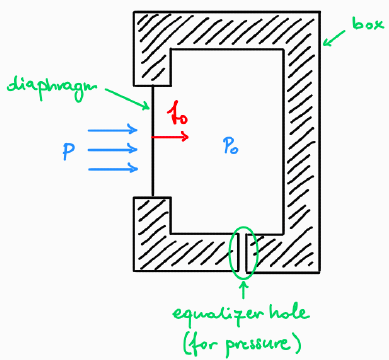
\includegraphics[height=0.2\textheight]{pressure_mic_structure.png}}
    \hfill
    \subfloat[Omnidirectionality condition: when \(\lambda \gg L\) the pressure is spatially uniform across the diaphragm]{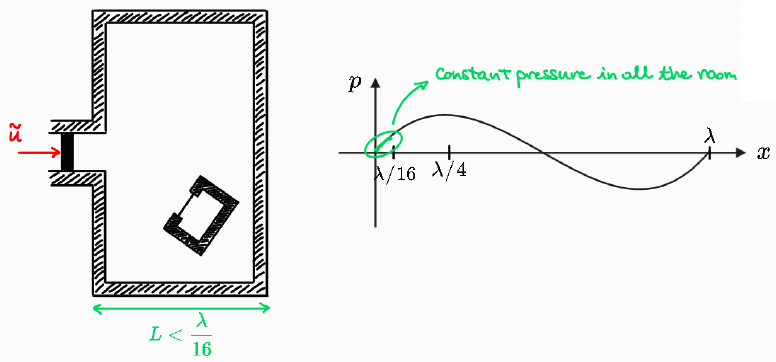
\includegraphics[height=0.2\textheight]{room.png}}
    \caption{Pressure microphone: capsule structure and the long-wavelength condition that guarantees omnidirectional response}
\end{figure}

As long as the acoustic wavelength \(\lambda\) is much larger than the microphone body (dimension \(L\)), the pressure does not vary appreciably from one side of the diaphragm to the other, and the output voltage is independent of the angle of incidence \(\theta\):
\[
v_P(\theta) = v_{P0}
\]
The pressure microphone is therefore inherently omnidirectional.
At high frequencies, where the microphone body becomes comparable to the wavelength, diffraction creates an acoustic shadow and the directional response departs from the circular polar pattern; this sets an upper frequency limit that scales inversely with capsule diameter, as discussed in the previous chapter on specifications.

\section{Pressure-Gradient Microphones}

A pressure-gradient microphone exposes both faces of the diaphragm directly to the sound field.
The diaphragm therefore responds to the pressure difference \(\tilde{p}_1 - \tilde{p}_2\) across its two sides, which is proportional to the local spatial derivative of the pressure field.
This differential coupling makes the transducer inherently directional.

\subsection{Force on the Diaphragm: Plane-Wave Excitation}

Let \(\tilde{p}_1\) and \(\tilde{p}_2\) denote the acoustic pressures at the front and rear faces of the diaphragm, separated along the acoustic axis by an effective path distance \(\Delta l\).
The net acoustic force on the diaphragm, projected onto its normal, is
\[
\tilde{f}_{D\perp} = (\tilde{p}_1 - \tilde{p}_2) S_D \cos\theta
\]
where \(\theta\) is the angle of incidence measured from the diaphragm axis, so that on-axis incidence corresponds to \(\theta = 0\).

\begin{figure}[!htb]
    \centering
    \subfloat[Differential pressure acting on the two faces of the diaphragm]{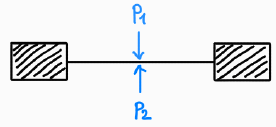
\includegraphics[height=0.18\textheight]{pressure_grad_mic_1.png}}
    \hfill
    \subfloat[Plane wave at angle \(\theta\) and the effective path difference \(\Delta l\) across the diaphragm]{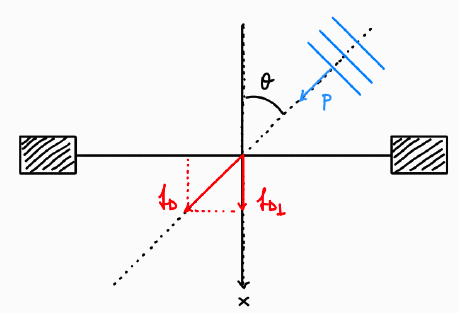
\includegraphics[height=0.18\textheight]{pressure_grad_mic_plane.png}}
    \caption{Pressure-gradient microphone: forces on the diaphragm faces and the geometry of oblique incidence}
\end{figure}

For small separations \(\Delta l\), the pressure difference is approximated to first order as
\[
\tilde{p}_1 - \tilde{p}_2 \approx -\frac{\partial \tilde{p}}{\partial x} \Delta l
\]
giving
\[
\tilde{f}_{D\perp} = -S_D \frac{\partial \tilde{p}}{\partial x} \Delta l \cos\theta
\]
The acoustic momentum equation (Newton's second law applied to a fluid element) relates the pressure gradient to the particle velocity:
\[
-\frac{\partial p}{\partial x} = \rho_0 \frac{\partial u}{\partial t}
\]
For harmonic excitation \(\tilde{u} = u_0 e^{j\omega t}\), the time derivative yields \(\partial\tilde{u}/\partial t = j\omega \tilde{u}\), so the normal force becomes
\[
\tilde{f}_{D\perp} = \rho_0 S_D \Delta l j\omega \tilde{u} \cos\theta = jk \rho_0 c \tilde{u} S_D \Delta l \cos\theta
\]
For a plane wave, \(\partial\tilde{p}/\partial x = -jk \tilde{p}\), which permits the force to be expressed directly in terms of pressure:
\[
\tilde{f}_{D\perp} = jk \tilde{p} S_D \Delta l \cos\theta, \qquad |\tilde{f}_{D\perp}| = \frac{\omega}{c} |\tilde{p}| S_D \Delta l |\cos\theta|
\]
The angular dependence \(|\cos\theta|\) implies that the response is maximum on-axis (\(\theta = 0^\circ\)), vanishes at \(\theta = \pm 90^\circ\), and reappears with opposite sign at \(\theta = 180^\circ\): the output voltage follows \(v_G(\theta) = v_{G0}\cos\theta\), which is the bidirectional or figure-eight polar pattern.

\begin{figure}[!htb]
    \centering
    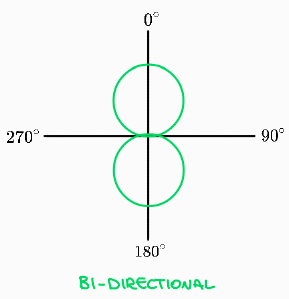
\includegraphics[width=0.38\textwidth]{bi_directional_pattern.png}
    \caption{Bidirectional (figure-eight) polar pattern of a pressure-gradient microphone for plane-wave excitation}
\end{figure}

\paragraph{Effective path difference} The value of \(\Delta l\) is set by the radiation impedance of the diaphragm rather than by its physical size alone.
For a rigid circular diaphragm of radius \(a\) acting as a piston in free space, the specific radiation impedance at low frequencies gives
\[
\Delta l_{\mathrm{rigid}} = \frac{4a}{3\pi} \approx \frac{a}{2}
\]
For a flexible disk vibrating in its first bending mode, the radiation impedance yields a somewhat larger effective path:
\[
\Delta l_{\mathrm{flex}} = \frac{\pi a}{4} \approx \frac{3a}{4}
\]
Both limiting cases confirm that \(\Delta l\) is of order \(a\), the diaphragm radius.

\subsection{Force on the Diaphragm: Spherical Waves and the Proximity Effect}

When the acoustic source is a point monopole at distance \(r\), the pressure field is spherical:
\[
\tilde{p}(r) = \tilde{A}_0 \frac{e^{-jkr}}{r}
\]
The radial pressure gradient is then
\[
\frac{\partial \tilde{p}}{\partial r} = -\frac{1+jkr}{r} \tilde{p}(r)
\]
and the normal diaphragm force becomes
\[
\tilde{f}_{D\perp} = \tilde{p}(r) \frac{1+jkr}{r} S_D \Delta l \cos\theta
\]
Taking the RMS magnitude and using the spherical-wave relation \(|\tilde{u}|_{\mathrm{rms}} = |\tilde{p}|_{\mathrm{rms}} \sqrt{1+(kr)^2} /(kr \rho_0 c)\):
\[
|\tilde{f}_{D\perp}|_{\mathrm{rms}} = |\tilde{p}|_{\mathrm{rms}} \frac{\sqrt{1+(kr)^2}}{r} \frac{\omega}{c} S_D \Delta l \cos\theta = |\tilde{u}|_{\mathrm{rms}} \omega \rho_0 S_D \Delta l \cos\theta
\]
It is convenient to define the distance factor
\[
\gamma = \frac{\sqrt{1+k^2r^2}}{r} = \frac{\sqrt{1+(r/r_0)^2}}{r}, \qquad r_0 = \frac{\lambda}{2\pi} \approx \frac{\lambda}{6}
\]
which quantifies how the effective pressure gradient scales with source distance at a given frequency.
Two asymptotic regimes emerge from this expression.
In the far field, where \(r \gg r_0\) (equivalently \(kr \gg 1\)), the factor \(\gamma \approx k\) and the gradient falls off as \(|\tilde{p}|/r\), consistent with ordinary spherical spreading.
In the near field, where \(r \ll r_0\) (equivalently \(kr \ll 1\)), the factor \(\gamma \approx 1/r\) and the gradient falls off as \(|\tilde{p}|/r^2\), an additional \(1/r\) roll-off relative to the pressure itself.
The crossover distance \(r_0 = \lambda/(2\pi)\) increases with decreasing frequency.
At a fixed source-to-microphone distance \(r\), low frequencies satisfy \(r \ll r_0\) and therefore lie in the near-field regime, while high frequencies satisfy \(r \gg r_0\) and follow the far-field law.
Consequently, at close distances a directional microphone receives a relative boost of low frequencies compared to high frequencies, since the near-field enhancement of the gradient is more pronounced at low frequencies: this is the proximity effect.
The effect grows stronger as the source approaches the microphone and disappears at large distances, where all frequencies are in the far field.
Most directional microphones incorporate a high-pass filter in their equalization to compensate for this bass enhancement in close-range use.

\begin{figure}[!htb]
    \centering
    \subfloat[Output voltage as a function of frequency for several source distances]{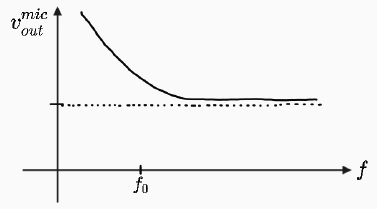
\includegraphics[width=0.46\textwidth]{v_mic_out.png}}
    \hfill
    \subfloat[Normal diaphragm force \(|\tilde{f}_{D\perp}|\) versus distance, showing the transition between \(1/r^2\) near-field and \(1/r\) far-field scaling]{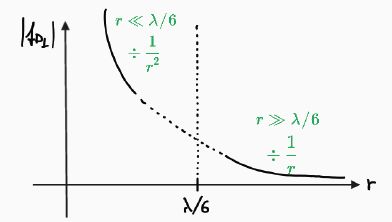
\includegraphics[width=0.46\textwidth]{f_D_perp.png}}
    \caption{Distance and frequency dependence of the pressure-gradient microphone response, illustrating the physical origin of the proximity effect}
\end{figure}

\section{Combination Microphones}

Adding the output of a pressure element to that of a pressure-gradient element produces a directional pattern intermediate between the omnidirectional and the bidirectional extremes.
Denoting the individual outputs as \(v_P(\theta) = v_{P0}\) and \(v_G(\theta) = v_{G0}\cos\theta\), the total microphone voltage is
\[
v_M(\theta) = v_{P0} + v_{G0}\cos\theta = v_{P0}\left(1 + B\cos\theta\right), \qquad B = \frac{v_{G0}}{v_{P0}}
\]
The on-axis value \(v_M(0) = v_{P0}(1+B)\) is the maximum output, so the response normalized to its on-axis maximum defines the directivity function
\[
D(\theta) = \frac{v_M(\theta)}{v_M(0)} = \frac{1+B\cos\theta}{1+B}, \qquad -1 \leq D(\theta) \leq 1
\]
The polar pattern in decibels is obtained as \(20\log_{10}|D(\theta)|\).

\begin{figure}[!htb]
    \centering
    \subfloat[Schematic superposition of pressure and gradient outputs]{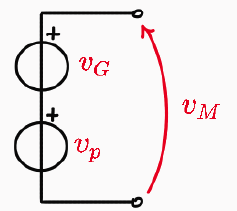
\includegraphics[height=0.2\textheight]{mic_combination.png}}
    \hspace{1cm}
    \subfloat[Cardioid polar pattern (\(B = 1\)): null at \(\theta = 180^\circ\), maximum at \(\theta = 0^\circ\)]{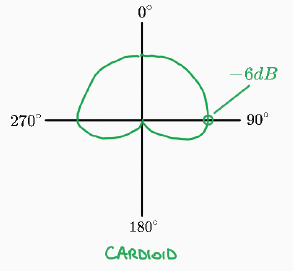
\includegraphics[height=0.2\textheight]{cardioid_pattern.png}}
    \caption{Combination microphone: superposition of pressure and gradient components, with the cardioid (\(B = 1\)) as the most common special case}
\end{figure}

The three canonical limiting patterns correspond to \(B = 0\) (only the pressure component survives, \(D = 1\), omnidirectional), \(B = 1\) (cardioid, \(v_M = v_{P0}(1 + \cos\theta)\), zero at \(\theta = 180^\circ\)), and \(B \to \infty\) (only the gradient survives, \(D \to \cos\theta\), bidirectional figure-eight).
The cardioid case at \(B = 1\) is worth noting in detail: the output at \(\theta = 0^\circ\) equals \(2v_{P0}\), at \(\theta = 90^\circ\) it equals \(v_{P0}\), and at \(\theta = 180^\circ\) it is exactly zero.

\begin{figure}[!htb]
    \centering
    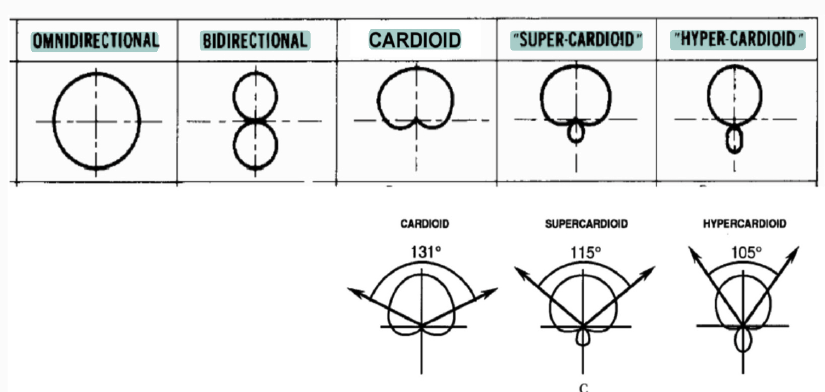
\includegraphics[width=0.65\textwidth]{directivity_pattern.png}
    \caption{A family of polar patterns generated by the combination formula for representative values of \(B\): omnidirectional, cardioid, supercardioid, hypercardioid, and bidirectional}
\end{figure}

\section{Directivity Factor and Polar Patterns}

\subsection{Definition of the Directivity Factor}

A quantitative comparison of directional microphones requires a single figure of merit that captures how much a pattern favors the on-axis direction over a diffuse field.
The directivity factor \(Q\) is defined in a homogeneous, isotropic sound field, where the RMS pressure \(p_{\mathrm{rms}}\) is the same from every direction.
The infinitesimal mean acoustic power arriving from a solid-angle element \(dA = r^2\sin\theta d\theta d\phi\) is
\[
d\overline{W}_A = \frac{p_{\mathrm{rms}}^2}{\rho_0 c} r^2\sin\theta d\theta d\phi
\]
since the ratio \(\mathrm{Re}[Z_S]/|Z_S|^2 = 1/(\rho_0 c)\) for a spherical wave in the far field.

\begin{figure}[!htb]
    \centering
    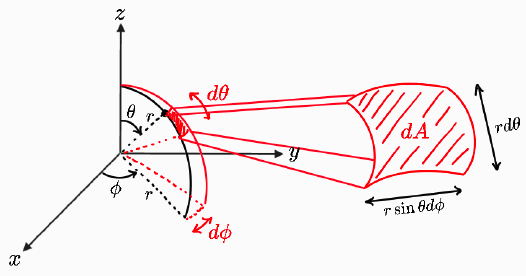
\includegraphics[width=0.50\textwidth]{polar_coord.png}
    \caption{Spherical coordinate geometry for the integration of acoustic power over all incident directions}
\end{figure}

A microphone with directivity function \(D(\theta)\) weights the received power by \(D^2(\theta)\):
\[
d\overline{W}_{A,M} = \frac{p_{\mathrm{rms}}^2}{\rho_0 c} D^2(\theta) r^2\sin\theta d\theta d\phi
\]
Integrating over the full sphere and exploiting azimuthal symmetry:
\[
\overline{W}_{A,M} = \frac{2\pi r^2 p_{\mathrm{rms}}^2}{\rho_0 c}\int_0^{\pi} D^2(\theta)\sin\theta d\theta
\]
For the omnidirectional reference, \(D = 1\) and \(\int_0^\pi\sin\theta d\theta = 2\), so \(\overline{W}_{A,\mathrm{omni}} = 4\pi r^2 p_{\mathrm{rms}}^2/(\rho_0 c)\).
The directivity factor is accordingly defined as
\[
Q = \frac{\overline{W}_{A,\mathrm{omni}}}{\overline{W}_{A,M}} = \frac{2}{\displaystyle\int_0^{\pi} D^2(\theta)\sin\theta d\theta} \geq 1
\]
A directional microphone, by excluding power arriving from unfavorable directions, receives less total power than an omnidirectional one in the same diffuse field, hence \(Q \geq 1\).

\subsection{Directivity Factor for the General Pattern}

Substituting \(D(\theta) = (1+B\cos\theta)/(1+B)\) and evaluating the key integral:
\[
\int_0^{\pi}(1+B\cos\theta)^2\sin\theta d\theta = \frac{6+2B^2}{3}
\]
the directivity factor takes the closed form
\begin{equation}
Q(B) = \frac{3(1+B)^2}{3+B^2}.
\label{eq:directivityFactor}
\end{equation}
The derivative with respect to \(B\) is
\[
\frac{\partial Q}{\partial B} = \frac{6(1+B)(3-B)}{(3+B^2)^2}
\]
which vanishes at \(B = 3\), confirming a maximum at that point with value \(Q_{\mathrm{max}} = Q(3) = 4\), realized by the hypercardioid pattern.

\begin{figure}[!htb]
    \centering
    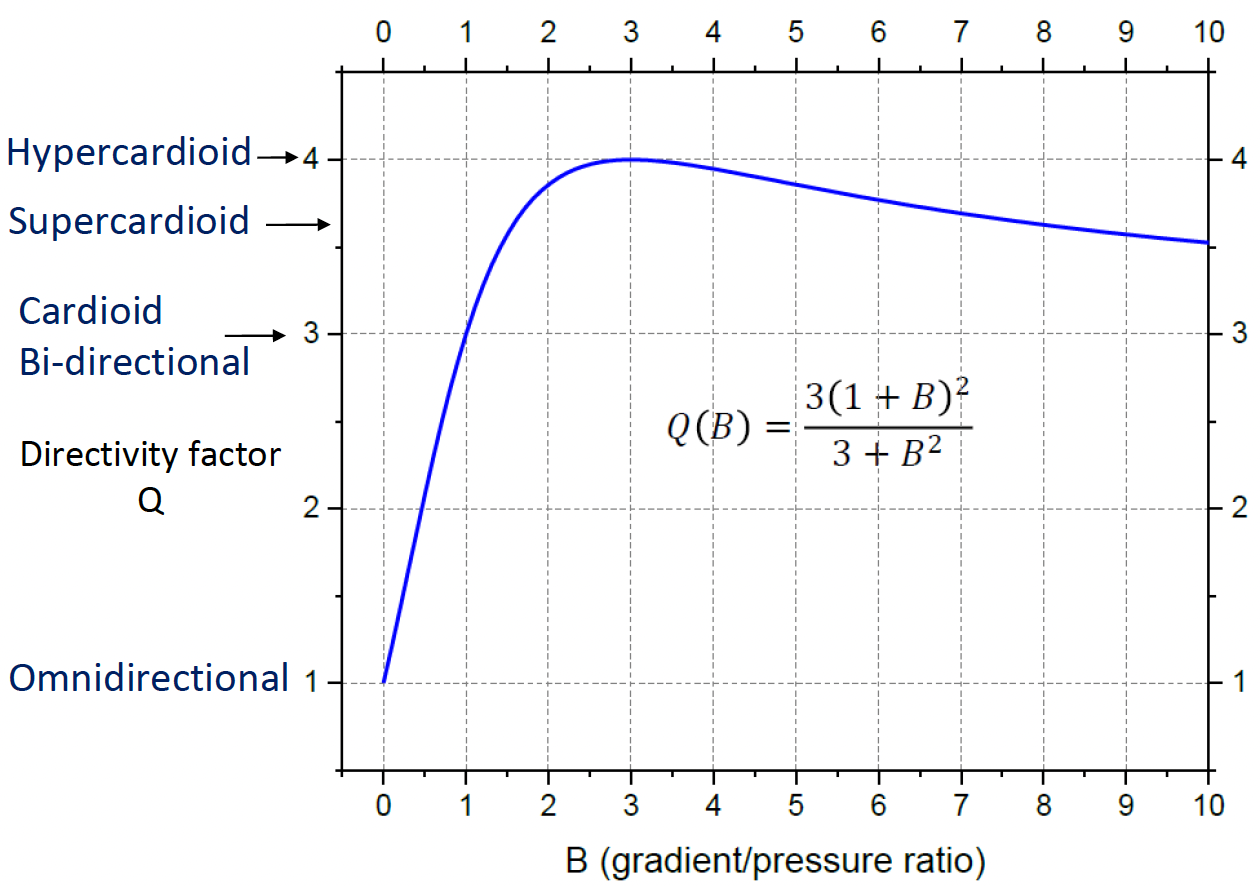
\includegraphics[width=0.55\textwidth]{Q_Factor_Mic.png}
    \caption{Directivity factor \(Q\) as a function of the mixing ratio \(B\), reaching its maximum \(Q = 4\) at \(B = 3\) (hypercardioid)}
\end{figure}

\subsection{Front-to-Rear Ratio}

The front-to-rear ratio \(FR\) quantifies how effectively the microphone rejects sound arriving from the rear hemisphere:
\[
FR = \frac{\overline{W}_{A,\mathrm{front}}}{\overline{W}_{A,\mathrm{rear}}} = \frac{\displaystyle\int_0^{\pi/2} D^2(\theta)\sin\theta d\theta}{\displaystyle\int_{\pi/2}^{\pi} D^2(\theta)\sin\theta d\theta}
\]
Evaluating with the general directivity function gives
\[
FR(B) = \frac{3+3B+B^2}{3-3B+B^2}
\]
Differentiating:
\[
\frac{\partial FR}{\partial B} = \frac{6(3-B^2)}{(3-3B+B^2)^2}
\]
which is zero at \(B = \sqrt{3}\): the front-to-rear ratio is maximized by the supercardioid pattern (\(B = \sqrt{3} \approx 1.7\)).
Note that the hypercardioid (\(B = 3\)) and the supercardioid (\(B = \sqrt{3}\)) optimize two different objectives, and no single value of \(B\) simultaneously maximizes both \(Q\) and \(FR\).

\begin{figure}[!htb]
    \centering
    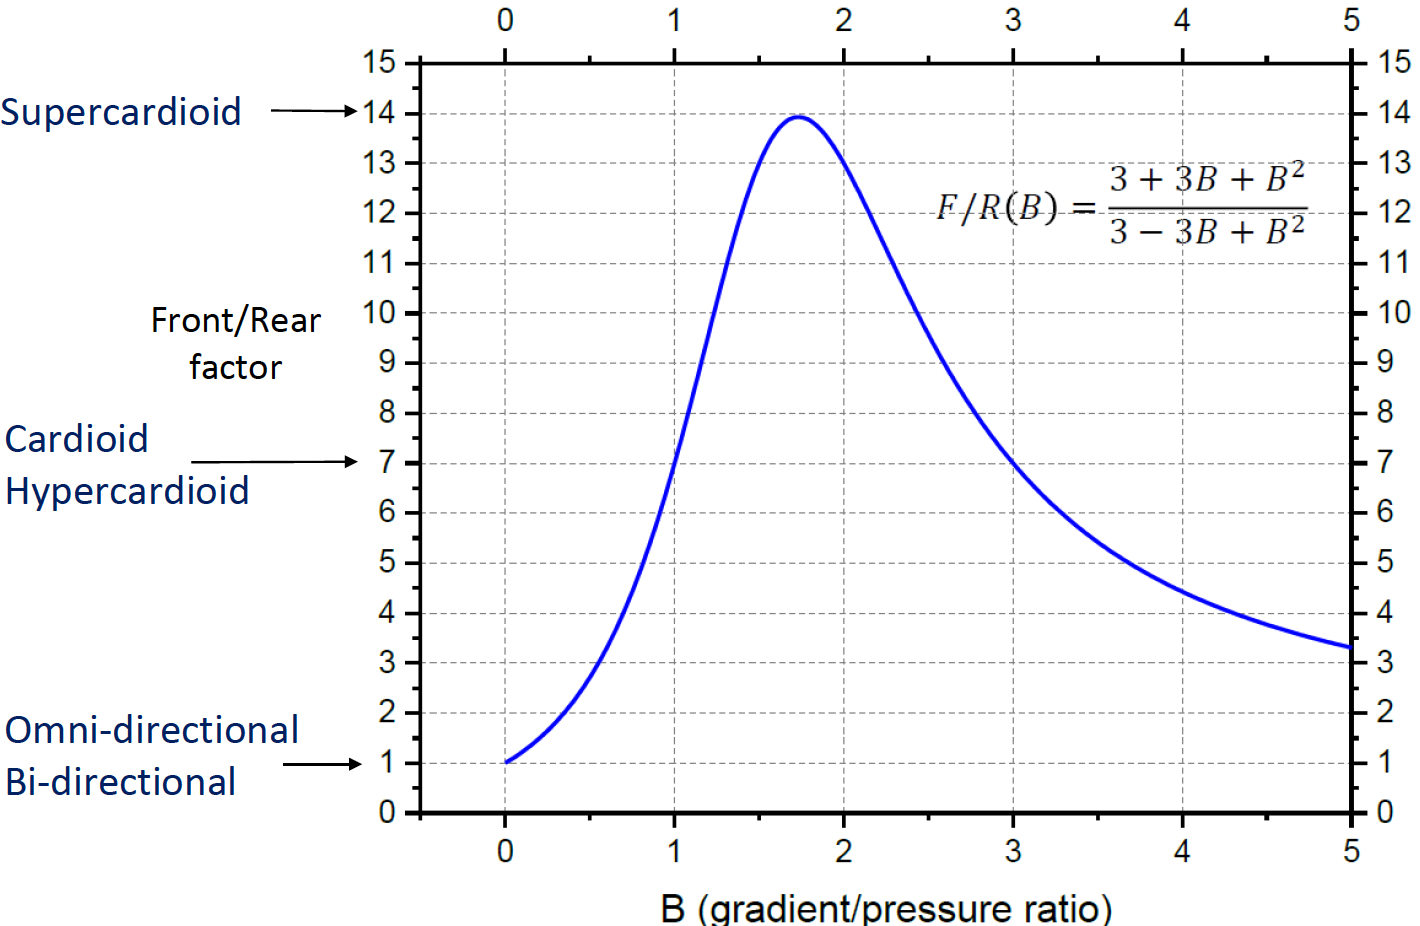
\includegraphics[width=0.55\textwidth]{Front_Rear_Ratio.png}
    \caption{Front-to-rear ratio \(FR\) as a function of \(B\), reaching its maximum at \(B = \sqrt{3}\) for the supercardioid}
\end{figure}

\subsection{Summary of Polar Patterns}

The five standard polar patterns, their mixing ratios, directivity factors from equation \eqref{eq:directivityFactor}, and front-to-rear ratios are collected in table \ref{tab:polarPatterns}.

\begin{table}[!htb]
\centering
\renewcommand{\arraystretch}{1.3}
\begin{tabular}{cccc}
\hline
\textbf{Pattern} & \textbf{\(B = v_{G0}/v_{P0}\)} & \textbf{Directivity factor \(Q\)} & \textbf{Front-to-rear \(FR\)} \\
\hline
Omnidirectional & \(0\)         & \(1\)        & \(1\)  \\
Bidirectional   & \(\infty\)    & \(3\)        & \(1\)  \\
Cardioid        & \(1\)         & \(3\)        & \(7\)  \\
Hypercardioid   & \(3\)         & \(4\)        & \(7\)  \\
Supercardioid   & \(\sqrt{3}\)  & \(\approx 3.7\) & \(14\) \\
\hline
\end{tabular}
\caption{Standard polar patterns and their directivity metrics}
\label{tab:polarPatterns}
\end{table}

Several observations are noteworthy.
The bidirectional and cardioid patterns share \(Q = 3\), despite their different spatial geometry: the bidirectional achieves this through figure-eight nulls at \(\pm 90^\circ\), while the cardioid achieves the same directivity through its smooth rear null at \(180^\circ\).
The hypercardioid at \(B = 3\) achieves the maximum directivity \(Q = 4\), meaning it captures only one quarter of the power received by an omnidirectional microphone in the same diffuse field; however, its front-to-rear ratio of \(7\) is identical to that of the cardioid, because the hypercardioid has a small but non-zero rear lobe.
The supercardioid at \(B = \sqrt{3}\) maximizes the front-to-rear ratio to \(14\), providing the strongest rear rejection at the cost of slightly reduced \(Q\); it is the preferred pattern when ambient noise arrives predominantly from behind the performer.

\section{Physical Realization: Rear-Cavity Model}

The combination formula \(v_M = v_{M0}(1 + B\cos\theta)\) is not merely an abstract superposition of two idealized transducers but can be realized acoustically within a single capsule by introducing a controlled path to the rear of the diaphragm.

\subsection{Structure and Circuit Model}

In the combined microphone, the rear face of the diaphragm communicates with the outside through a back cavity containing an acoustic compliance \(C_A\) (the enclosed air volume) and an acoustic resistance \(R_A\) (a resistive screen or narrow slot).
The front face is exposed directly to the incident field at position \(x_1\), while the rear opening samples the field at a displaced position.

\begin{figure}[!htb]
    \centering
    \subfloat[Physical model of the rear cavity]{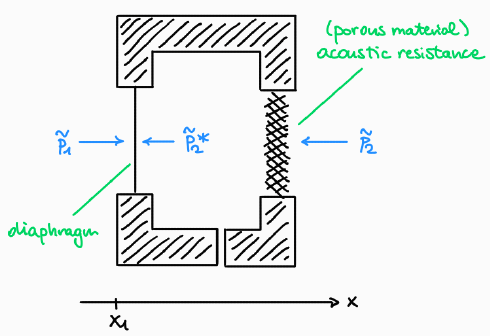
\includegraphics[height=0.21\textheight]{pressure_plus_gradient_mic_model.png}}
    \hfill
    \subfloat[Equivalent acoustic circuit with compliance \(C_A\), resistance \(R_A\), and diaphragm impedance \(Z_{AD}\)]{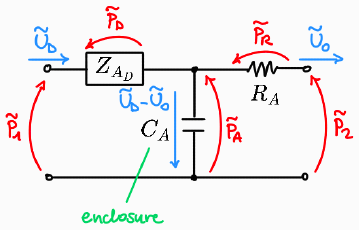
\includegraphics[height=0.21\textheight]{pressure_plus_grad_mic_circuit.png}}
    \caption{Combined pressure and pressure-gradient microphone: rear-cavity structure and its equivalent acoustic circuit}
\end{figure}

For a plane wave \(\tilde{p} = p_0 e^{-jkx}\), the front pressure is \(\tilde{p}_1 = p_0 e^{-jkx_1}\) and the pressure at the rear opening is, to first order in \(\Delta l\),
\[
\tilde{p}_2 = \tilde{p}_1\left(1 - j\frac{\omega}{c} \Delta l \cos\theta\right)
\]
Applying acoustic Kirchhoff laws to the equivalent circuit, with \(\tilde{U}_D\) and \(\tilde{U}_0\) denoting the volume velocities at the diaphragm and the rear port respectively, gives the pair of equations:
\[
\begin{cases}
\tilde{p}_1 = \dfrac{1}{j\omega C_A}(\tilde{U}_D - \tilde{U}_0) + Z_{AD} \tilde{U}_D \\[6pt]
\tilde{p}_2 = \dfrac{1}{j\omega C_A}(\tilde{U}_D - \tilde{U}_0) - R_A \tilde{U}_0
\end{cases}
\]
where \(Z_{AD}\) is the radiation impedance of the diaphragm.

\subsection{Differential Pressure and the Mixing Parameter}

Solving for the differential pressure \(\tilde{p}_D\) acting across the diaphragm:
\[
\tilde{p}_D = \tilde{p}_1\;\frac{Z_{AD} R_A\!\left[1 + \dfrac{\Delta l\cos\theta}{c R_A C_A}\right]}{Z_{AD} R_A - j \dfrac{R_A + Z_{AD}}{\omega C_A}}
\]
Defining the frequency-dependent complex amplitude
\[
A = \frac{Z_{AD} R_A}{Z_{AD} R_A - j \dfrac{R_A + Z_{AD}}{\omega C_A}}
\]
and the dimensionless mixing parameter
\[
B = \frac{\Delta l}{c R_A C_A}
\]
the magnitude of the net diaphragm force is
\[
|\tilde{f}_D| = \tilde{p}_D S_D = \tilde{p}_1 S_D |A| (1 + B\cos\theta)
\]
The output voltage, proportional to this force, recovers the general combination pattern:
\[
\tilde{v}_M = \tilde{v}_{M0} (1 + B\cos\theta)
\]
The mixing ratio \(B\) is governed by the acoustic time constant \(R_A C_A\) of the rear cavity: a shorter time constant (smaller compliance or larger resistance) increases \(B\), shifting the pattern from omnidirectional toward the hypercardioid.
At \(B = 0\), corresponding to a sealed cavity (\(R_A \to \infty\)), only the pressure component survives and the pattern is omnidirectional.
As \(B\) increases through \(1\), \(\sqrt{3}\), and \(3\), the capsule realizes the cardioid, supercardioid, and hypercardioid patterns in turn.
Multiple polar patterns can therefore be selected from a single capsule by varying the acoustic resistance of the rear cavity, a principle exploited in multi-pattern studio microphones.

    
\end{document}
